%%\documentclass[preprint,12pt,authoryear]{elsarticle}

%% Use the option review to obtain double line spacing
%%\documentclass[preprint,12pt]{elsarticle}

%% Use the options 1p,twocolumn; 3p; 3p,twocolumn; 5p; or 5p,twocolumn
%% for a journal layout:
%% \documentclass[final,1p,times]{elsarticle}
%% \documentclass[final,1p,times,twocolumn,longtitle]{elsarticle}
 \documentclass[final,3p,times]{elsarticle}
%% \documentclass[final,3p,times,twocolumn,longtitle]{elsarticle}
%% \documentclass[final,5p,times]{elsarticle}
%% \documentclass[final,5p,times,longtitle,twocolumn]{elsarticle}

%% For including figures, graphicx.sty has been loaded in
%% elsarticle.cls. If you prefer to use the old commands
%% please give \usepackage{epsfig}

%% The amssymb package provides various useful mathematical symbols
\usepackage{amssymb}
\usepackage{amsmath}
%% The amsthm package provides extended theorem environments
\usepackage{amsthm}

\usepackage{lipsum}
\usepackage{graphicx}% Include figure files
\usepackage{dcolumn}% Align table columns on decimal point
\usepackage{bm}% bold math
\usepackage{multirow}% multirow for tables
\usepackage{comment}% commenting blocks
%\usepackage{subfig}
\usepackage{subfigure}
\usepackage{soul}

%\usepackage[square]{natbib}
\usepackage[usenames,dvipsnames]{color}
\usepackage{hyperref}% add hypertext capabilities

% The line numbering messes up the title. Comment out these lines and
% the title page will be fine.
\usepackage[mathlines]{lineno}% Enable numbering of text and display math

\usepackage{lineno}
\usepackage{setspace}

\usepackage{verbatim} % Added by AE for multiline comments

\DeclareGraphicsExtensions{.pdf,.png,.jpg}

\bibliographystyle{model1-num-names}
\biboptions{sort&compress}

%\usepackage[font=small,skip=0pt]{caption}
%\usepackage[showframe,%Uncomment any one of the following lines to test 
%scale=0.7, marginratio={1:1, 2:3}, ignoreall,% default settings
%%text={7in,10in},centering,
%%margin=1.5in,
%%total={6.5in,8.75in}, top=1.2in, left=0.9in, includefoot,
%%height=10in,a5paper,hmargin={3cm,0.8in},
%]{geometry}
%

\journal{Nuclear~Instruments~and~Methods~A}


\begin{document}


\newcommand\JOcom[1]{{\textcolor{red}{#1}}}

\newcommand{\bmd}{$\beta$}
\newcommand{\bpd}{$\beta^{+}$}
\newcommand{\bb}{$\beta\beta$}
\newcommand{\nbb}{\ensuremath{\nu\beta\beta}}
%\newcommand
\newcommand{\Te}{$^{130}$Te}
\newcommand{\Se}{$^{82}$Se}
\newcommand{\B}{$^{8}$B}
\newcommand{\Bten}{$^{10}$B}
\newcommand{\Cten}{$^{10}$C}
\newcommand{\C}{$^{10}$C}


\graphicspath{{plots/}}

\title{Separating double-beta decay events from solar neutrino
  interactions in kiloton-scale liquid scintillator detectors}
\author[UChicago]{Andrey Elagin\corref{cor1}}
\cortext[cor1]{Corresponding Author: \href{mailto:elagin@hep.uchicago.edu}{\tt{elagin@hep.uchicago.edu}}}
\author[UChicago]{Henry J. Frisch}
\author[MIT,LBL]{Jonathan Ouellet}
\author[MIT]{Lindley Winslow}
\author[OPTIN]{{\bf Opt in}}


\address[UChicago]{ Enrico Fermi Institute, University of Chicago, Chicago, IL, 60637 }
\address[MIT]{ Massachusetts Institute of Technology, Cambridge, MA 02139 }
\address[LBL]{ Nuclear Science Division, Lawrence Berkeley National Labo\
ratory, Berkeley, CA 94720 }
\address[OPTIN]{{\bf Please opt-in if you think you should be on the author list}}


\begin{abstract}
We present a technique for separating double beta decay (\bb-decay) events from 
background due to \B~solar neutrino interactions. This background becomes dominant 
in a kilo-ton scale liquid scintillator detector. In searches for the neutrinoless 
double beta decay (0\nbb-decay) \B~background is usually considered as irreducible 
due to an overlap in the energy deposition. We note that in a liquid scintillator 
detector electrons from 0\nbb-decay often exceed Cherenkov threshold. Selection of 
early photons using fast photo-detectors separates prompt directional Cherenkov 
light from delayed isotropic scintillation light. This leads to the possibility of 
reconstructing the event topology of 0\nbb-decay candidate events by analyzing 
spatial distribution of early photons. Using a simulation of a 6.5~m radius liquid 
scintillator detector with 100~ps resolution photo-detectors, we perform a 
spherical harmonics analysis of the early light emitted in each candidate event and 
show the difference between 0\nbb-decay signal and \B~background events. We discuss 
key detector parameters that affect the separation power.


%We propose a technique for separating 0{\nbb}-decay events from
%background due to $^{10}$C decays and $^8$B solar neutrino
%interactions in a liquid scintillator detector. These represent the
%key backgrounds at shallow and deep sites. In particular, we focus
%on \B~background suppression which is traditionally viewed as irreducible
%background to 0\nbb-decay searches. The technique compares
%event topology of the signal and background events using spherical
%harmonics analysis of the early light emitted in signal and
%background events. Selection of early photons using fast photo-detectors
%allows for separation of directional Cherenkov from isotropic
%scintillation light and identification of event topologies based
%on the spatial distribution of the early photons in the detector.

\end{abstract}

\date{\today}

\maketitle

\tableofcontents

\linenumbers\relax % Commence numbering lines

\section{Introduction}

Over the past decade, neutrino oscillation experiments have
conclusively established that neutrinos have mass. However, one of the
most fundamental and still open questions in particle physics is the
nature of that mass. Is the neutrino unique in the Standard Model with
a Majorana type mass, as is predicted by most theoretical arguments,
or does it have a Dirac type mass, like the rest of the fermions in
the Standard Model? A Majorana mass would have far reaching
implications, from explaining the lightness of the neutrino and
providing a bridge to higher energy phenomena through the see-saw
mechanism [CITATION] to providing the required lepton-number violation
(LNV) and {\sf CP}-violation needed for leptogenesis to explain the
baryon asymmetry of the universe \cite{Luty1992}. Conversely, a Dirac
neutrino could point to an underlying symmetry of the Universe.
Presently, the most promising technique for answering these questions
is the search for Neutrinoless Double-Beta (0\nbb) decay
[CITATION]. In this decay, a nucleus undergoes a second order
$\beta$-decay without producing any neutrinos,
$(Z,A)\rightarrow(Z+2,A)+2\beta^-$. The resulting decay products are
ejected with a total kinetic energy equal to the decay $Q$-value, and
most of this is carried by the electrons which have typical kinetic
energies of $\sim$1--2~MeV.

The standard mechanism of 0{\nbb} decay is parameterized by the
\emph{effective Majorana mass},
\mbox{$m_{\beta\beta}\equiv\left|\sum_i U^2_{ei}m_i\right|$}, where
$U_{ei}$ are the elements of the PMNS matrix and $m_i$ are the
neutrino masses [CITATION].  Recently, this search has generated a
significant amount of experimental interest, with current experiments
searching for 0\nbb decay of $^{76}$Ge \cite{GERDA2013}, $^{130}$Te
\cite{CUORE2015} and $^{136}$Xe \cite{EXO2014,KamLANDZen2013}. At
present, 0{\nbb} decay has never been convincingly observed, but
limits place the half-lives at longer than $10^{23}$--$10^{25}$~yr in
the isotopes studied. These limits translate to a limit on
\mbox{$m_{\beta\beta}\lesssim 150$--$700$~meV}, with the majority of
the spread on this limit coming from uncertainty in the nuclear
modeling. The next generation of 0{\nbb} decay experiments seek to be
sensitive enough to detect or rule out 0{\nbb} decay down to
\mbox{$m_{\beta\beta}<10$~meV}. This will require, among other things,
$\sim$a ton of active isotope, a good energy resolution, and a near
zero background in the region of interest (ROI) [CITATION?].

Over the past few years, liquid scintillator-based detectors have
proven to be a competitive technology in this search
[CITATION?]. Their primary advantage is in their scalability to larger
active masses, which entails disolving larger amounts of active
isotope into the liquid scintillator (LS). This feature allows for
rapid scaling to the 1~ton or more of active isotope. In a large LS
detector, where backgrounds from the outside of the detector can be
efficiently self-shielded or tagged and vetoed, the two backgrounds
relavent to 0{\nbb} decay are 2{\nbb} and electron scattering (ES) interactions of $^{8}$B solar neutrinos.

Two neutrino double beta (2{\nbb}) decay is the Standard Model allowed
second order $\beta$-decay channel where lepton number is conserved,
\mbox{$(Z,A)\rightarrow(Z,A+2)+2\beta+2\bar\nu_e$}. Since the kinetic
energy of the neutrinos is practically never detected, the resulting
2{\nbb} spectrum is broadened from 0~MeV up to the decay
$Q$-value. The high energy tail of this spectrum forms a background
for the 0{\nbb} signal. Since it is intrinsic to the target isotope
and the decay kinematics are nearly identical to 0{\nbb} decay,
2{\nbb} can only be separated from 0{\nbb} with a detector with
powerful enough resolution (see Fig.~\ref{fig:SNOp_bkgs}). Present
LS-based detectors achieve typical energy resolutions of
\mbox{$\sigma(E)\sim 5\%/\sqrt{E(\rm MeV)}$}. The next generation of
detectors will improve up this... \JOcom{Something about
  photo-coverage (etc). Eventually this will fold back in the question
  of slowing down the scintillation signal and improving the Cherenkov
  signal at the cost of decreasing the total light yield.}
  
  
The spectrum of ES interactions of $^{8}$B solar neutrinos falls
slowly over the range 2--3~MeV, creating a nearly flat background
across the 0{\nbb} ROI. However, these interactions produce only a
single $\sim$2.5~MeV electron, rather than two $\sim$1.2~MeV electrons
as in 0{\nbb}. In a LS, this difference in event topology manifests as
two distinct distributions of Cherenkov photons, and thus creates a
way to tag and remove these $^{8}$B solar neutrino events. As we have
shown in previous works, photo-detectors with timing resolution of
$\sim$100~ps can resolve the prompt Cherenkov photons from the slower
scintillation signal \cite{Aberle2014}. The challenge is that for a
given event, we expect XXX Cherenkov photons with which to reconstruct
the event topology.

In this paper, we proposed to use a spherical harmonic decomposition
to analyze the distribution of early photo-electrons (PE) to
discriminate between $^{8}$B solar neutrinos and 0{\nbb} decay
events. In Section~\ref{sec:detector_description}, we describe the
detector model we will use throughout this paper. In
Section~\ref{sec:spherical_harmonics}, we introduce the spherical
harmonic decomposition, and discuss the performance of this analysis
in Section~\ref{sec:performance_and_challenges}.






\begin{figure}[ht]
  \centering
  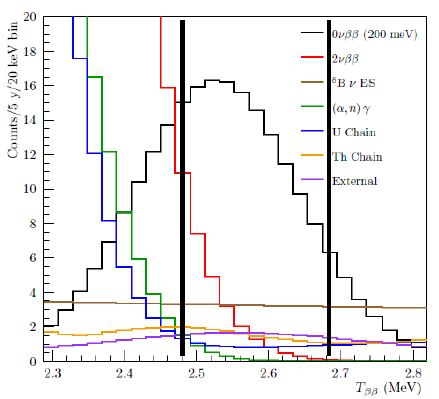
\includegraphics[width=0.75\columnwidth]{SNOp_backgrounds.JPG}
  \caption{SNO+ Phase I signal and background energy spectrum (visible
    kinetic energy reconstructed under a 0{\nbb} hypothesis). Plot
    taken from~\cite{SNOp_paper}}
  \label{fig:SNOp_bkgs}
\end{figure}

\begin{figure*}[ht]
  \centering
  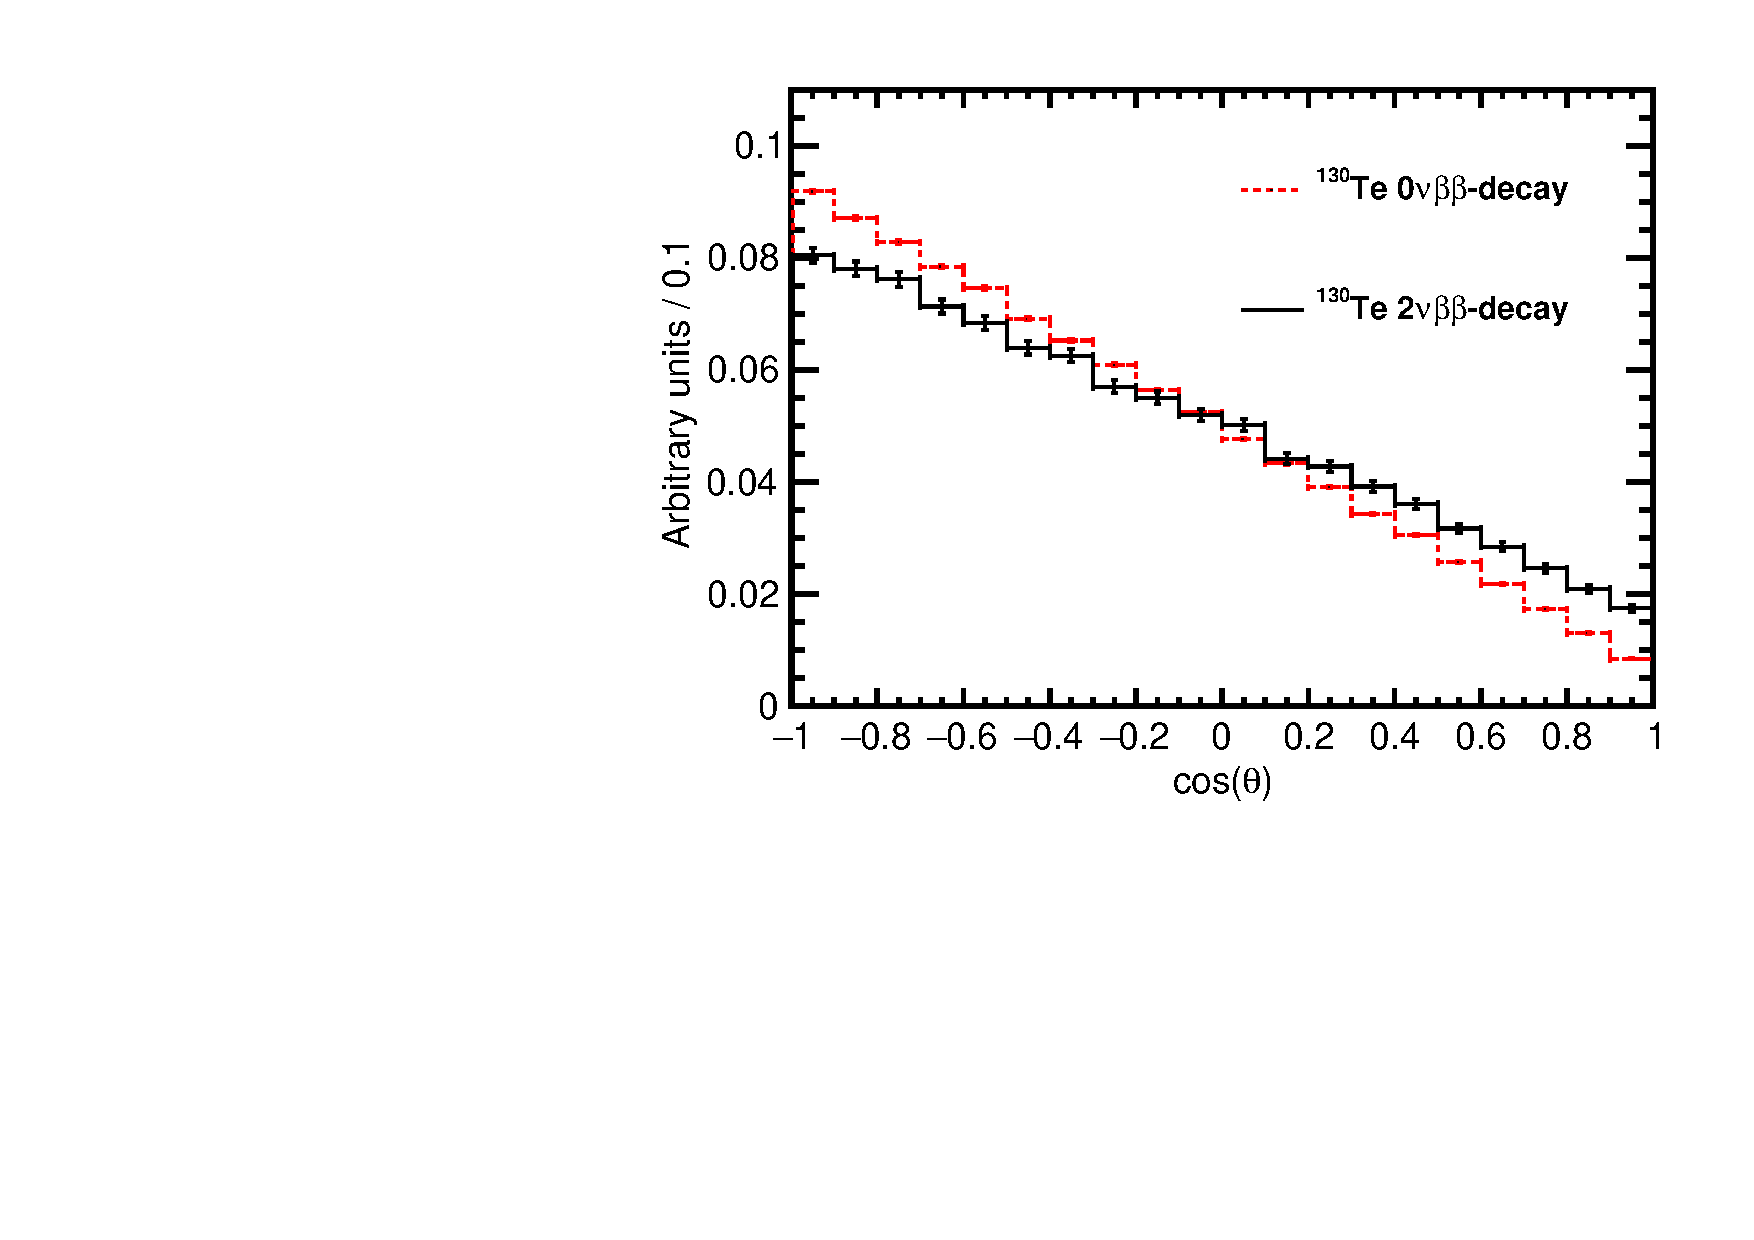
\includegraphics[width=0.49\textwidth]{hCos_Te130.pdf}
  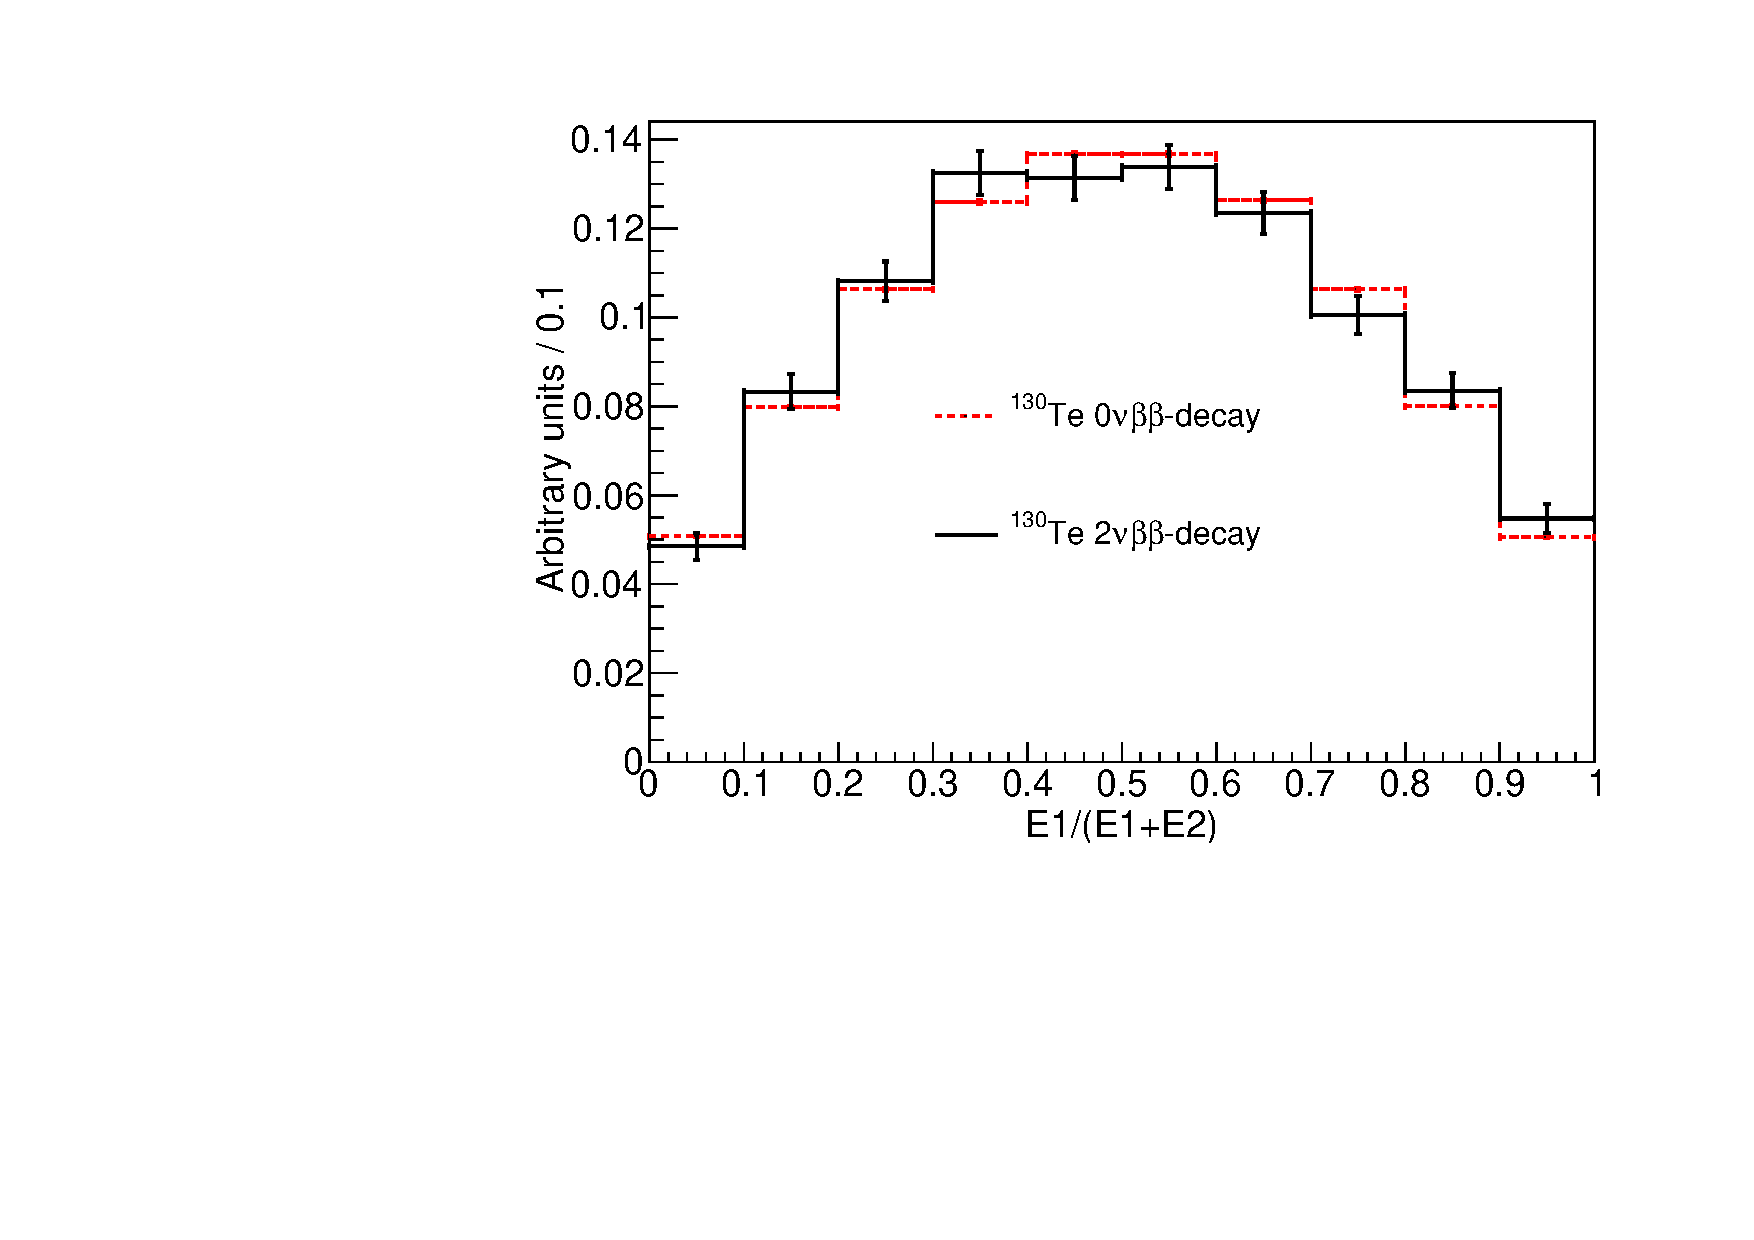
\includegraphics[width=0.49\textwidth]{hE1toQ_Te130.pdf}
  \caption{Comparison between kinematics of 0{\nbb} (\emph{dashed red
      lines}) and 2{\nbb} decays (\emph{solid black lines}) for events
    with the total kinetic energy of the electrons above 90\% of the
    Q-value. \emph{Left:} Cosine of the angle between two
    electrons. \emph{Right:} Fraction of energy carried by one of the
    two electrons. Due to limited statistic around the energy spectrum
    end point for 2{\nbb} decay we show statistical errors for each
    bin.}
  \label{fig:Kinematics}
\end{figure*}

\section{Detector Model}
\label{sec:detector_description}

In order to study the topology of $\vbb$ decay and background events in a liquid scintillator detector, a Geant4\cite{geant4one,geant4two} simulation has been constructed. This is the same simulation used in our preceding paper~\cite{Aberle2014}. Therefore, we limit out discussion of the simulation to a summary of the the most relevant simulation parameters.

The simulation uses Geant4~version 4.9.6.  We use the default liquid scintillator optical model, in which optical photons are assigned the group velocity in the wavelength region of normal dispersion.

The detector geometry is a sphere of 6.5~m radius filled with
scintillator. The default scintillator composition has been chosen to match a KamLAND-like
scintillator\cite{kamland2003}: 80\% n-dodecane, 20\% pseudocumene and 1.52~g/l PPO. The
scintillator properties implemented in the simulation include 
\begin{itemize}
\item the atomic composition and density ($\rho$ = 0.78~g/ml), 
\item the wavelength-dependent attenuation length\cite{tajimaMaster} and refractive index\cite{OlegThesis}, 
\item the scintillation emission spectrum\cite{tajimaMaster}, 
\item emission rise time ($\tau_r$ = 1.0~ns) and emission decay time constants ($\tau_{d1}$ = 6.9~ns and $\tau_{d2}$ = 8.8~ns with relative weights of 0.87 and 0.13)\cite{tajimaThesis}, 
\item scintillator light yield (9030 photons/MeV), and 
\item the Birks constant ($kB$ $\approx$ 0.1~mm/MeV)\cite{ChrisThesis}.  
\end{itemize}
The attenuation length at 400~nm, which is the position of the peak standard bialkali photocathode efficiency, is 25~m. The attenuation length drops precipitously from 6.5~m to 0.65~m between 370~nm and 360~nm. We use this drop to define the cutoff wavelength at 370~nm. This is a standard scintillator. However, we do deviate from the baseline KamLAND case in that the re-emission of absorbed photons in the scintillator bulk volume and optical scattering, specifically Rayleigh scattering, has not yet been included. A test simulation shows that the effect of optical scattering is negligible~\cite{Aberle2014}.

The inner sphere surface is used as the photodetector. It is treated
as fully absorbing (no reflections), with a photodetector coverage of
100\%. As in the case of optical scattering, reflections at the sphere are a small effect that would create a small tail at longer times. The default is the QE of a bialkali photocathode (Hamamatsu
R7081 PMT)\cite{Hamamatsu_R7081}. The QE values as a function of wavelength come from the Double Chooz\cite{dctwo}
Monte Carlo simulation. We note that the KamLAND 17-inch PMTs use the
same photocathode type with similar quantum efficiency. We are neglecting any threshold effects in the photodetector readout electronics.


Four effects primarily contribute to the timing of the scintillator detector
system: the travel time of the particle, the time constants of the scintillation process, chromatic dispersion, and the timing of the photodetector.

In the energy range important for $0\nu\beta\beta$, a 1.4~MeV electron travels a total path length of 0.8~cm, has a distance from the origin of 0.6~cm in 0.030$\pm$0.004~ns  and takes 0.028$\pm$0.004~ns to drop below Cherenkov threshold. We note that due to scattering of the electron, the final direction of the electron before it stops does not correspond to the initial direction; however the scattering angle is small while the majority of Cherenkov light is produced. The Cherenkov light thus still encodes the direction of the primary electron. The scattering physics is handled by Geant4's ``Multiple Scattering" process which is valid down to 1~keV, where atomic shell structure becomes important\cite{geant4scatt}.


The scintillator-specific rise and decay times are the second effect that determines the timing in a scintillator detector. The first step in the scintillation process is the transfer of energy from the solvent to the solute. The time constant of this
energy transfer accounts for a rise time in scintillation light
emission. Because past neutrino experiments were not highly sensitive to the
effect of the scintillation rise time, there is a lack of accurate measurements of this property. We assume a rise time of 1.0~ns -- but more
detailed studies are needed in the future. The two time constants used
to describe the falling edge of the scintillator emission time
distribution (quoted above) are values specific to the KamLAND scintillator.

Chromatic dispersion is the third effect that determines the timing in a scintillator detector. Due to the wavelength-dependence of the refractive index the speed of
light in the scintillator increases
with increasing photon wavelengths for normal dispersion, with red
light traveling faster than blue light.

Photoelectrons coming from Cherenkov light are on average
created about 0.5~ns earlier than PEs from scintillation light. The
RMS values from PE time distributions for Cherenkov and scintillation
light are both about 0.5~ns. Note that these numbers include the
effect of the finite electron travel time.

The fourth effect determining the timing in a scintillator detector is the timing of the photodetectors. The measurement of the arrival times of single photoelectrons is
affected by the transit-time spread (TTS) of the photodetectors, a
number which can be different by orders of magnitude depending on the
detector type. We use a TTS of 0.1~ns ($\sigma$), which can be achieved with large area picosecond photodetectors
(LAPPDs)\cite{anode_paper,PSEC4_paper,RSI_paper,Vienna2013,Ceramic_paper1,HV_paper,Timing_paper,Incom_paper}.

The primary quantities provided by the Geant4~simulation are the photoelectron hit
positions and the detection times after the TTS resolution has been
applied. These quantities are then used for event topology reconstruction.

Figures~\ref{fig:ArrivalTimeDist} and~\ref{fig:NPhotDist} show the output of the detector simulation discussed in this section. Left panel in Fig.~\ref{fig:ArrivalTimeDist} compares PE arrival time between Cherenkov and scintillation light for 1000 simulated $\Te$ $\vbb$-decay events. The right panel in Fig.~\ref{fig:ArrivalTimeDist} compares the Cherenkov PE arrival times between $\Te$ $\vbb$-decay and $\B$ events. $\B$ events produce a slightly higher number of the Cherenkov photons because they have only one electron carrying the same kinetic energy as opposed to the two electrons in the case of $\vbb$-decay events. Distributions of the scintillation PEs' arrival time are indistinguishable between $^{130}$Te 0{\nbb} decay and $^8$B due to identical total energy in the event, $Q(^{130}{\rm Te})=2.526$~MeV.

\begin{figure*}[ht]
  \centering
  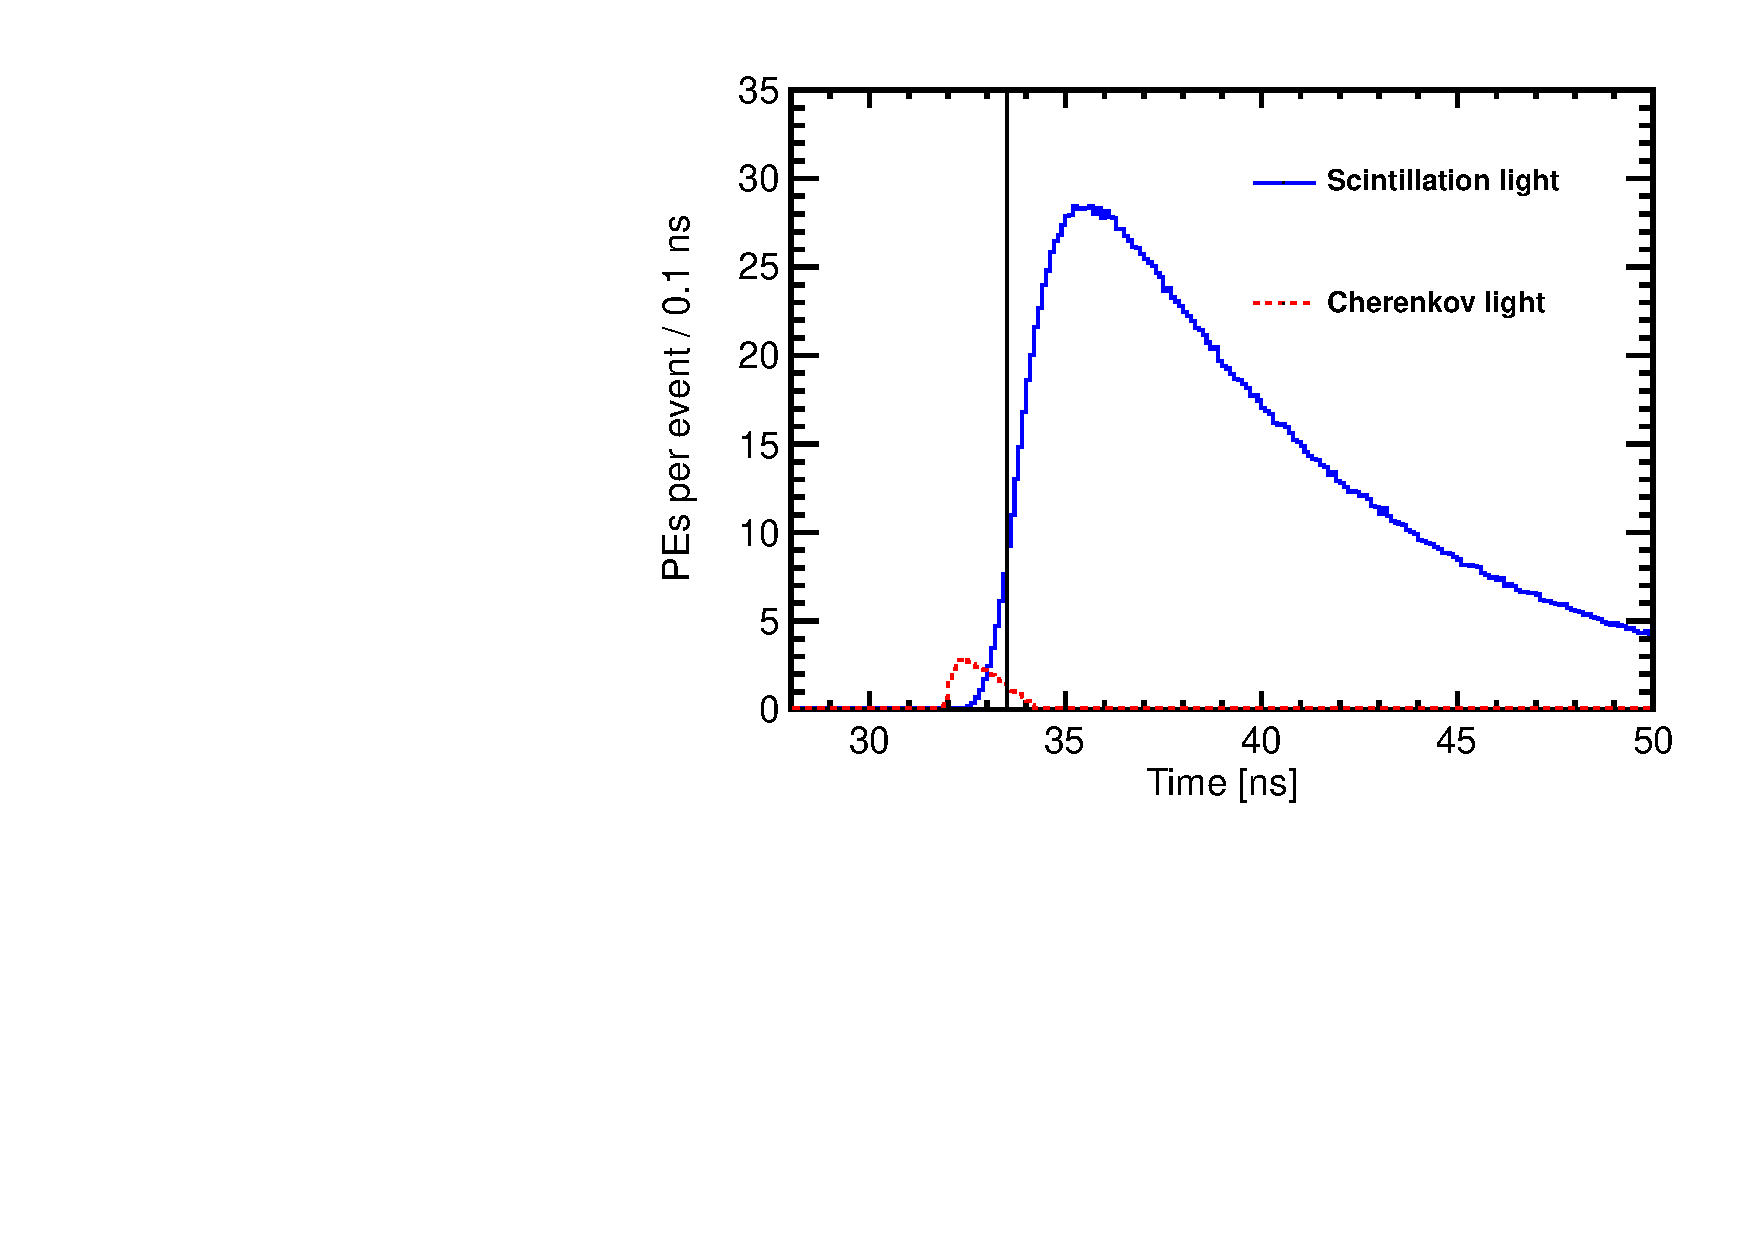
\includegraphics[width=0.45\textwidth]{hT_Te130.pdf}
  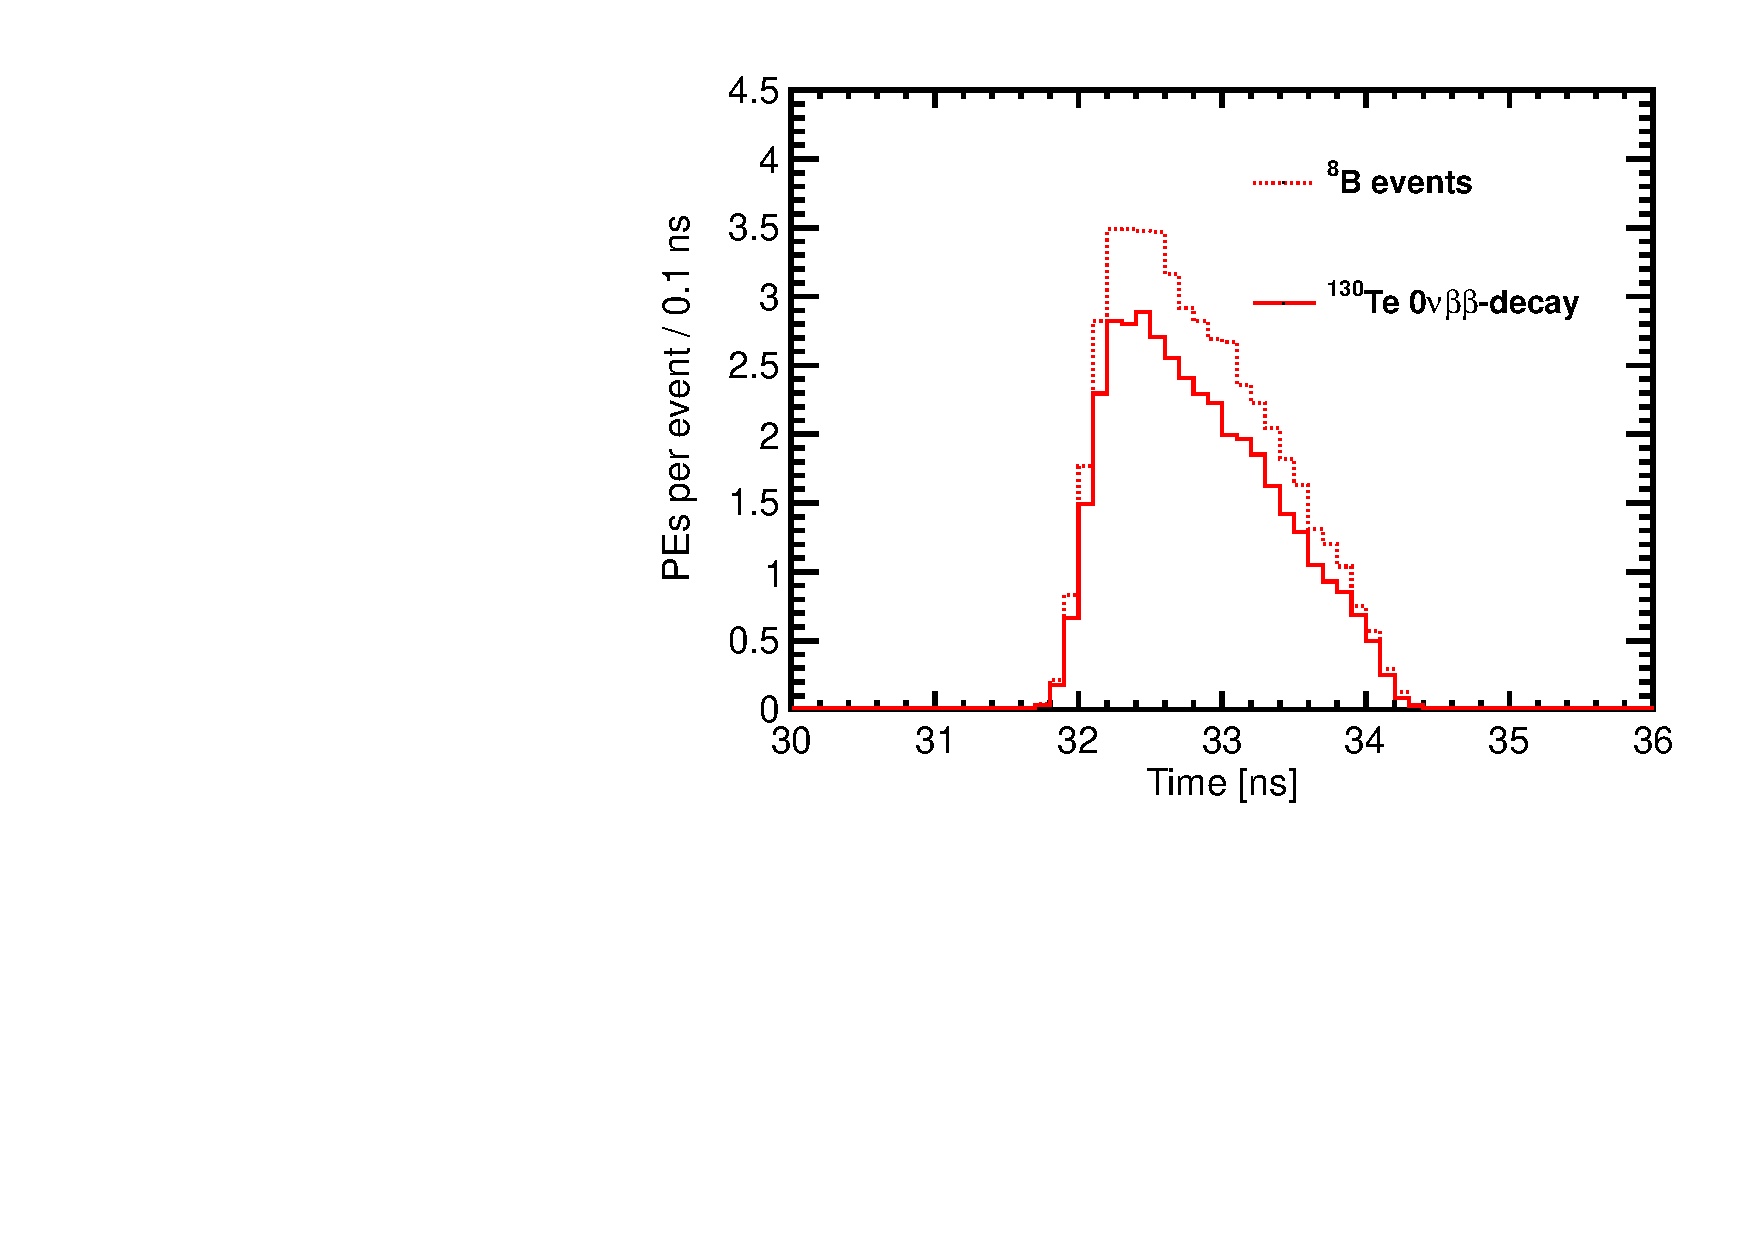
\includegraphics[width=0.45\textwidth]{hTche_Te130_B8.pdf}
  \caption{\emph{Left:} Photo-electron (PE) arrival times after
    application of the photo-detector transit time spread (TTS) of
    100~ps for the simulation of 1000 0{\nbb} decay events of
    $^{130}$Te at the center of the detector. PEs from Cherenkov light
    (\emph{dashed red line}) and scintillation light (\emph{solid blue
      line}) are compared. The black vertical line illustrates a time
    cut at 33.5 ns. \emph{Right:} Comparison between Cherenkov PEs
    arrival time for $^{130}$Te {0\nbb} decay (\emph{solid line}) and
    $^{8}$B (\emph{dotted line}) events. {\bf Distributions of the
      scintillation PEs arrival time are indistinguishable between
      $^{130}$Te 0{\nbb} decay and $^8$B due to identical total energy
      in the event, $Q(^{130}{\rm Te})=2.526$~MeV.} }
\label{fig:ArrivalTimeDist}
\end{figure*}

As shown in Fig.~\ref{fig:ArrivalTimeDist}, a time cut of 33.5~ns on the PE arrival time selects a sample of early PEs that includes the majority of Cherenkov photons. Scintillation PEs also are selected with this time cut. Figure~\ref{fig:NPhotDist} shows the total number of scintillation and Cherenkov PE per event for $\vbb$ signal and $\B$ background events. 
The $\B$ events do have a higher number of Cherenkov PEs on average compared to $\vbb$ events because of the single electron in $\B$ events has a higher energy than the two electrons from $\vbb$ decay.   This difference, though, is not significant enough to be used alone as a reliable discriminant between $\vbb$-decay and $\B$ events.  However, it may provide an extra handle on signal-background separation in combination (e.g. by using multivariative techniques) with other event parameters.

\begin{figure*}[ht]
  \centering
  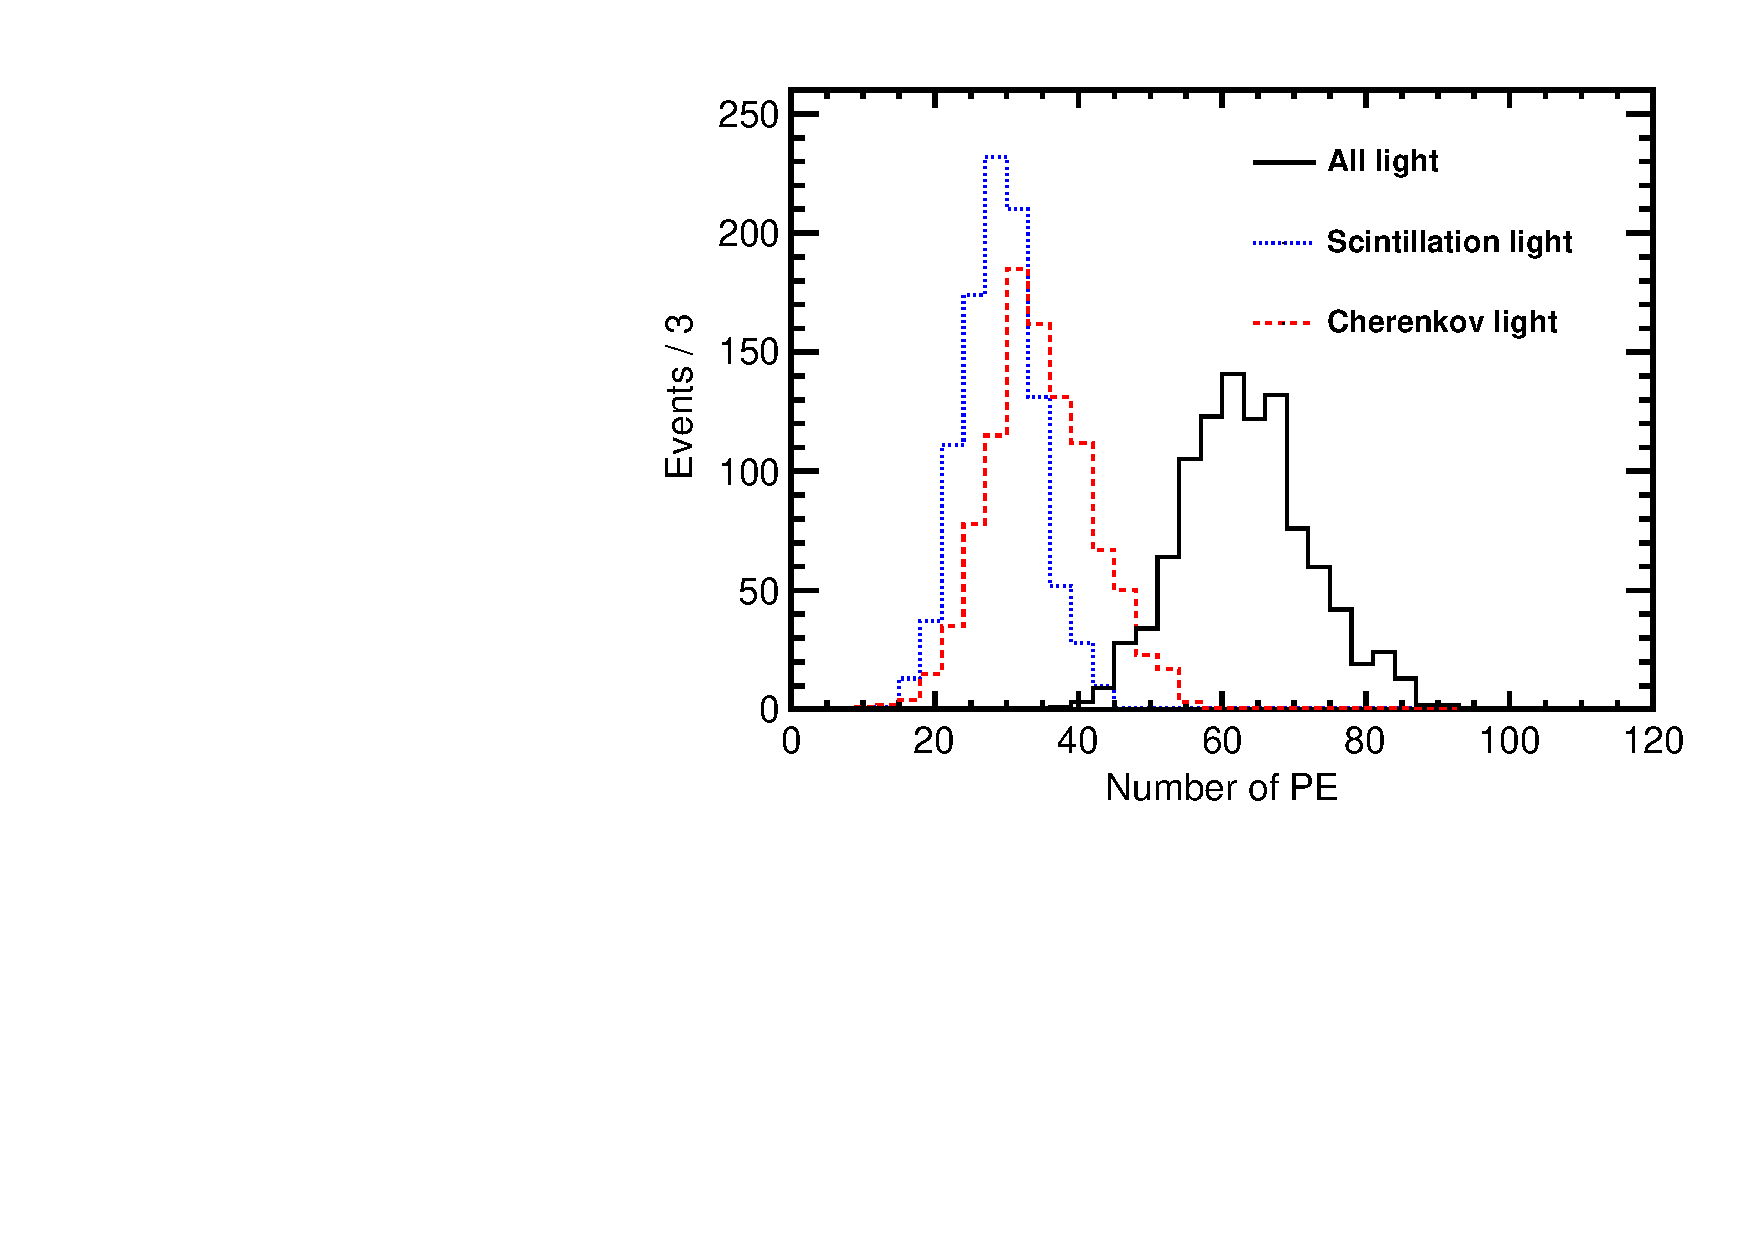
\includegraphics[width=0.45\textwidth]{hMomNPhot_Te130.pdf}
  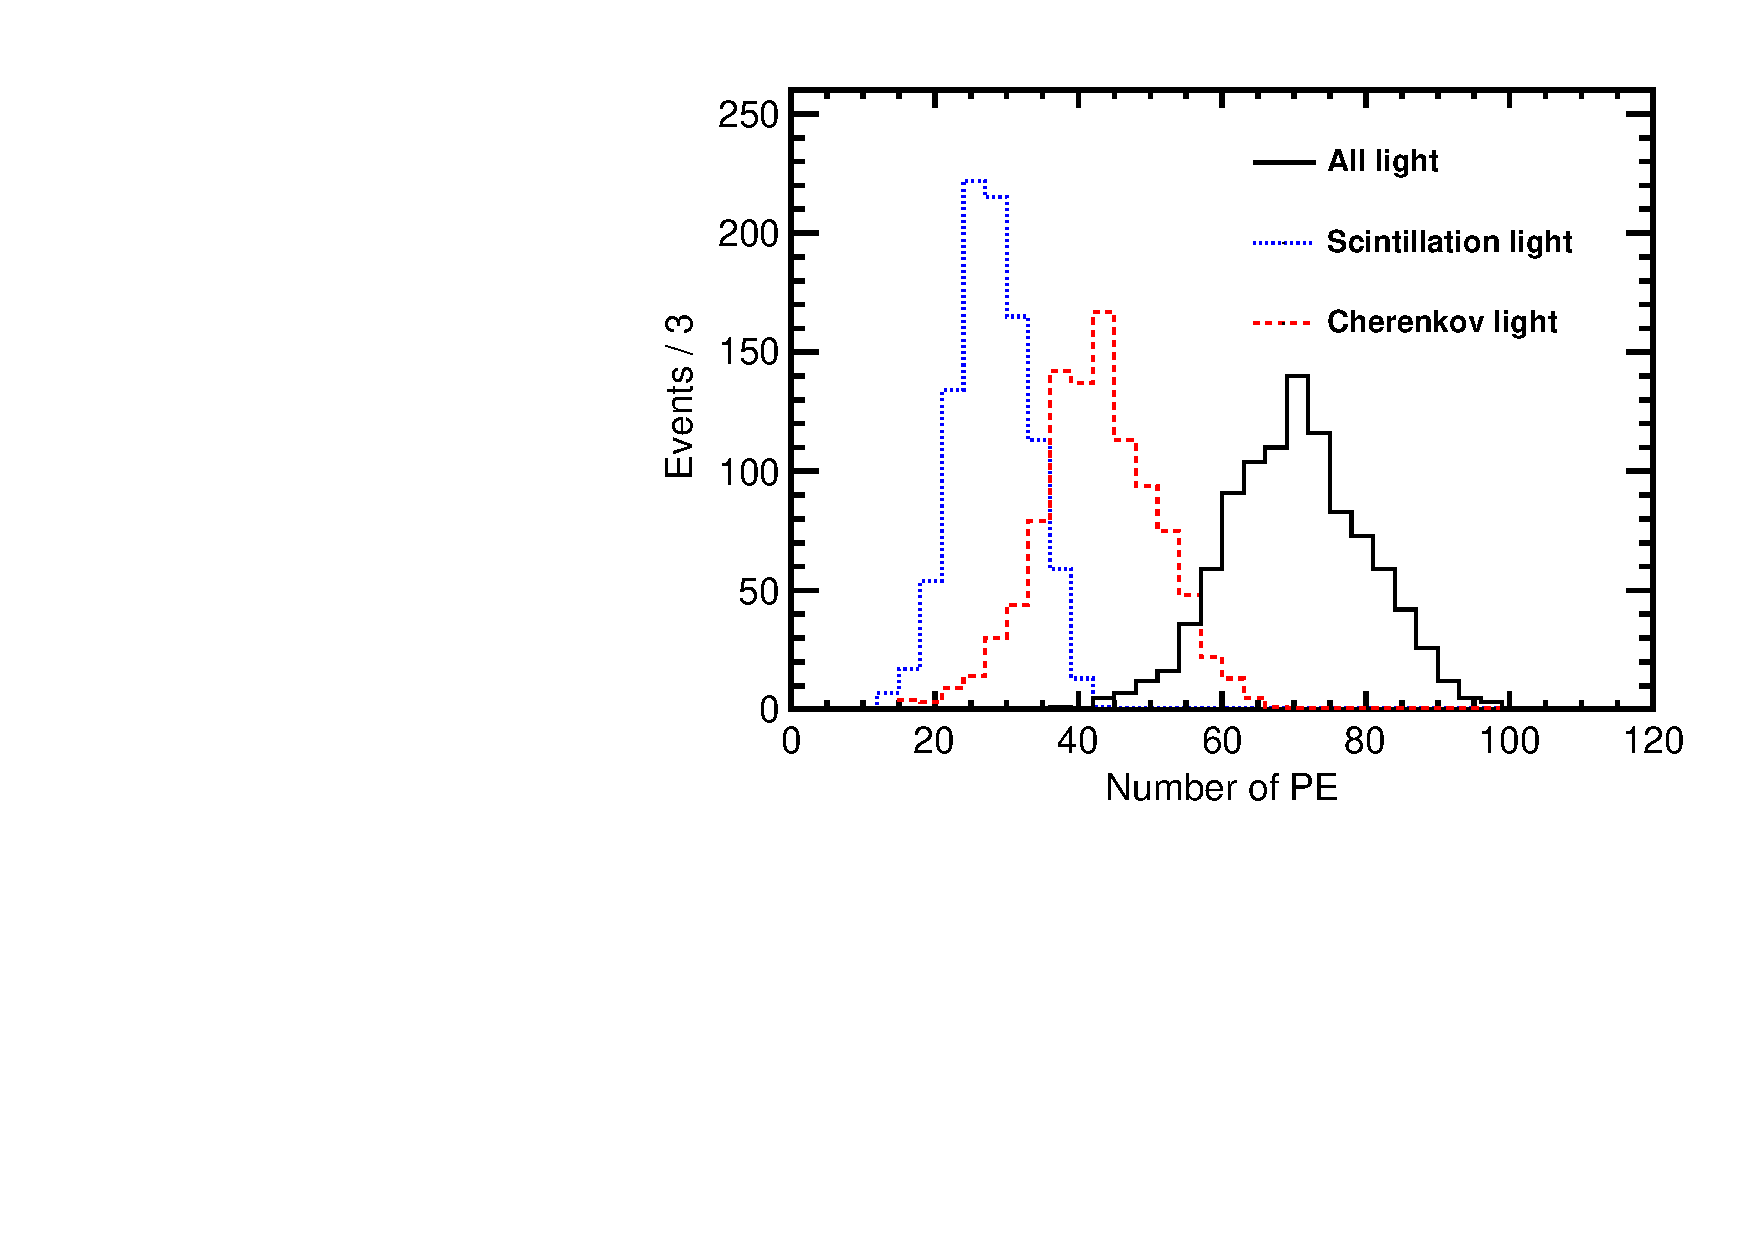
\includegraphics[width=0.45\textwidth]{hMomNPhot_1el_2p529MeV.pdf}
  \caption{Number of Cherenkov (\emph{dashed red line}), scintillation
    (\emph{dotted blue line}), and total (\emph{solid black line}) PEs
    for the simulation of 1000 $^{130}$Te 0{\nbb} decay (left panel)
    and $^8$B (\emph{right panel}) events.}
\label{fig:NPhotDist}
\end{figure*}


\clearpage %These are only needed to force correct placement of the
           %figures while there is no text

\section{Event Topology and the Spherical Harmonics Analysis}
\label{sec:topology_and_harmonics}

We have developed a method based on a spherical harmonics
decomposition to discriminate the topologies of 0\nbb-decay
two-electron events and \B-neutrino single-electron events. The
identification of the Cherenkov photon clusters is challenging due to
the smearing of the characteristic ring pattern by multiple scattering
of the electrons and by the smallness of the Cherenkov signal
relative to the large amount of uniformly-distributed scintillation
light.  We find that performing the spherical harmonics analysis on
the smaller early PE sub-sample, which has a relatively high fraction
of Cherenkov PEs, can discriminate 0\nbb-decay signal events from
backgrounds, although a high rejection factor will require a slower
scintillator than in the model.

\subsection{Topology of 0\nbb-decay and \B~Events}
\label{subsec:topology}

With \Te as the active isotope, all background from \B~solar neutrinos
will have the single electron above Cherenkov threshold in the liquid
scintillator. Also, a large fraction of 0\nbb-decay signal events will
have both electrons above Cherenkov threshold.

In some cases only one Cherenkov cluster is produced in 0\nbb-decay
signal events. This happens either when the angle between the two
0\nbb-decay electrons is small and Cherenkov clusters overlap or when
the energy split between electrons is not balanced, causing one
electron to be below Cherenkov threshold.  Such signal events cannot
be separated from background based on the topology of the distribution
of Cherenkov photons on the detector surface.  However, the
directionality of the electron that is above Cherenkov threshold can
still be reconstructed. This directionality information may allow for
suppression of \B~events based on the position of the
sun~\cite{sun_direction_cut}.

For the purpose of illustrating the spherical harmonics analysis
concept, we first consider two distinct topologies: a) two electrons
produced back-to-back at an 180$^{\circ}$ angle;  and b) a single electron.
Figure~\ref{fig:ThreeTopologies_Display_NoMultScat} shows an idealized
simulation of these two topologies for a total electron energy of
2.53~MeV. In order to emphasize ring patterns formed by Cherenkov
photons, the electron multiple scattering process is turned off in this
idealized simulation and a photocathode QE of 30\% is used for both
Cherenkov and scintillation photons. Here the single-electron event
represents an idealized \B~event topology and the two-electron events
represent two special cases of an idealized 0\nbb-decay topology.


\begin{figure*}[h]
  \centering
%  \begin{tabular}{c c c}
  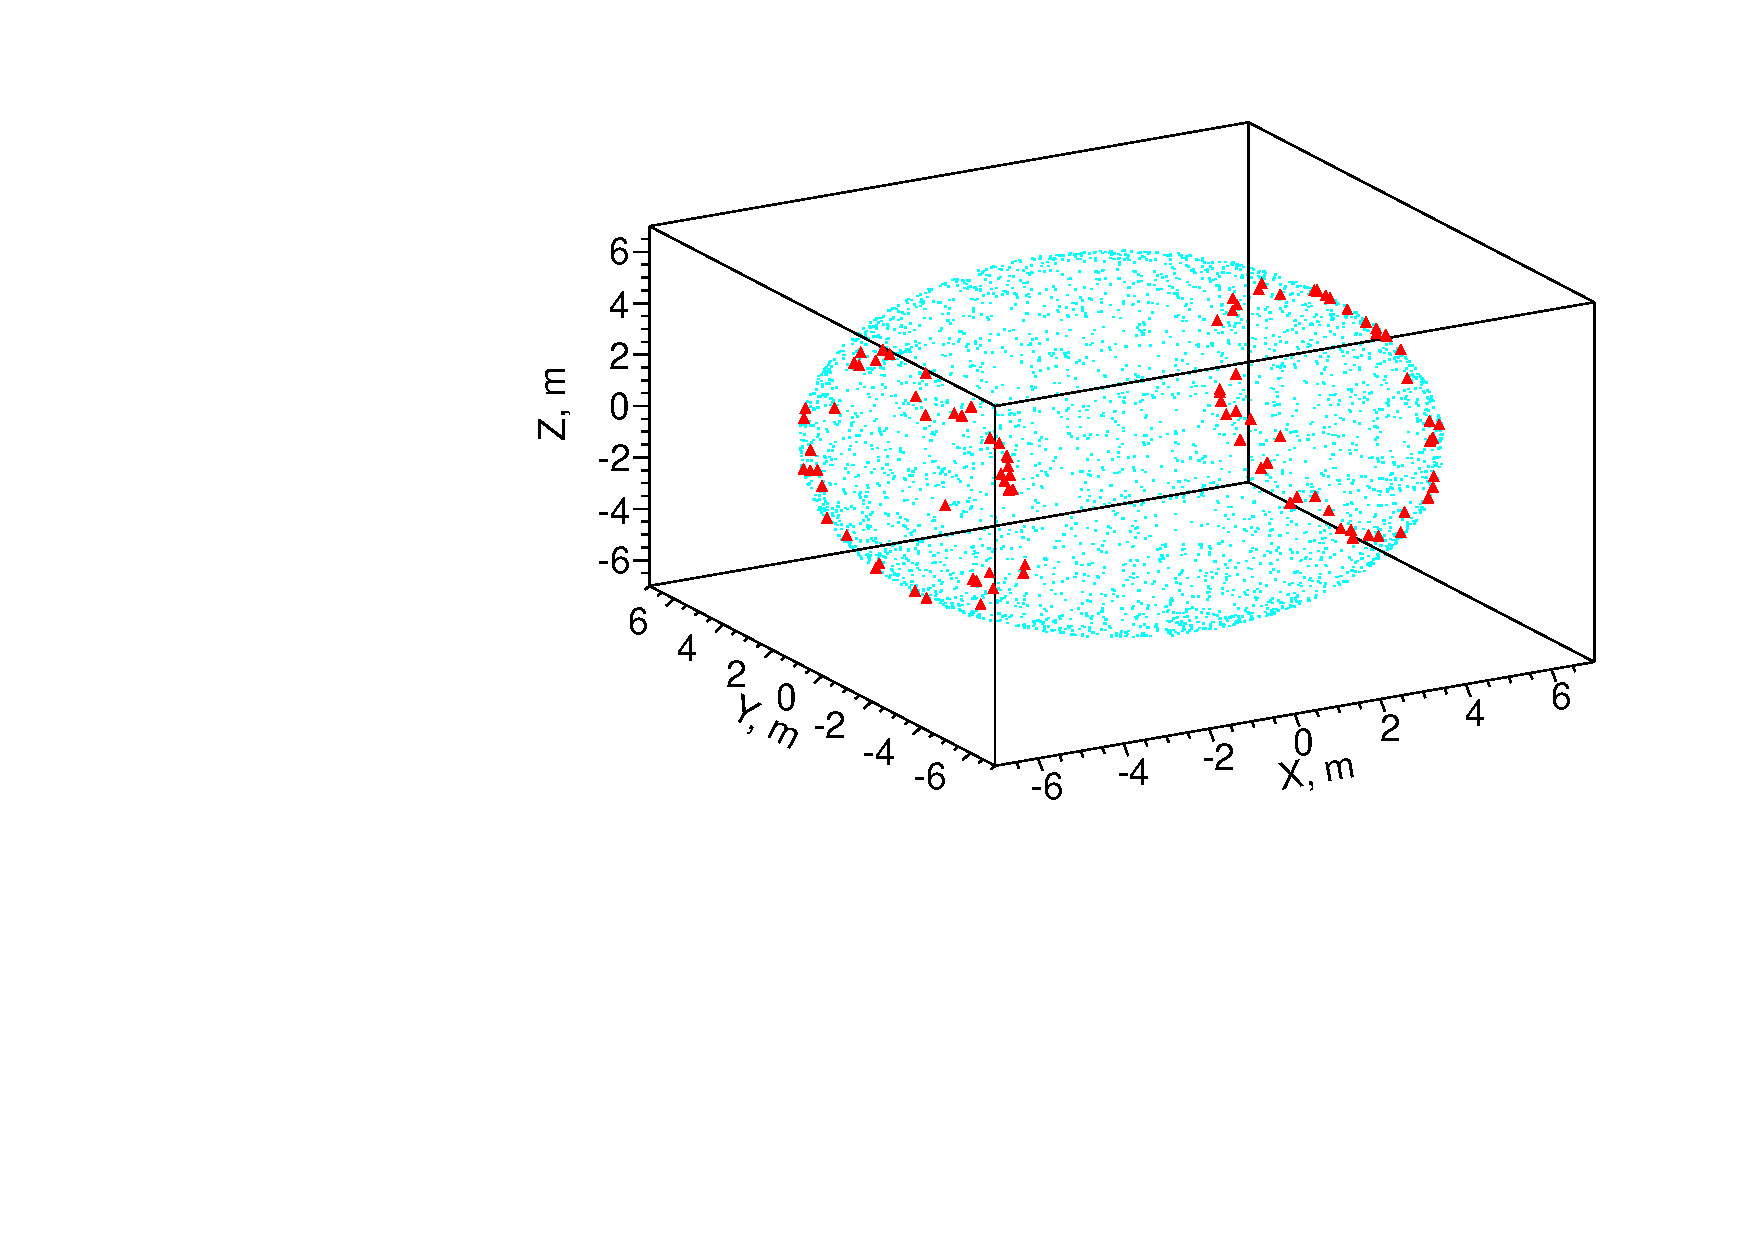
\includegraphics[width=0.45\textwidth]{hDisplay_topology180_NoMultScat.pdf}
%  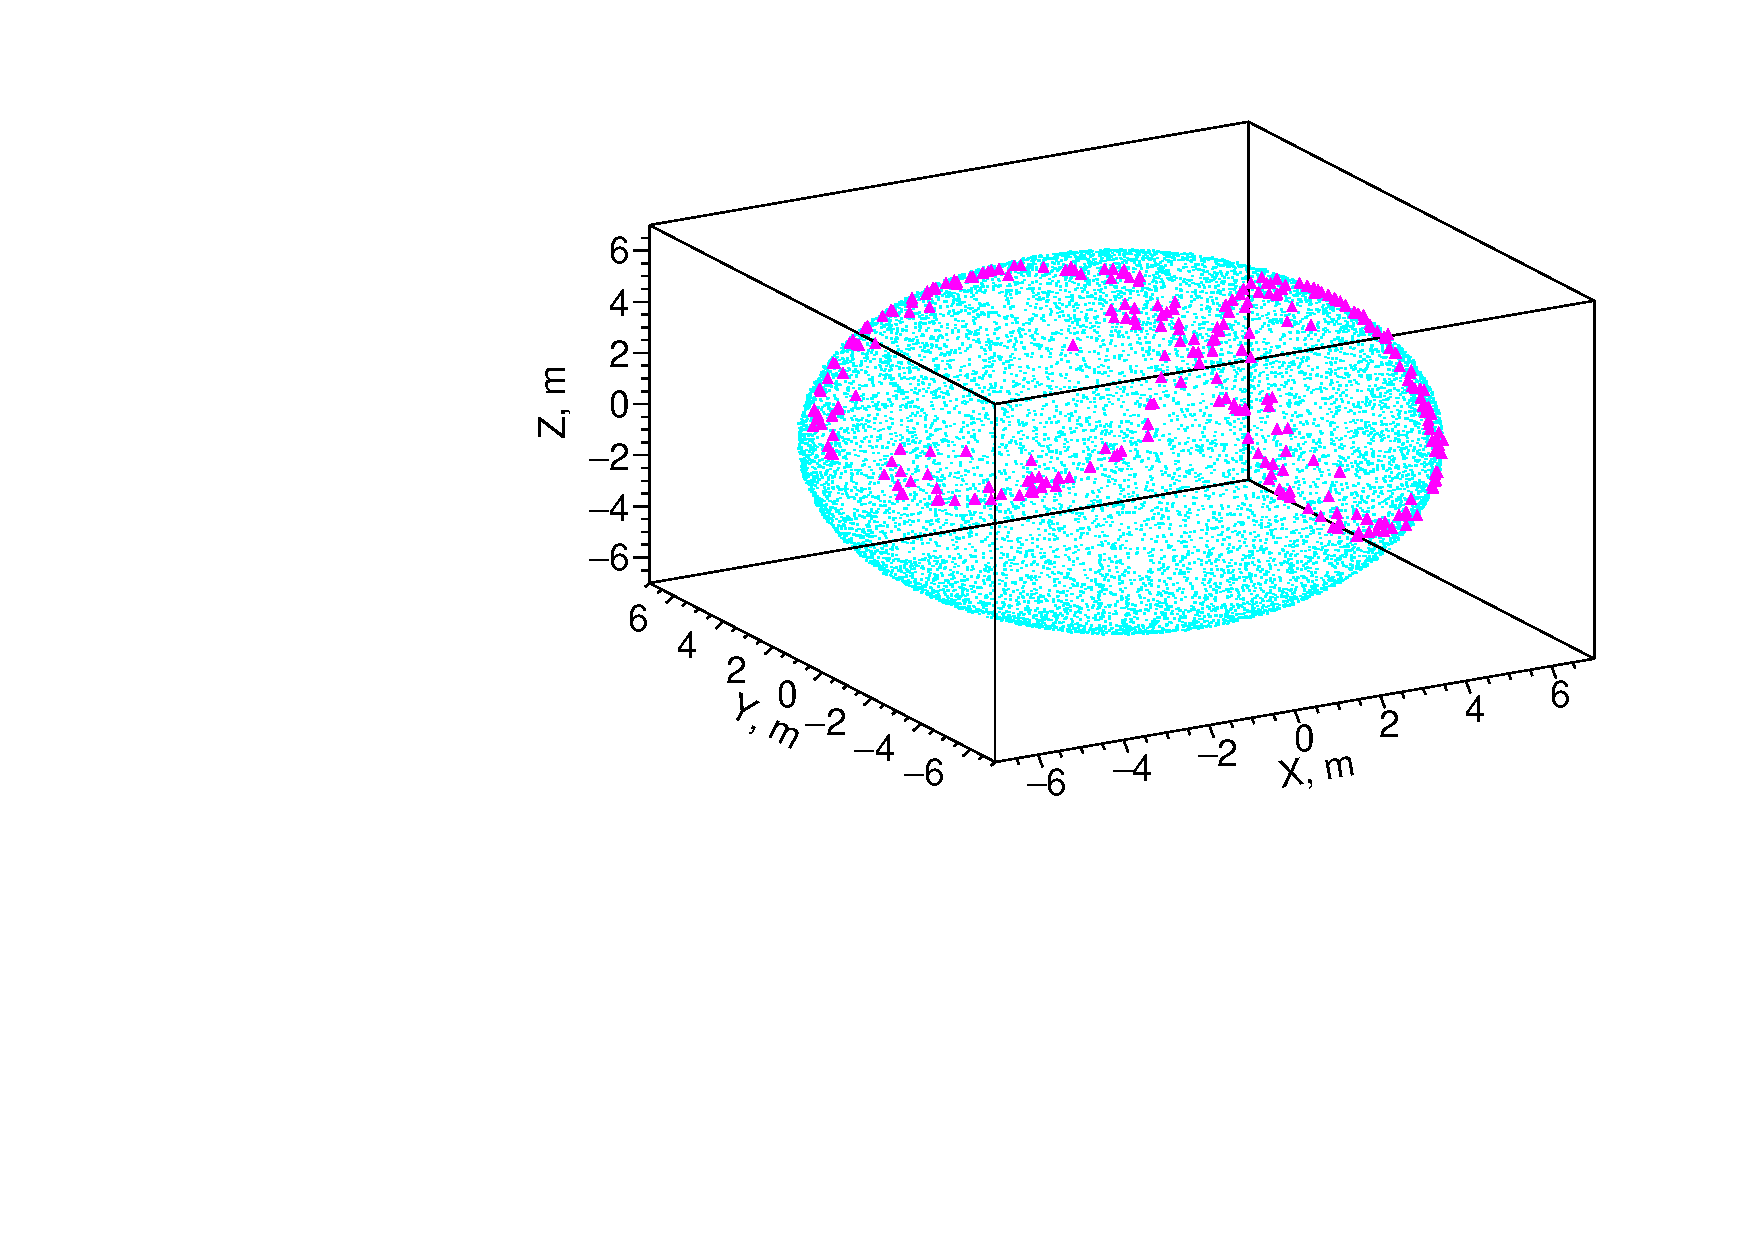
\includegraphics[width=0.33\textwidth]{hDisplay_topology90_NoMultScat.pdf}
  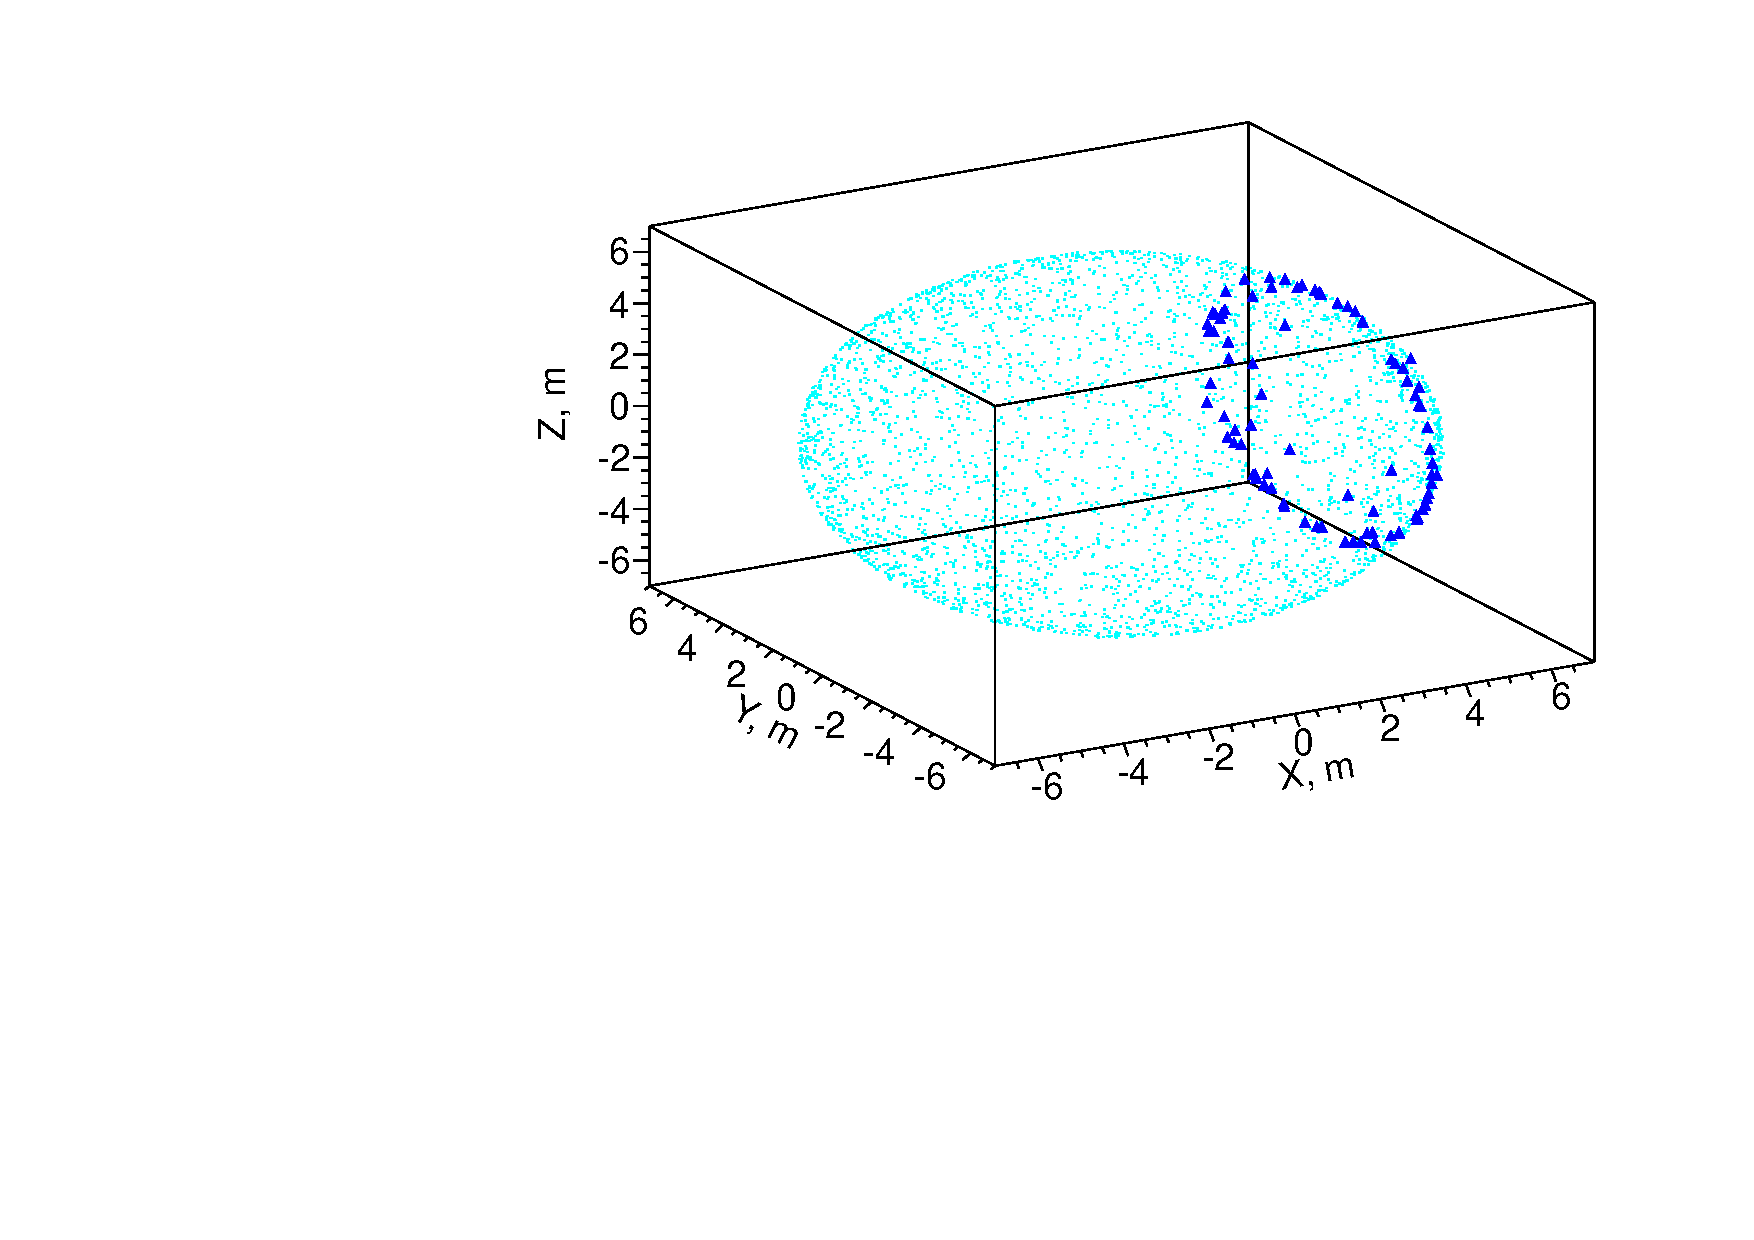
\includegraphics[width=0.45\textwidth]{hDisplay_1el_2p529MeV_NoMultScat.pdf}
%  \end{tabular}
  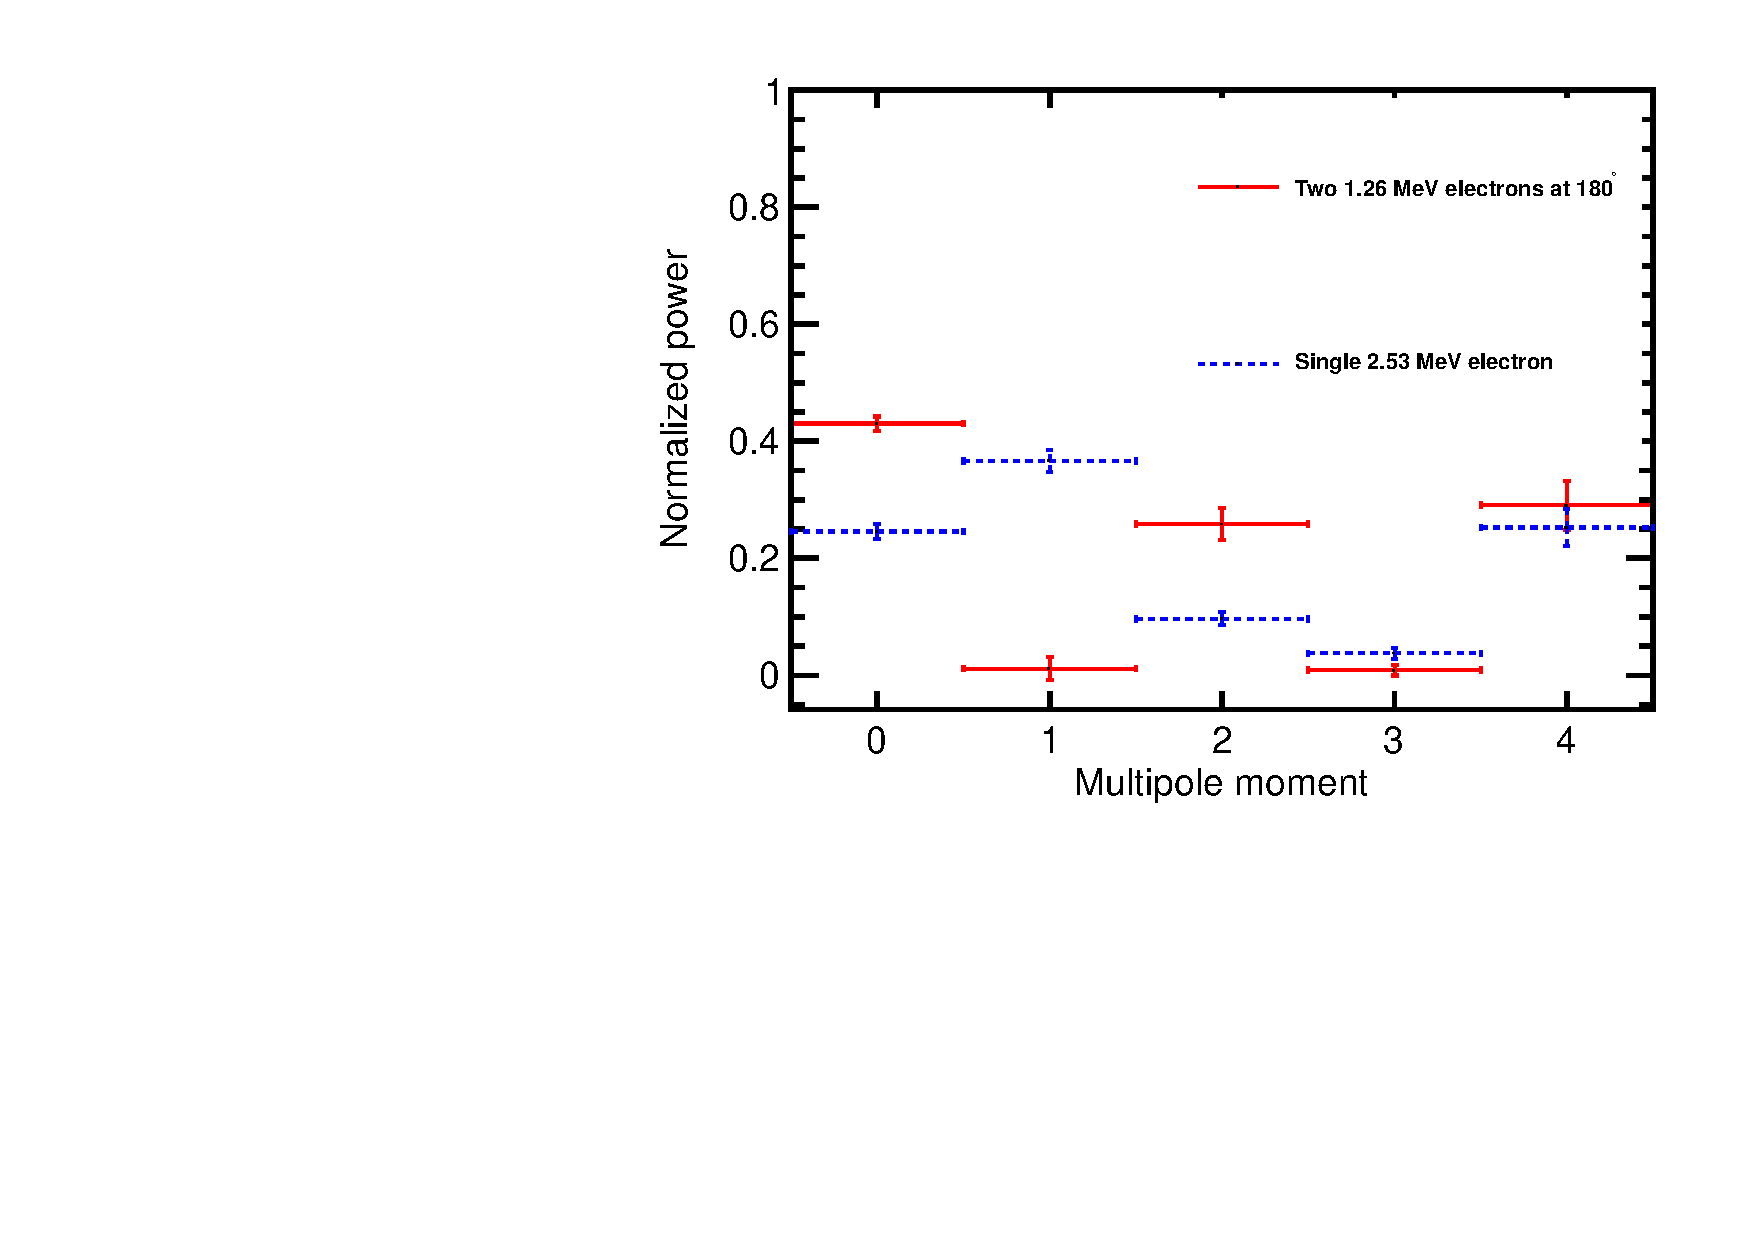
\includegraphics[width=0.9\textwidth]{hMultipleMoment_CHELight_VtxSmear0cm_VtxShiftX0cm_999p9ns_center_NoMultScat.pdf}
  \caption{\emph{Top panels:} Idealized event displays, with multiple
scattering turned off and at the center of the detector, of:
(\emph{top left}) a signal event with two 1.26~MeV back-to-back
electrons; and (\emph{top right })a \B-neutrino background event with
single 2.53~MeV electron. A 30\% QE is assumed for both Cherenkov
photons (triangles) and scintillation photons (dots).  
\emph{Bottom panel:} The normalized power spectrum $S_l$ for the
Cherenkov photons only, calculated event-by-event for the two
above topologies. The height of the rectangular boxes correspond to a 
63\% confidence level $(\pm 1 ~\sigma)$.}
  \label{fig:ThreeTopologies_Display_NoMultScat}
\end{figure*}


\subsection{Description of the Spherical Harmonics Analysis}

The central strategy of the spherical harmonics analysis is to
construct rotationally invariant variables that can be used to
separate different event topologies. To account for the fluctuation of
the number of PEs from event to event, we use a normalized power,
$S_l$, defined in Appendix A.

The bottom panel in Fig.~\ref{fig:ThreeTopologies_Display_NoMultScat}
compares the normalized power spectra for the two representative event
topologies in the idealized case of no multiple scattering and with a 30\%
quantum efficiency for both Cherenkov and scintillation
photons~\cite{QE}. The method gives a good separation between the
two event topologies.

However, at energies relevant to 0\nbb-decay the Cherenkov rings
become very fuzzy due to electron multiple scattering. In most cases,
$\sim$1~MeV electrons produce randomly shaped clusters of Cherenkov
photons around the direction of the electron track.  Examples of \Te~
0\nbb~and \B~events simulated with multiple scattering, but still at
the center of the detector, are shown in Fig.~\ref{fig:Te130_Display}.
\Te~ events are generated based on the phase factors described
in~\cite{Jenni}.  $^{8}$B events are implemented as
monochromatic electrons with the initial direction along the
$x$-axis. The default QEs of 12\% for Cherenkov light and 23\% for
scintillation light have been  applied. Figure~\ref{fig:Te130_Display} shows
early PEs that pass the 33.5~ns time cut. 
% fix the xxs

In this more realistic example, the uniformly distributed
scintillation light makes it difficult to visually distinguish
the event topology. The power spectra shown in the bottom panel of
Fig.~\ref{fig:Te130_Display}~ are different only at $l$=0 and
$l$=1. We use this difference to separate 0\nbb-decay
signal from \B~background events.

\begin{figure*}[hb]
  \centering
  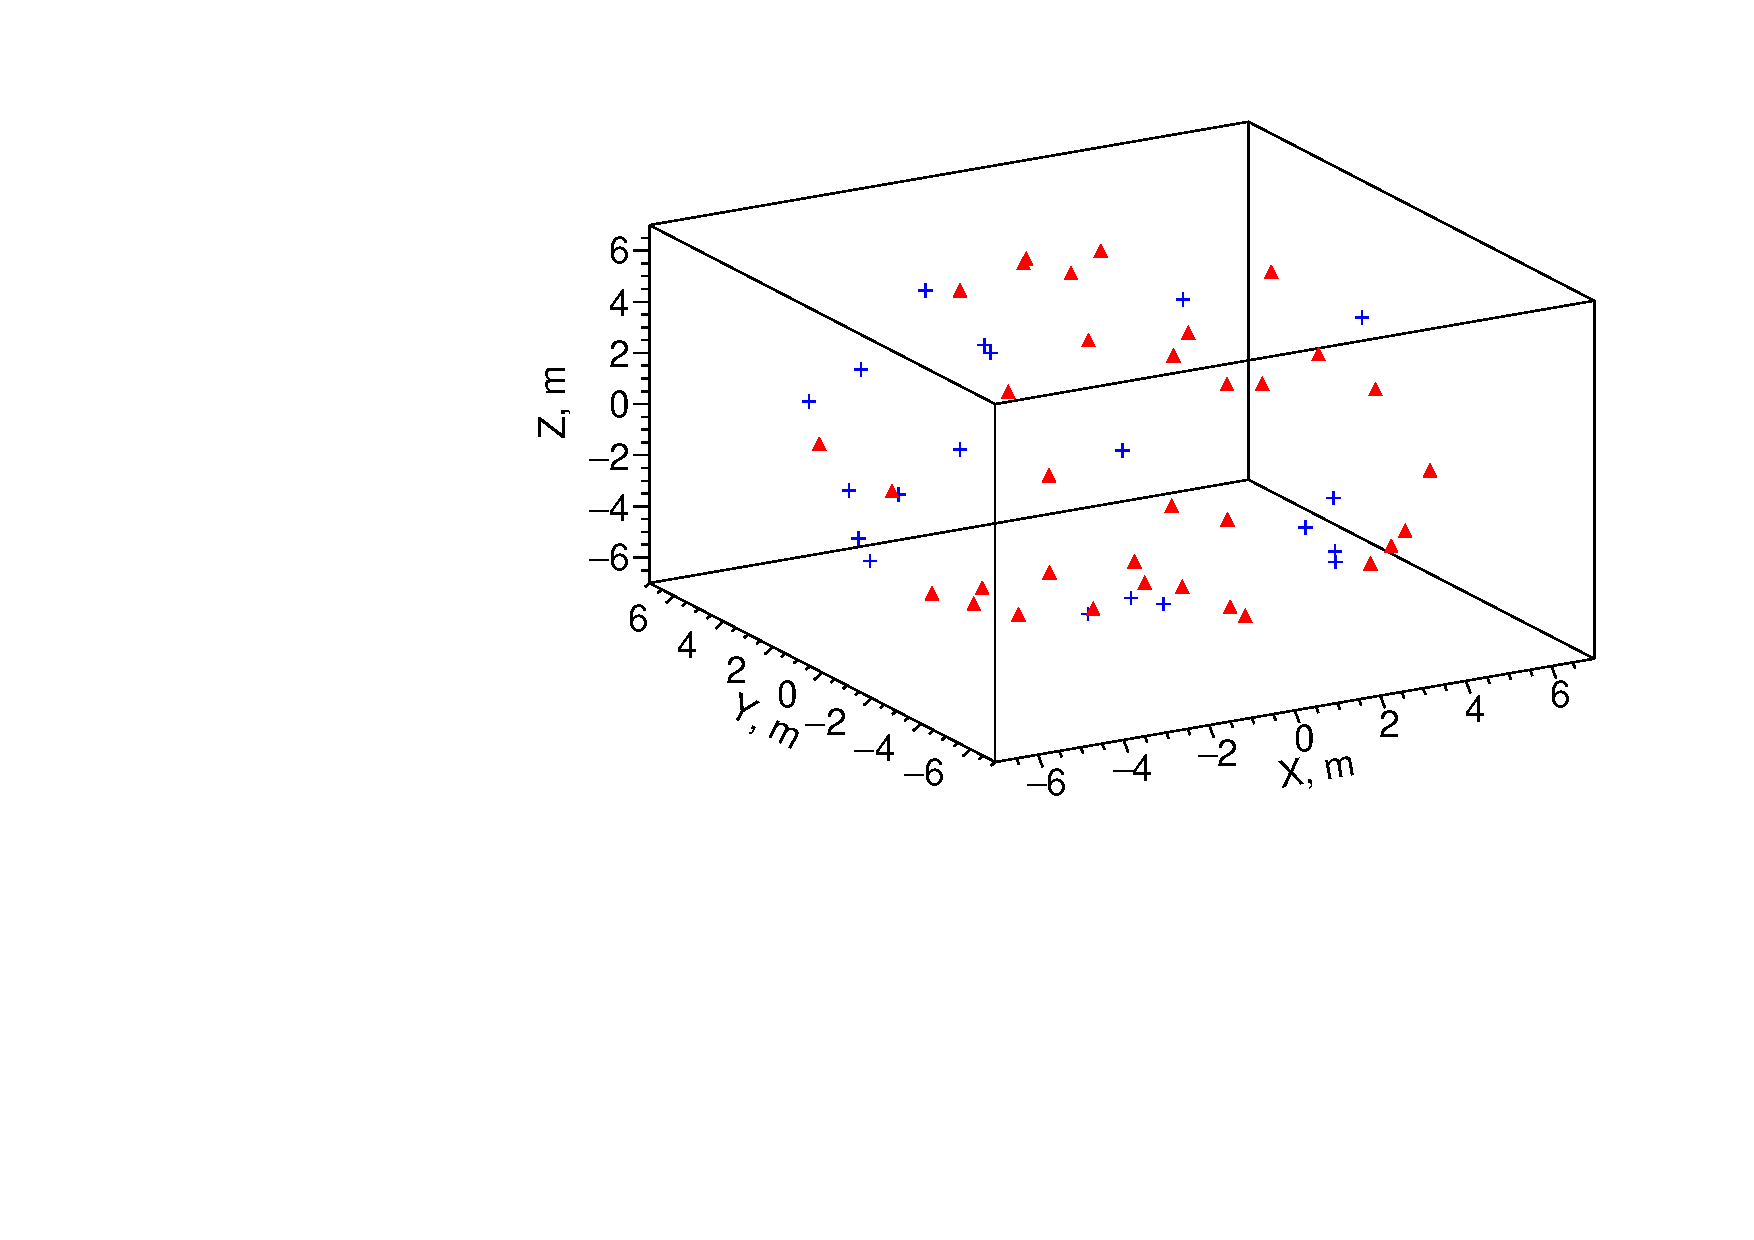
\includegraphics[width=0.42\textwidth]{hDisplay_Te130_evt124_e1257_e1270_cos-0908}
  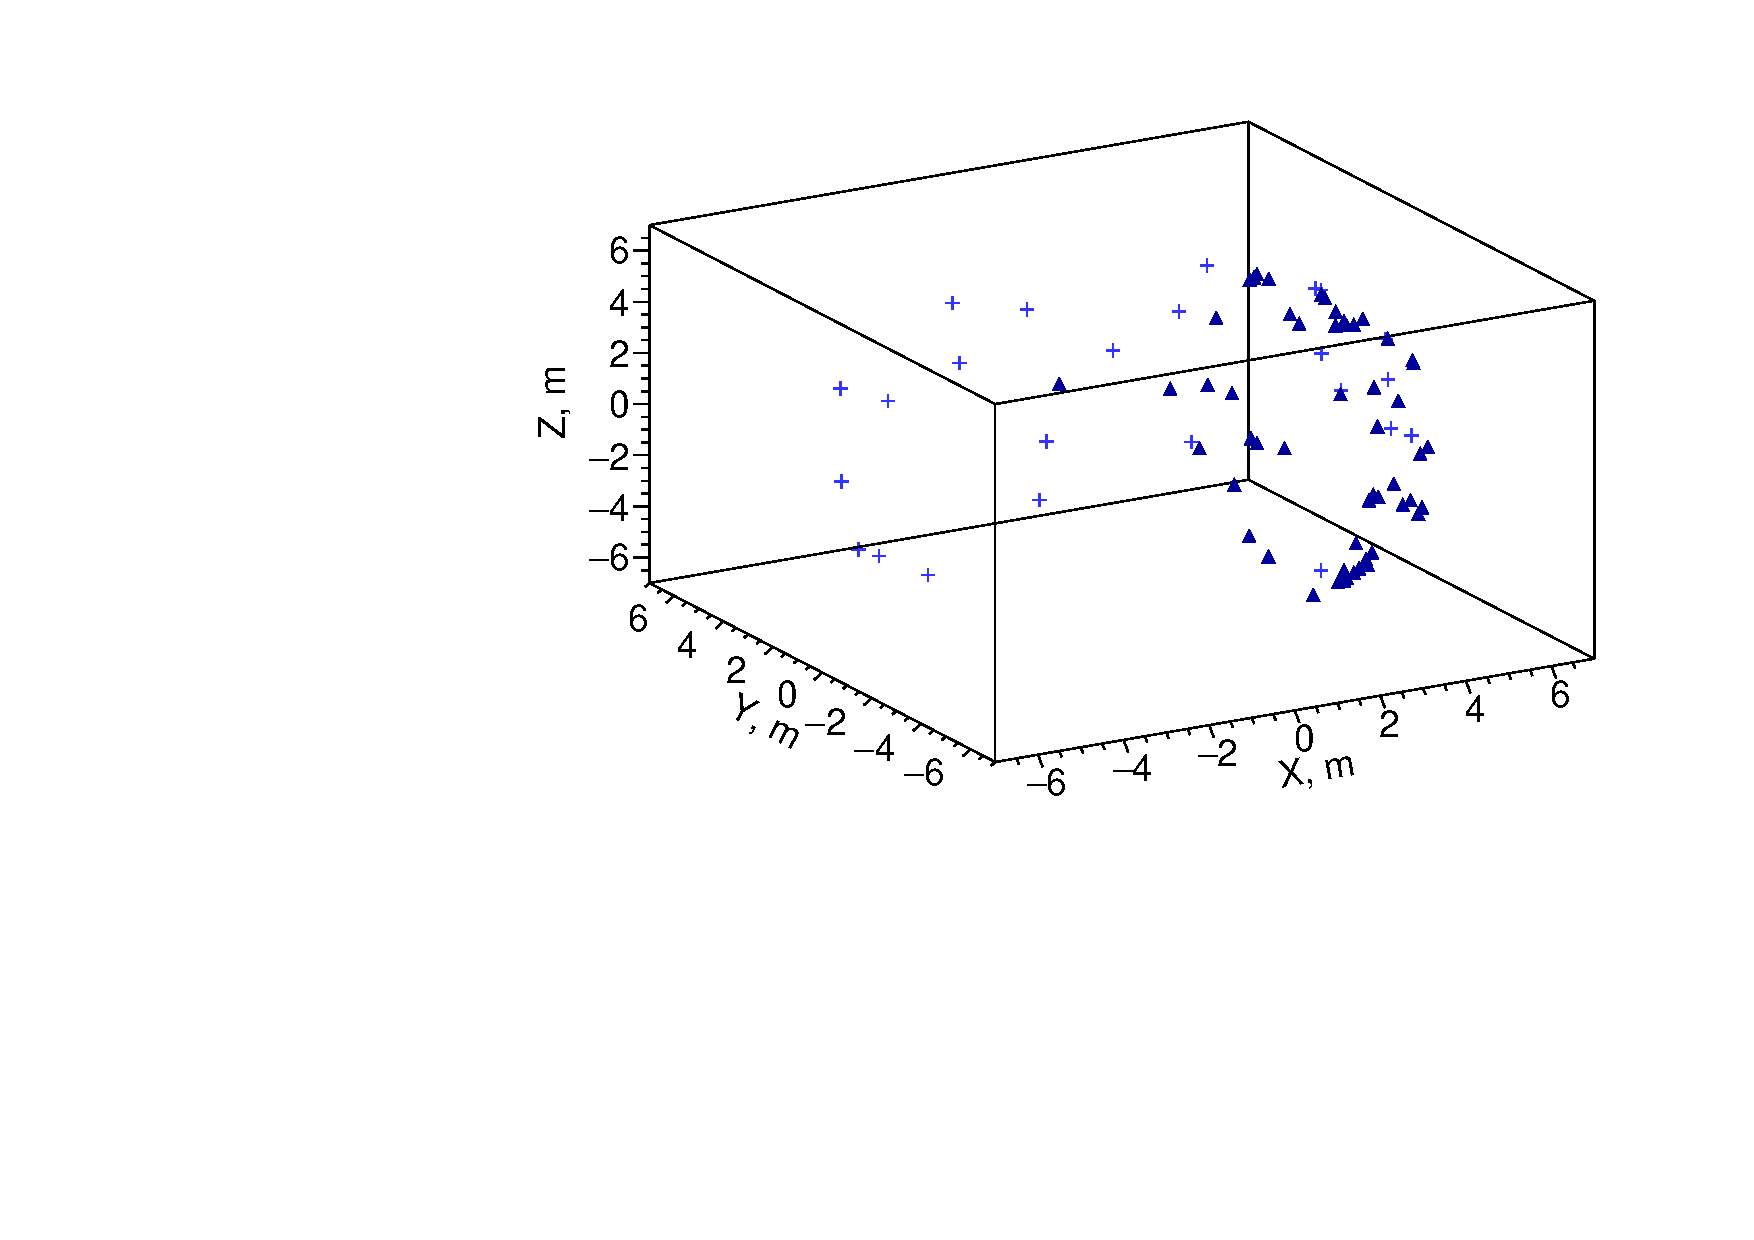
\includegraphics[width=0.42\textwidth]{hDisplay_1el_2p529MeV_33p5ns}
  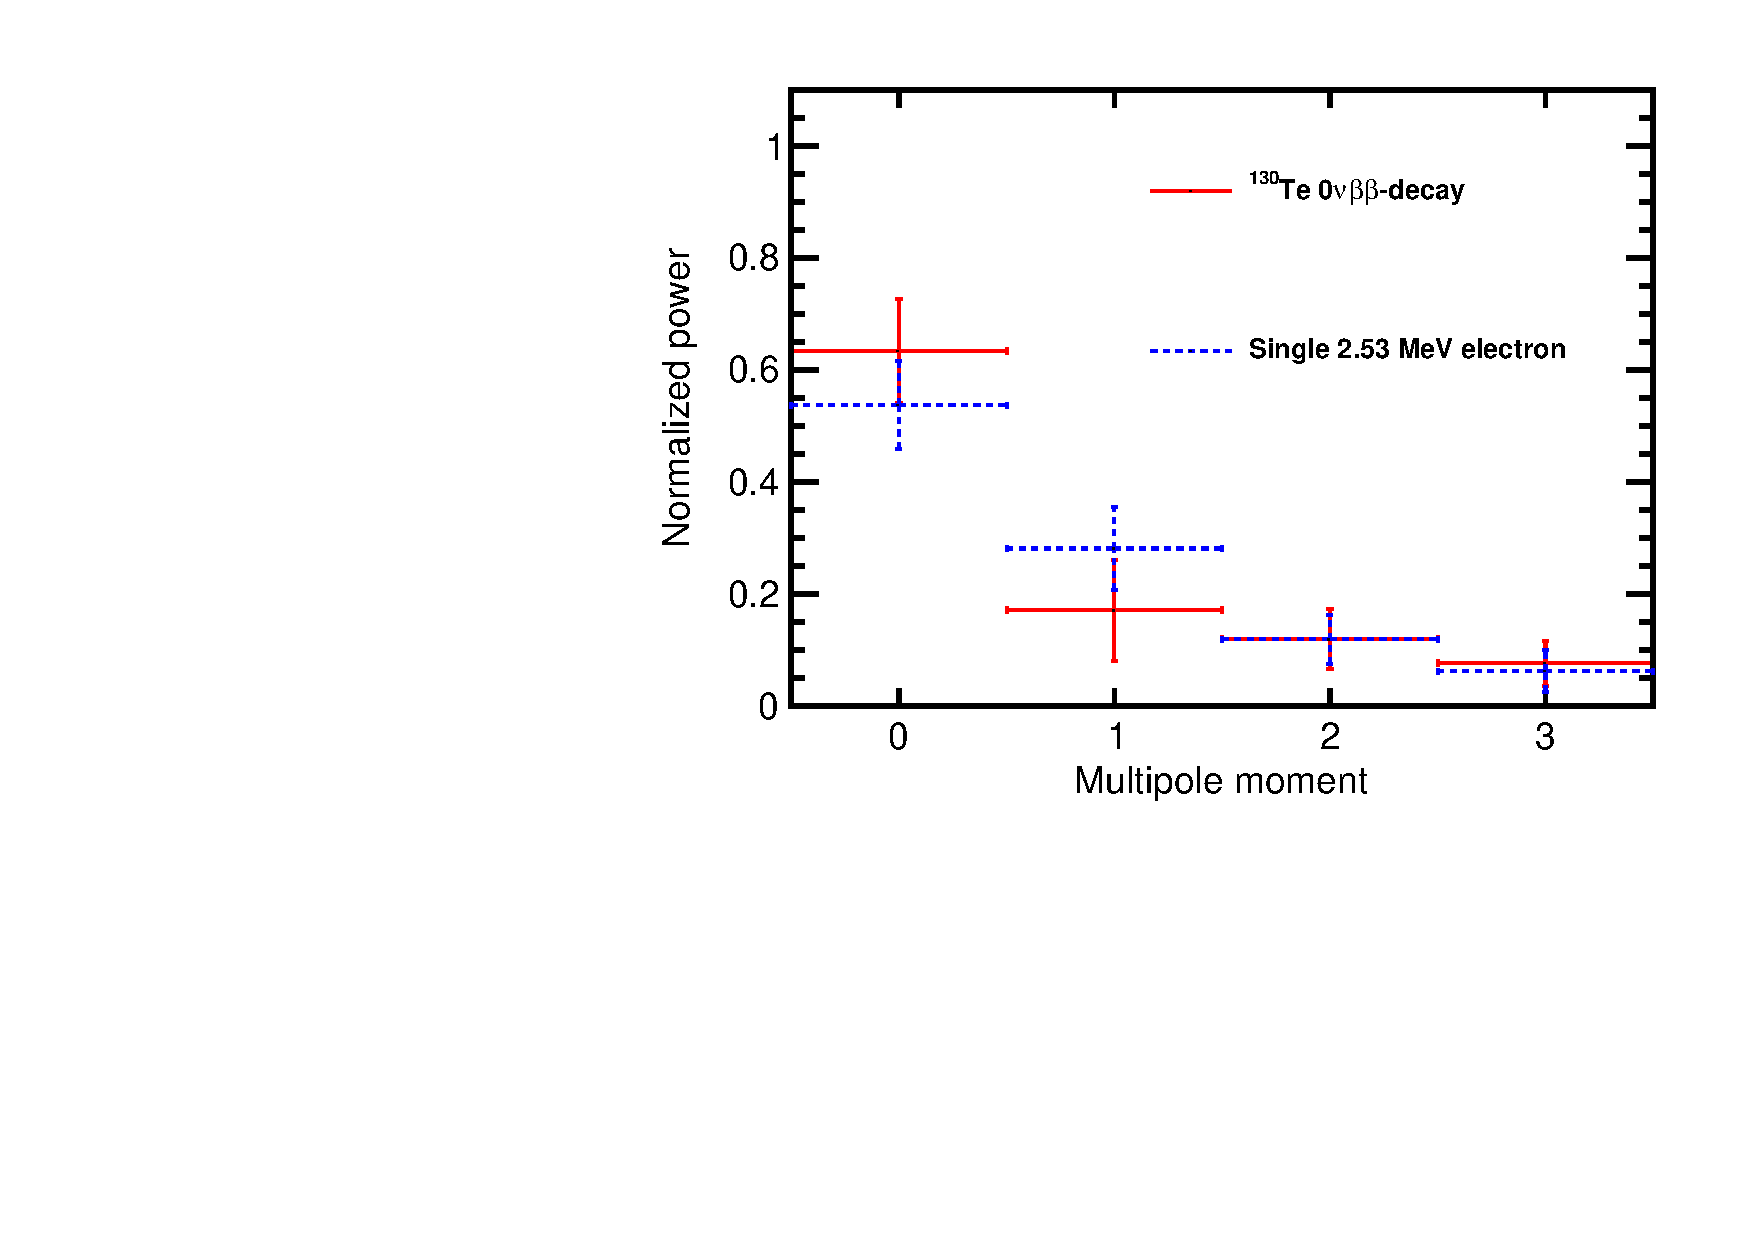
\includegraphics[width=0.8\textwidth]{hMultipleMomentSignal_allLight_VtxSmear0cm_VtxShiftX0cm_33p5ns_center.pdf} 
  \caption{\emph{Top panels:} Event displays with multiple scattering
and at the center of the detector for: (\emph{top left}) a signal
event with two 1.26~MeV back-to-back electrons; and (\emph{top right
})a \B-neutrino background event with a single 2.53~MeV electron. The
model QEs are assumed for both Cherenkov photons (triangles) and
scintillation photons (dots).  \emph{Bottom panel:} The normalized
power spectrum $S_l$ for the Cherenkov photons, calculated
event-by-event for 1000 events of each of the two above topologies. The
heights of the rectangular boxes correspond to a 63\% C.L.
$(\pm 1 ~\sigma)$.}
\label{fig:Te130_Display}
\end{figure*}

We find that 0\nbb~events become indistinguishable from single-track events when
the angle between the two electrons is small and two Cherenkov
clusters overlap. Event topologies of 0\nbb~and \B~events are also
very similar when only one electron from 0\nbb~ is above the Cherenkov
threshold. The spherical harmonics analysis is most efficient
for events with large angular separation between the two electrons and
when both electrons are above Cherenkov threshold~\cite{further_cuts}.




\clearpage %These are only needed to force correct placement of the
           %figures while there is no text

\section{Performance of the Spherical Harmonics Analysis in Separating 0\nbb-decay from \B~Background.}
\label{sec:performance}

In this section we discuss factors that affect performance of the spherical harmonics technique in separating
0\nbb~signal from \B~background events. We found that most separation comes from the first two multiple moments,
$l=0$ and $l=1$. However, according to Eq.~\ref{eq6}, higher multiple moments are needed for a better normalization of the 
power spectrum $S_l$. In the following we choose to calculate power spectrum $s_l$ up to multiple moment of l=3 and
use only normalized variable $S_0$ and $S_1$, where the normalization is given by

\begin{eqnarray}
\label{eq7}
S_{0,1} = \frac{s_{0,1}}{\sum_{l=0}^{3} s_l}
\end{eqnarray}

As discussed below, a linear combination of $S_0$ and $S_1$ can be used to construct a single variable, $S_{01}$, that provides 
separation between signal and background in 1D space. We show distributions of this variable $S_{01}$ to demonstrate qualitatively 
the separation between 0\nbb~and \B~events depending on a few key assumptions about the detector characteristics.

Since the goal of this paper is to describe the technique of spherical harmonics analysis for separating
different event topologies relevant for 0\nbb-decay searches in a generic liquid scintillator detector, we intentionally refrain from any 
quantitative estimates on the improvements in sensitivity to 0\nbb~decay. The actual improvements in sensitivity due to spherical 
harmonics analysis would depend on various details of a given experimental setup. Therefore, we believe that detailed qunatitative 
sensitivity studies are more apporpiate in the context of a particular 0\nbb~decay experiment which is beyond the scope of this paper.

\subsection{Central events with perfect vertex reconstruction}

We start evaluating the performance of the sphercical harmonics analysis from looking into events that originate at the center
of the detector and assuming perfect reconstruction of the event vertex position. For such events, a time cut of 33.5~ns on PEs 
arrival time can be applied to obtain early PEs sample which contain high fraction of Cherenkov PE. The default QE and 100\% 
photo-coverage is used in the simulation.

Comparison of $S_0$ and $S_1$ distributions for 0\nbb-decay signal and \B~background events is shown in Fig.~\ref{fig:S_vs_energy}.
Both variables provide a noticeable separation between signal and background. We also note that in the energy range of interest, 
the $S_l$'s do not strongly depend on the energy deposited in the detector, which makes information contained in the normalized power 
spectrum complimentary to the energy measurements. Therefore, spherical harmonics analysis can be used as an additional handle for
background suppresion at the end point of the 0\nbb-decay energy spectrum.

\begin{figure*}[h]
\centering
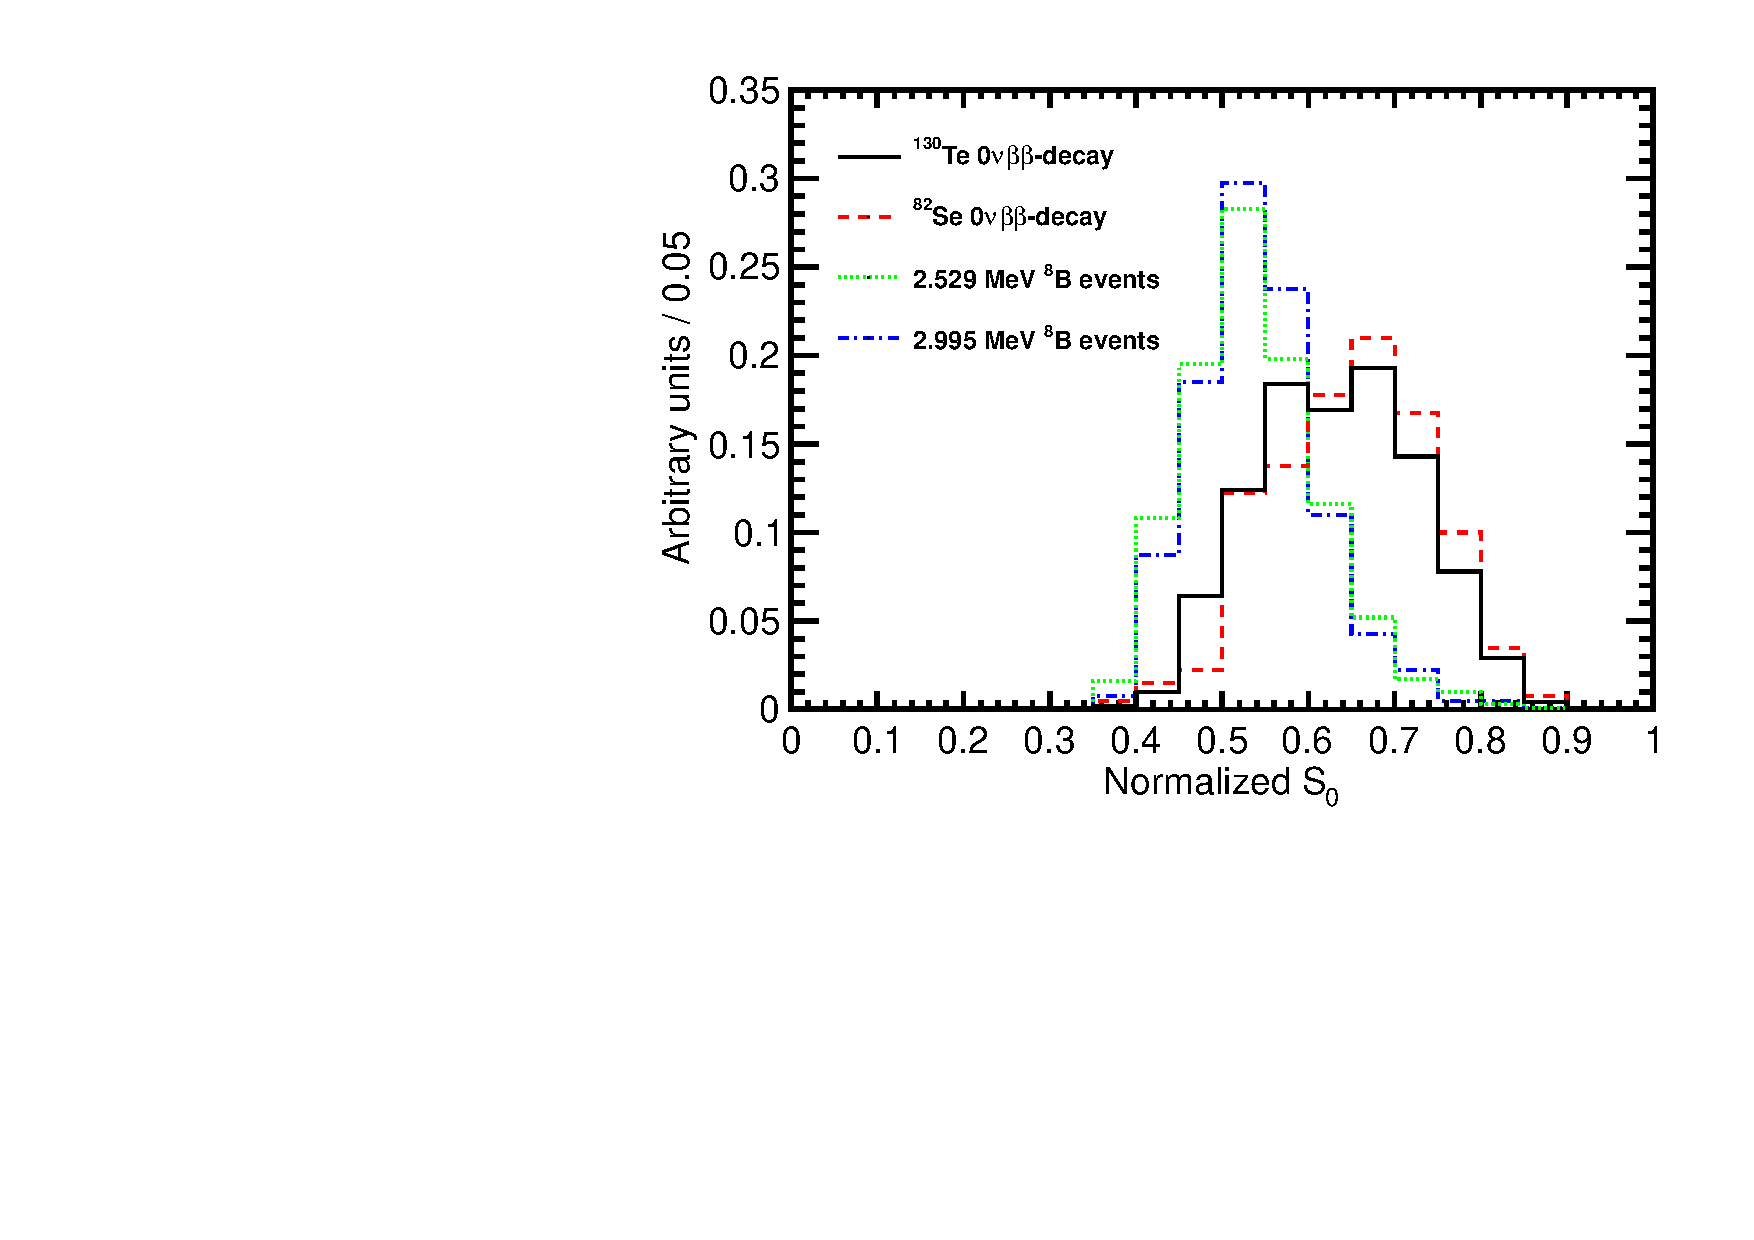
\includegraphics[width=0.49\textwidth]{hS0.pdf}
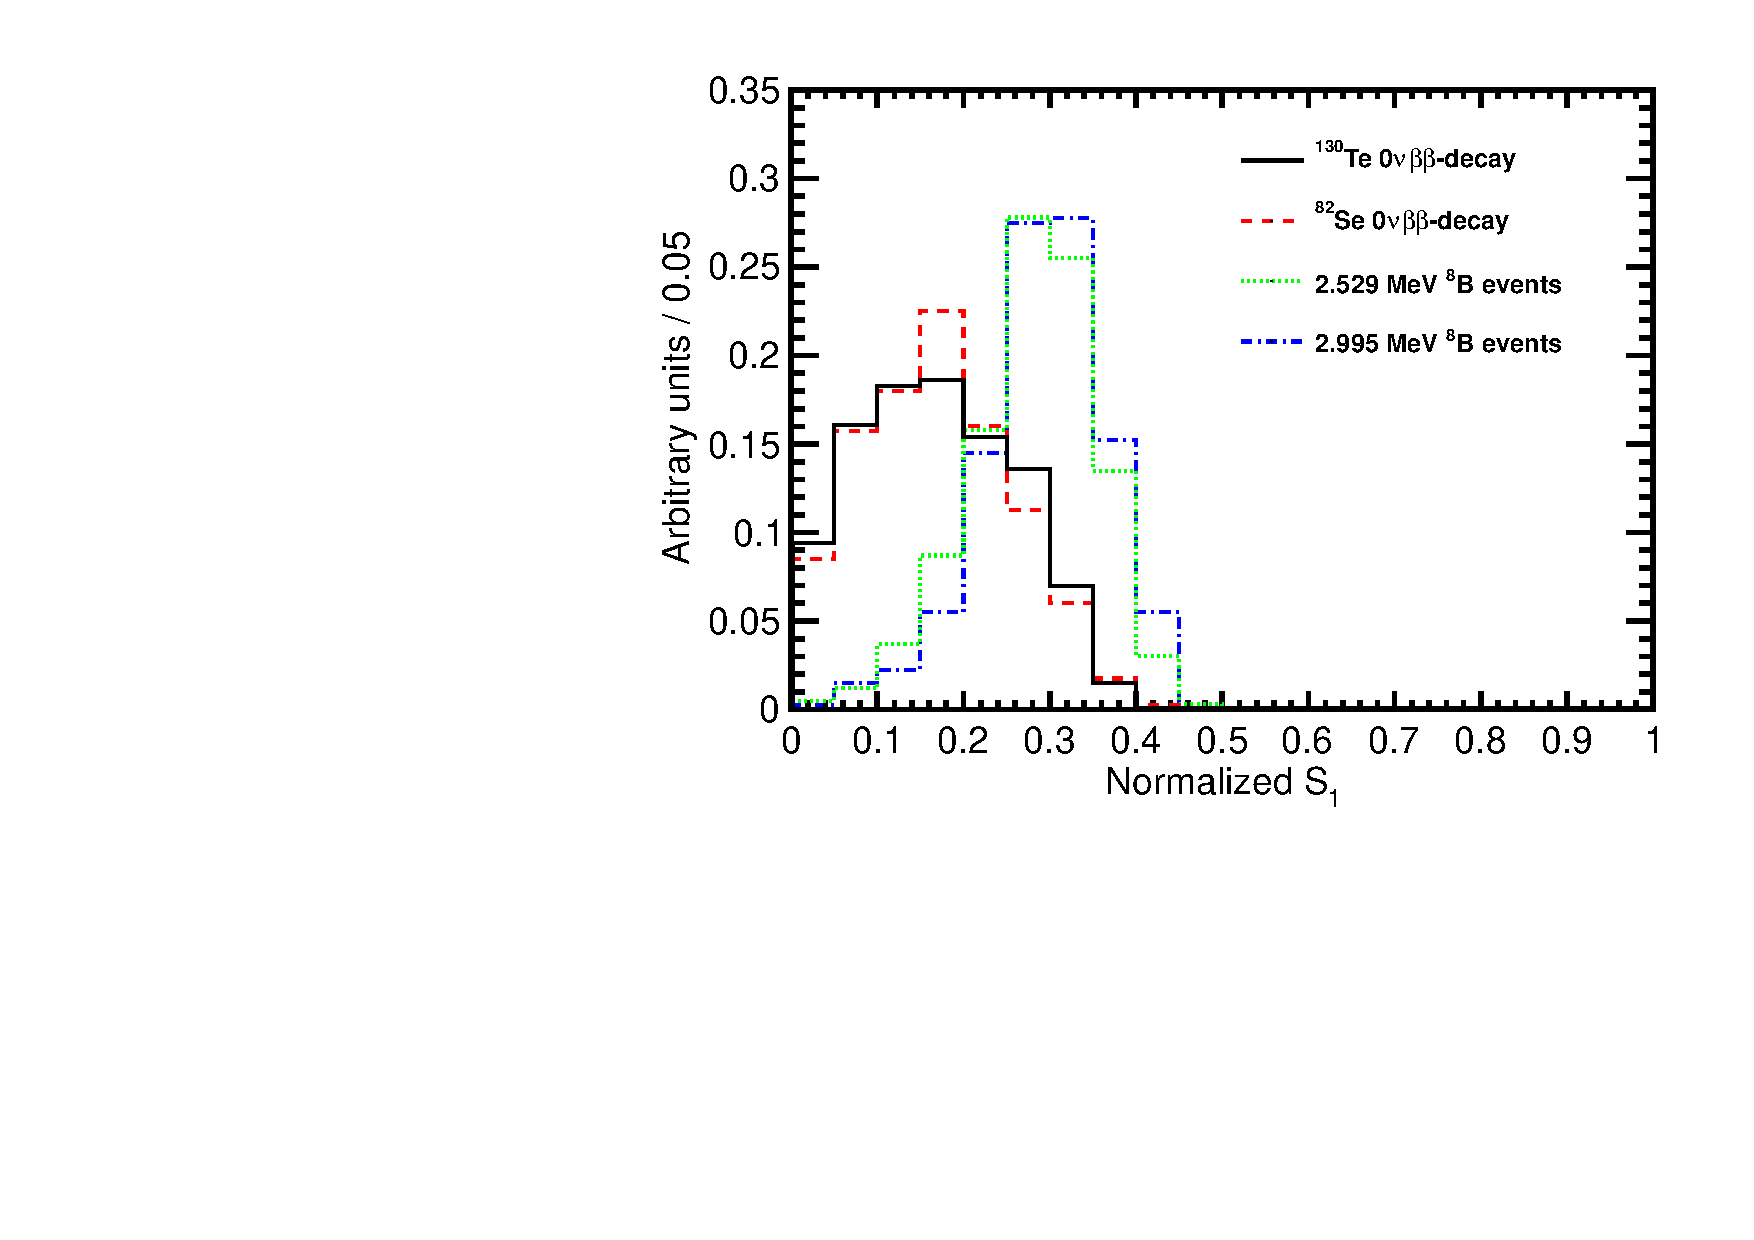
\includegraphics[width=0.49\textwidth]{hS1.pdf}
\caption{$S_0$ (\emph{left}) and $S_1$ (\emph{right}) distributions for 1000 simulated 0\nbb-decay signal and \B~background events.
  Two different isotopes are compared, $^{130}$Te and $^{82}$Se. Corresponding kinetic energies of \B~single electrons are
  2.53 MeV and 3.00 MeV. Central events assuming perfect reconstruction of vertex position. Time cut of 33.5~ns on the PE arrival time is
  applied. The default QE and 100\% photo-coverage is used in the simulation.}
\label{fig:S_vs_energy}
\end{figure*}

Left panel in Fig.~\ref{fig:SL_Te_33p5ns_center} compares scatter plots of the first two components of the power spectrum, 
$S_0$ and $S_1$, for signal and background. In order to optimize separation between $^{130}$Te and $^{8}$B
events, a linear combination of $S_0$ and $S_1$, $S_{01}$, is constructed as follows. 

First, a linear fit, $S_0$ = $A \cdot S_1 + B$, of all points on the scatter plot is performed as shown by the dashed 
line in the left panel of Fig.~\ref{fig:SL_Te_33p5ns_center}. Then a 1-D variable $S_{01}$ is defined as
$S_{01} = S_1 \cdot cos(\theta) + S_0 \cdot sin(\theta)$, where $tan(\theta)$=$A$. Right panel in Fig.~\ref{fig:SL_Te_33p5ns_center}
compares distributions of $S_{01}$ for 0\nbb-decay signal and \B~background. These 1-D histogrmas for $S_{01}$ represent
projection of points on the scater plot onto the fitted line. We use distribution of the variable $S_{01}$ as a figure of merit
for signal/background separation. We conclude that spherical harmonics analysis potentialy brings new separation power that is
in addition to energy measusrements.


\begin{figure*}[h]
  \centering
  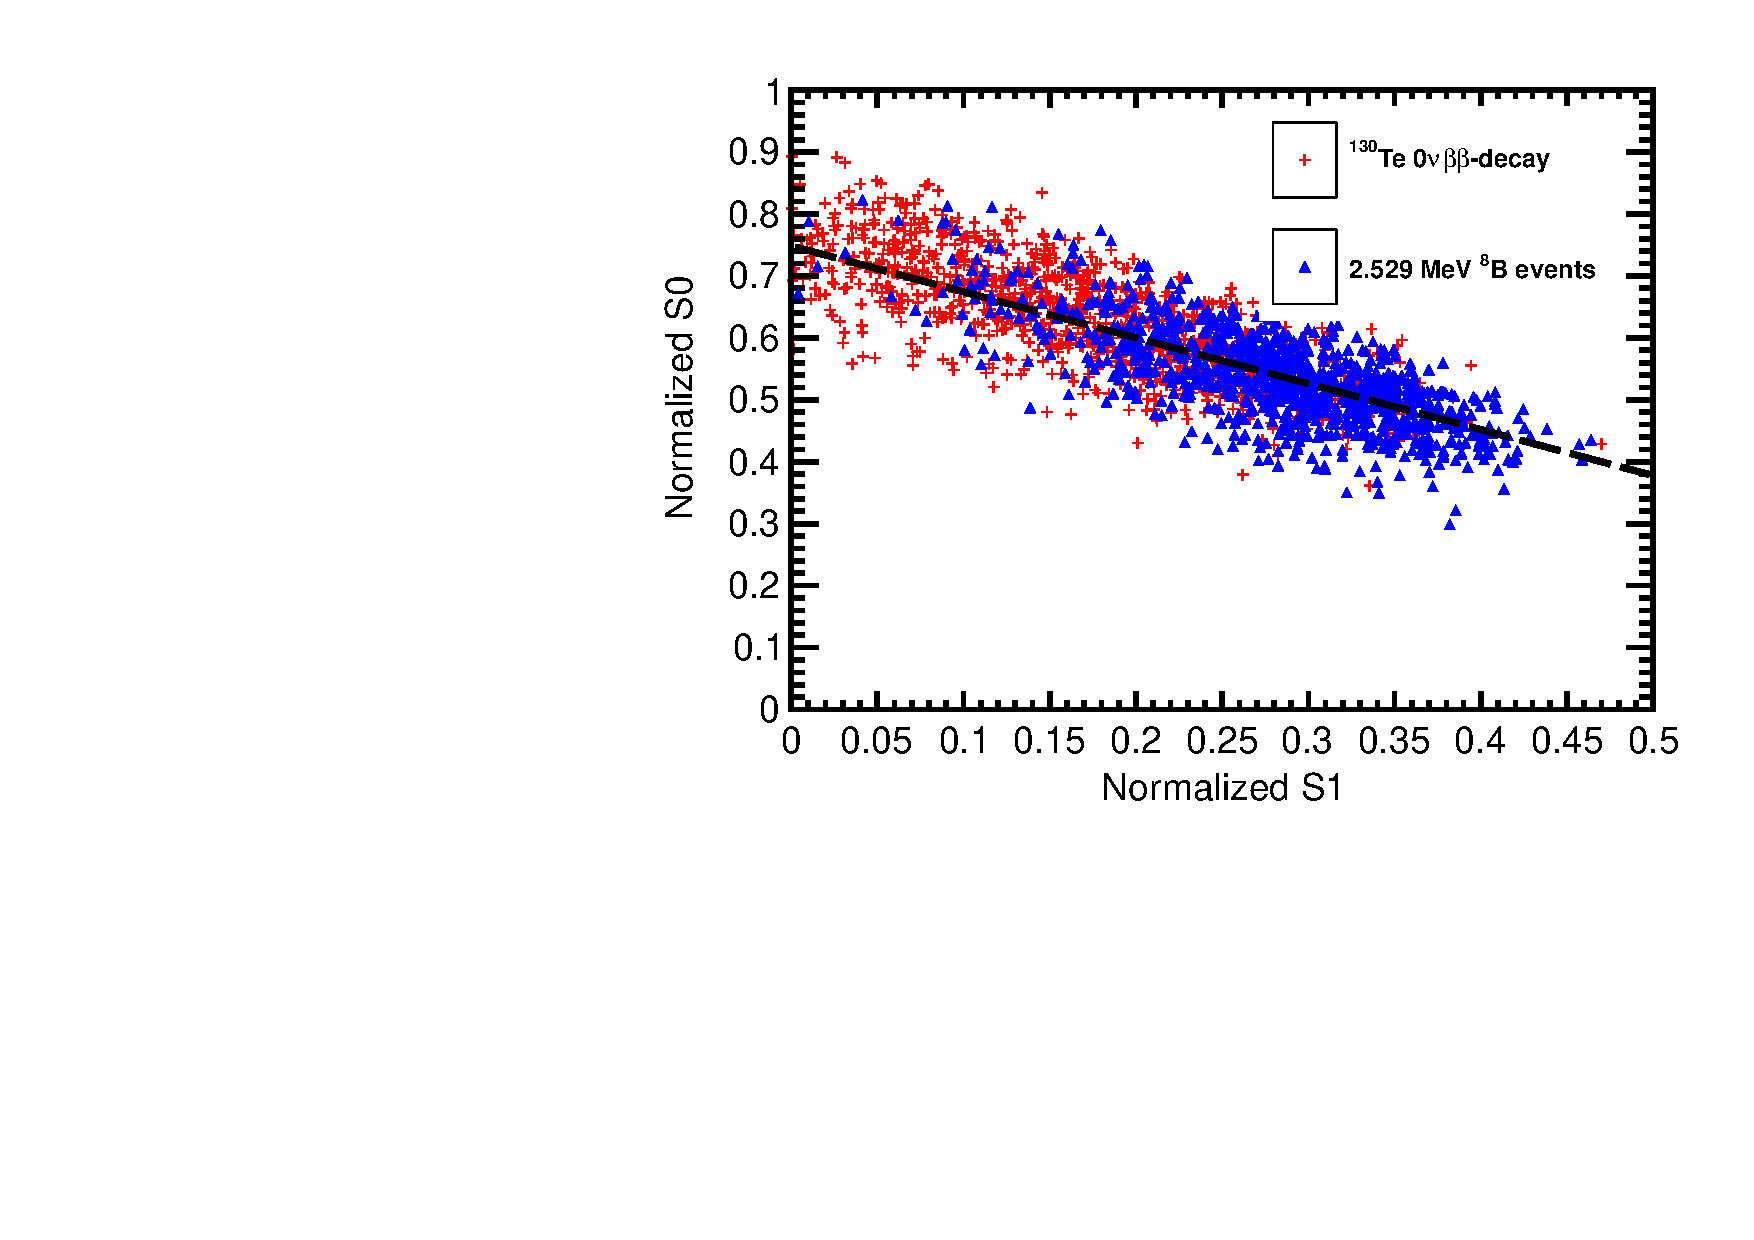
\includegraphics[width=0.49\textwidth]{hS0vsS1_Te130_1el_allLight_VtxSmear0cm_VtxShiftX0cm_33p5ns_center.pdf}
%  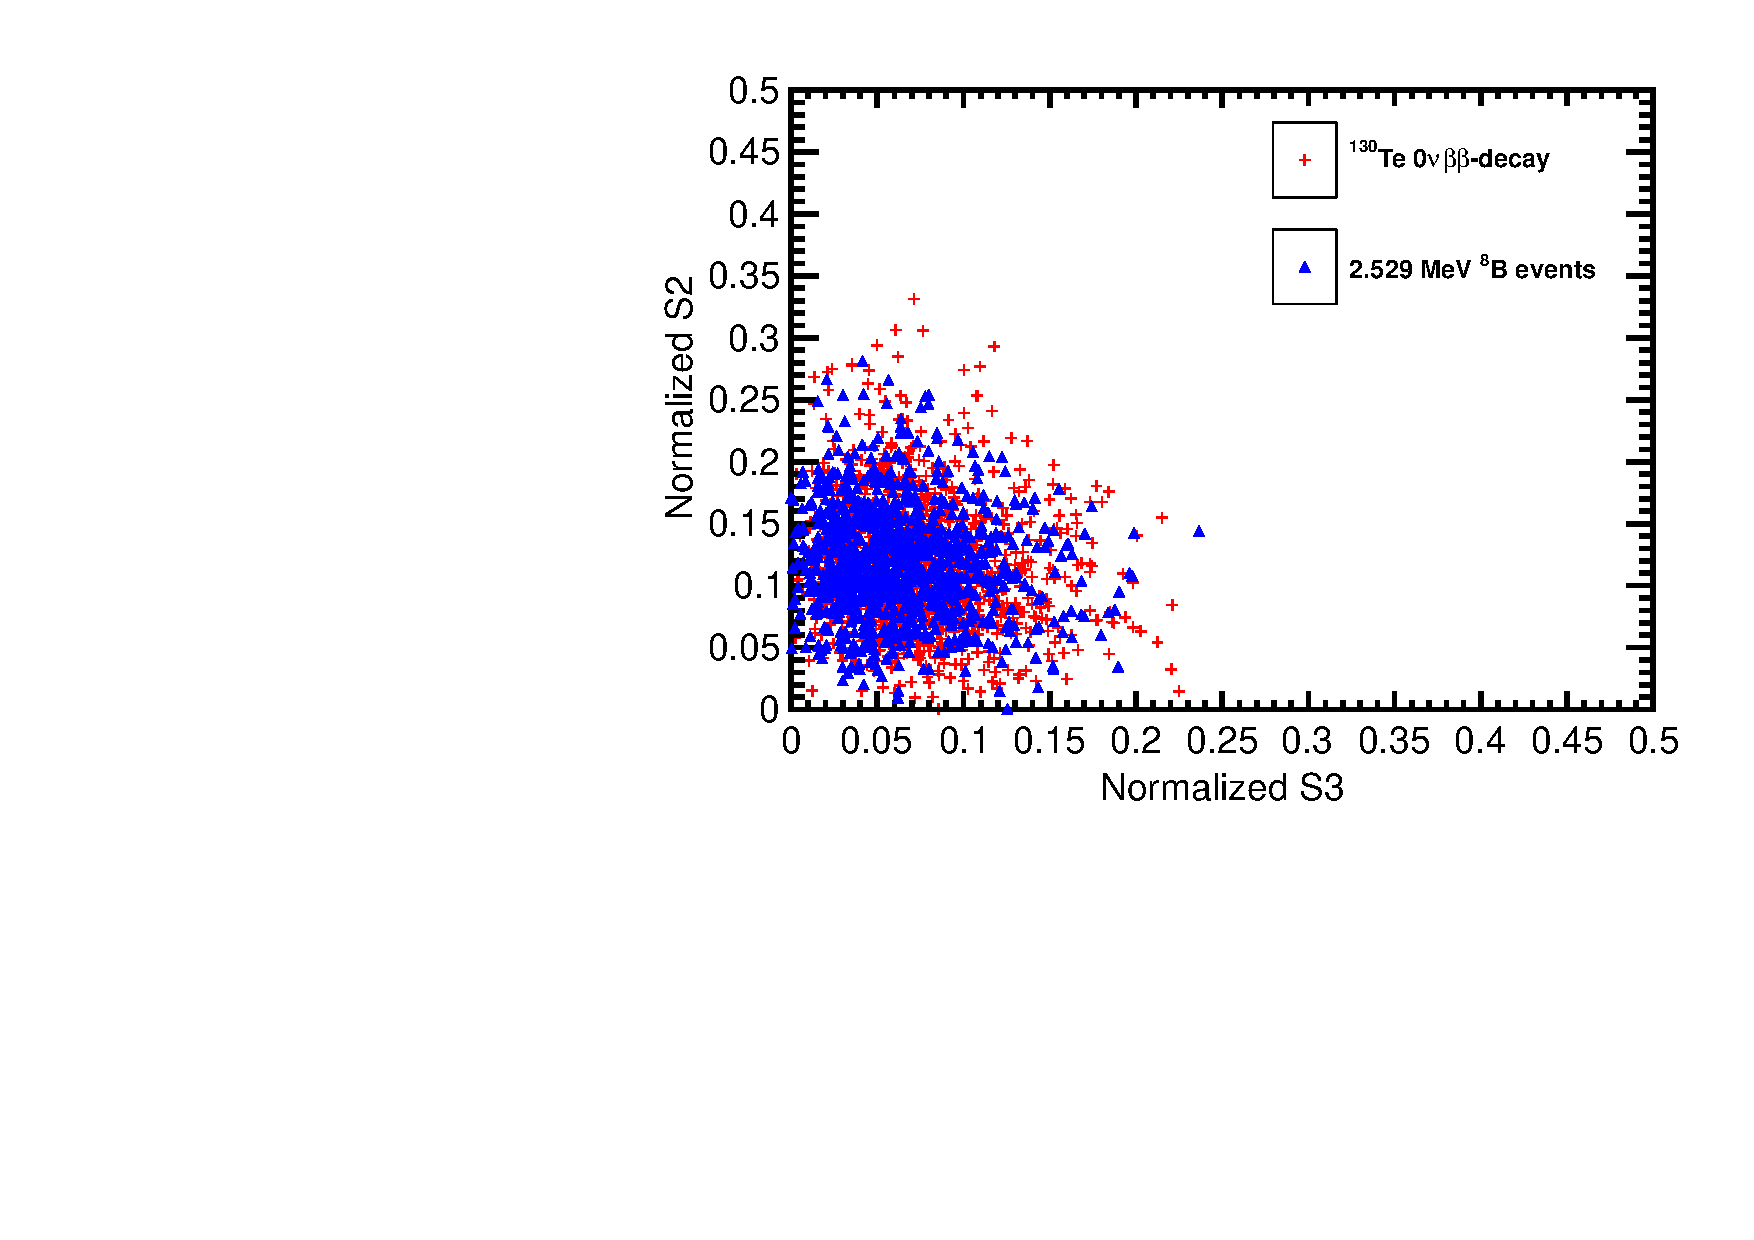
\includegraphics[width=0.49\textwidth]{hS2vsS3_Te130_1el_allLight_VtxSmear0cm_VtxShiftX0cm_33p5ns_center.pdf}
  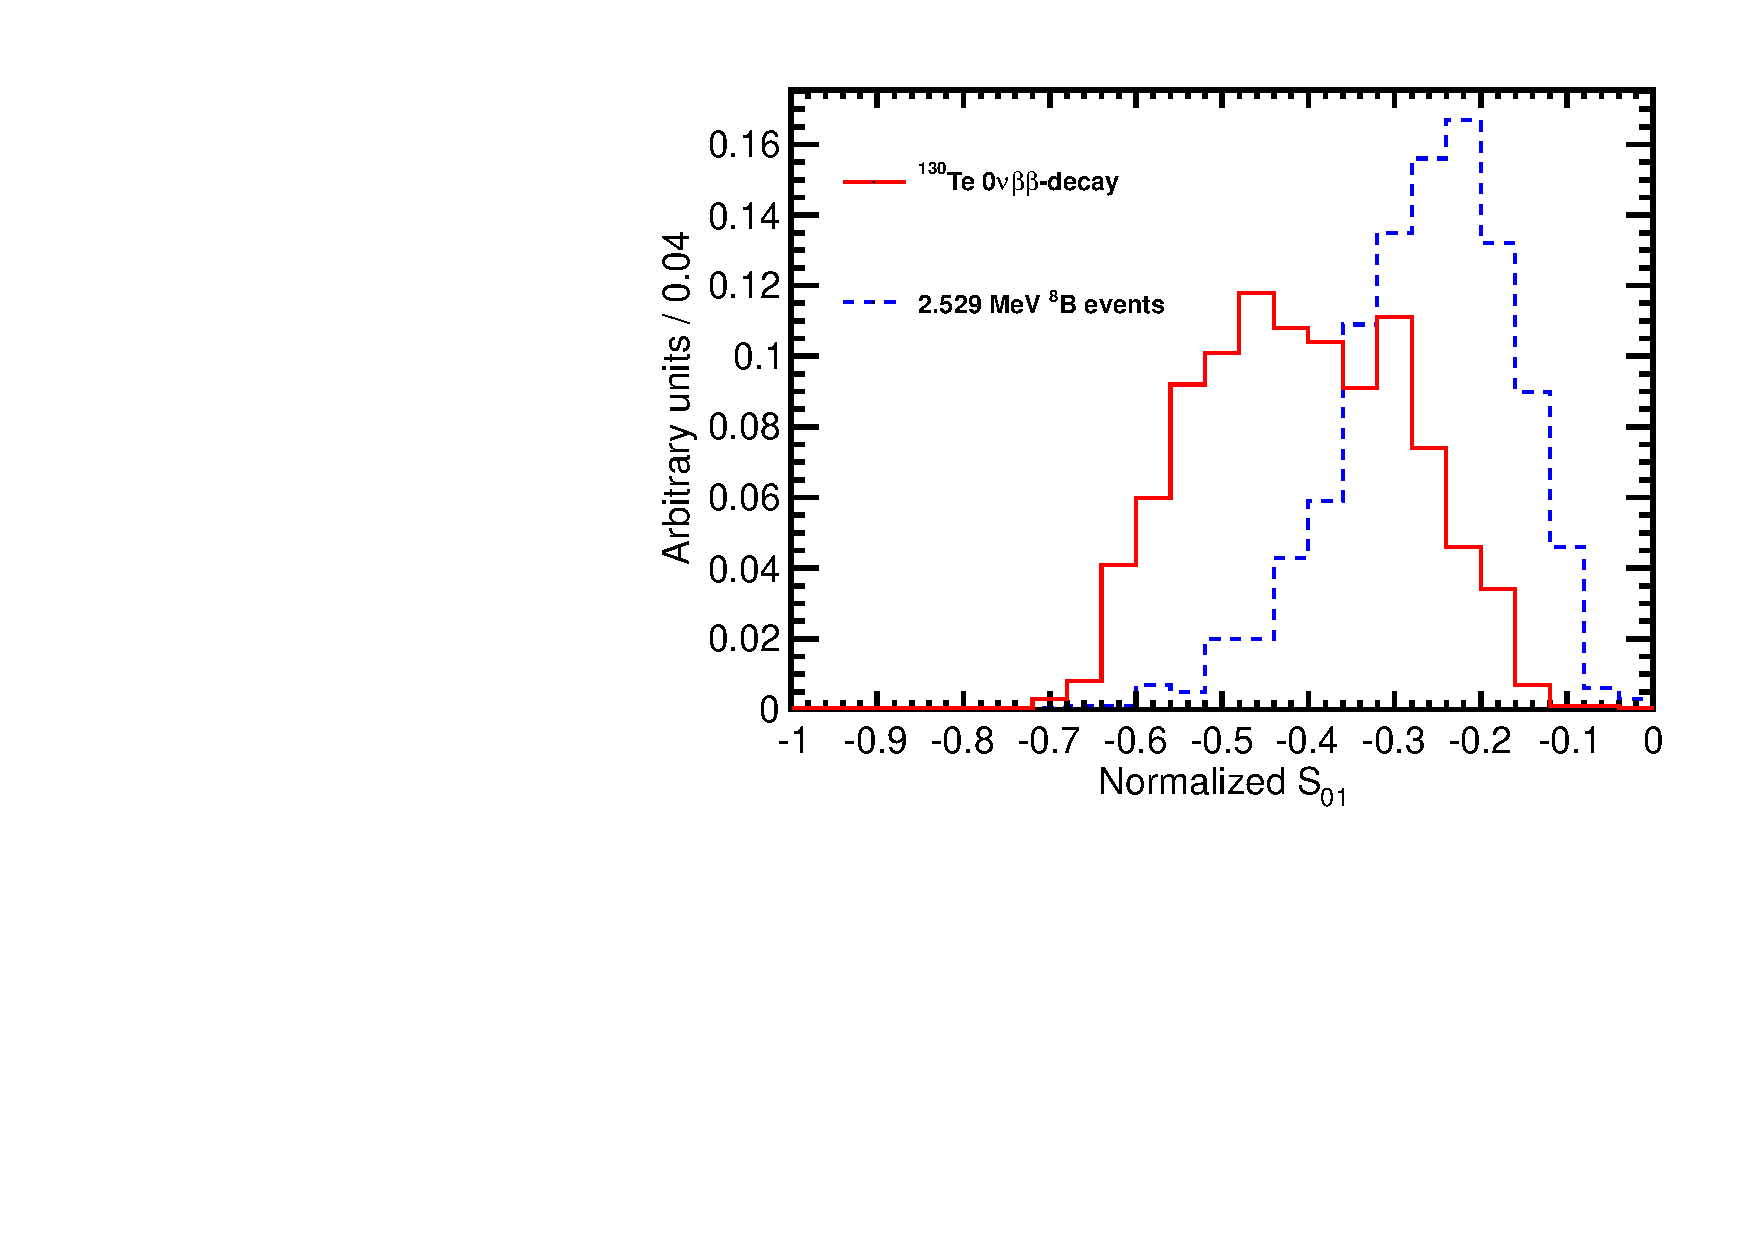
\includegraphics[width=0.49\textwidth]{hS01_allLight_VtxSmear0cm_VtxShiftX0cm_33p5ns_center.pdf}
  \caption{\emph{Left:} Scatter plot of $S_0$ versus $S_1$ for a simulation of 1000 signal (\emph{red crosses}) and background 
    (\emph{blue triangles}) events.
    Central events assuming perfect reconstruction of vertex position. Time cut of 33.5~ns on the PE arrival time is
    applied. The default QE and 100\% photo-coverage is used in the simulation.
    Black dashed line corresponds to a linear fit to define 1-D variable $S_{01}$ (see text for details).
    \emph{Right:} Comparison of the $S_{01}$ distribution between signal (\emph{red solid line}) and background (\emph{blue dashed line}).}
\label{fig:SL_Te_33p5ns_center}
\end{figure*}



\subsection{Experimental challenges}

So far only events at the center of the detector have been considered. Precise vertex reconstruction has been also assumed. 
Here we discuss performance of the spherical harmonics analysis for events that originate thoughout the whole fiducial volume
of the detector and that have limited vertex reconstruction precision.

Selection of early PE sample using absolute time cut of 33.5~ns that has been applied to central events relies on the fact that, 
within the uncertainty on electron track length, all photons travel for the same distance before reaching the surface of the detector. 
PEs with early measured time correspond mostly to Cherenkov photons because of the delay in the scintillation process and longer 
wavelength of the Cherenkov light. 

When the vertex is not at the center, a uniform absolute time cut on the photon arrival time is no longer effective in selecting 
Cherenkov photons. In the case of an off-center vertex, there could be a situation when even significantly delayed scintillation photons 
reach the side of the detector that is closer to the vertex much earlier than Cherenkov photons traveling to the opposite side of the 
detector. Therefore, the time cut has to take into account the total distance traveled by each individual photon.

We found that a differential time cut defined as $\Delta t=t^{phot}_{measured} - t^{phot}_{predicted}<$1~ns selects photons with a 
sufficient fraction being Cherenkov photons. However two factors significantly reduce the Cherenkov/scintillation light 
separation, and therefore, reduce discrimination power of the spherical harmonics analysis, when this relative time cut is applied. 
These factors are chromatic dispersion and vertex resolution. In the following we describe both effects and propose a solution to 
mitigate their influence on the spherical harmonics analysis.

\subsubsection{Chromatic dispersion}
One reduction in the light separation comes from chromatic dispersion. The predicted time, $ t^{phot}_{predicted}=l/v^{phot}$, depends 
on the total distance, $l$, traveled by the photon and the velocity of the photon, $v^{phot}$.  Since the wavelength information is 
not available for a given PE, we must use an average index of refraction of n=1.53 and define the photon velocity as $v^{phot} = c/n$. 
This uncertainty on the photon velocity due to chromatic dispersion reduces the separation between scintillation and Cherenkov light. 

The other reduction in the light separation comes from the uncertainty in the reconstructed vertex position. This uncertainty leads to 
an uncertainty in the photon's total distance traveled and ultimately leads to a reduction in the Cherenkov/scintillation separation.

Since we apply this differential time cut when considering events in the entire fiducial volume, the effectiveness of the spherical 
harmonics analysis in separating of 0{\nbb} decay from $^{8}$B events is reduced. 

We defined fiducial volume as $R<3$~m, where $R$ is the distance between event vertex and the center of the detector.
Figure~\ref{fig:SL_Te_SmearX0cm_momDT1ns_rndVtx_3p0m} demonstrates perfomance of the spherical harmonics analysis for events within this
fiducial volume. Perfect vertex reconstruction is still assumed for events shown in Fig.~\ref{fig:SL_Te_SmearX0cm_momDT1ns_rndVtx_3p0m}. 
Reduced separation between signal and background on Fig.~\ref{fig:SL_Te_SmearX0cm_momDT1ns_rndVtx_3p0m} compared to 
Fig.~\ref{fig:SL_Te_33p5ns_center} is due to the effect of chromatic dispersion which does not allow to achieve as high fraction of 
Cherenkov PEs in the early PE sample as in the case of central events when an absolute time cut is used.


\begin{figure*}[h]
  \centering
  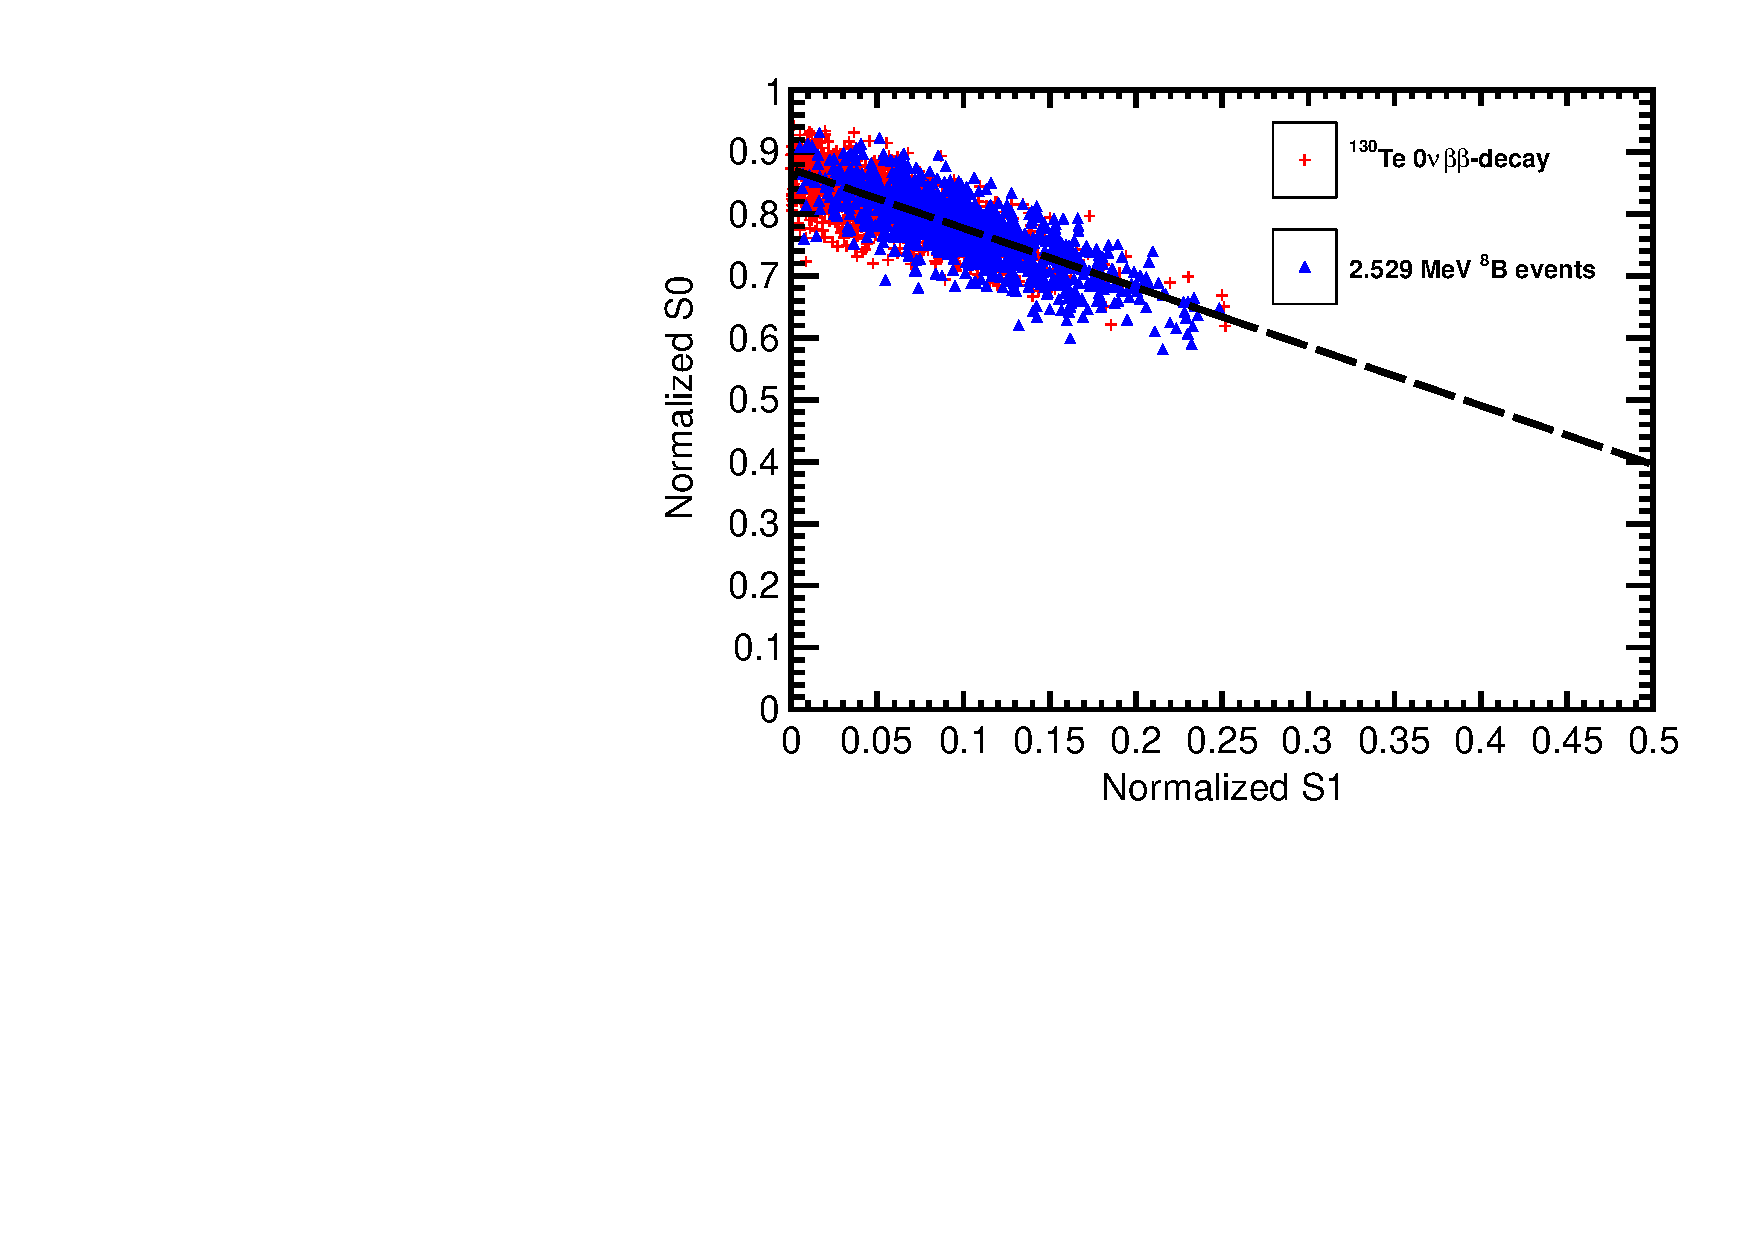
\includegraphics[width=0.49\textwidth]{hS0vsS1_Te130_1el_allLight_VtxSmear0cm_VtxShiftX0cm_momDT1p0ns_rndVtx_3p0mSphere.pdf}
  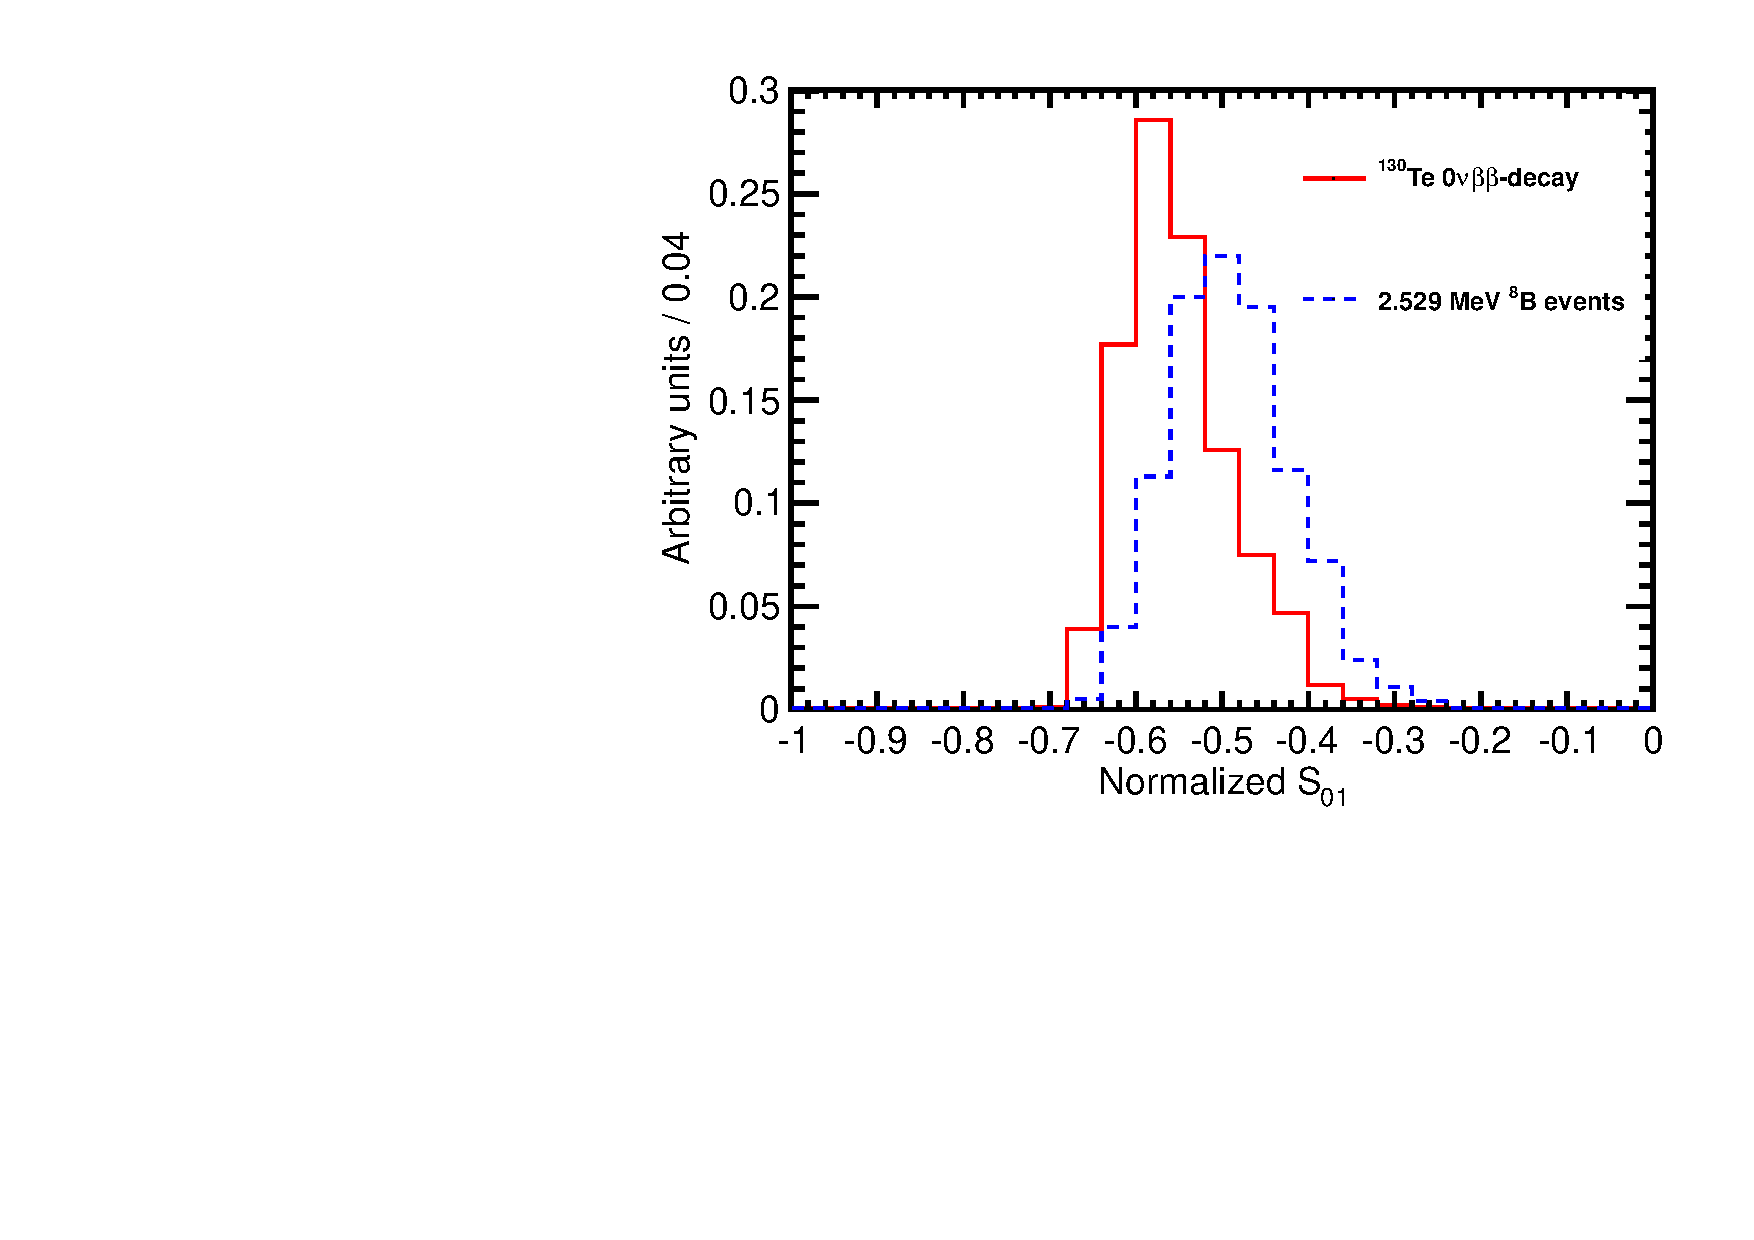
\includegraphics[width=0.49\textwidth]{hS01_allLight_VtxSmear0cm_VtxShiftX0cm_momDT1p0ns_rndVtx_3p0mSphere.pdf}
  \caption{\emph{Left:} Scatter plot of $S_0$ versus $S_1$ for a simulation of 1000 signal (\emph{red crosses}) and background
    (\emph{blue triangles}) events. Event verticies are uniformly distributed within the fiducial volume, $R<3$~m.
    Perfect reconstruction of the vertex position is assumed. Differential cut of 
    $\Delta t=t^{phot}_{measured} - t^{phot}_{predicted}<$1~ns is applied to select early PE sample.
    The default QE and 100\% photo-coverage is used in the simulation.
    Black dashed line corresponds to a linear fit to define 1-D variable $S_{01}$ (see text for details).
    \emph{Right:} Comparison of the $S_{01}$ distribution between signal (\emph{red solid line}) and background (\emph{blue dashed line}).}
  \label{fig:SL_Te_SmearX0cm_momDT1ns_rndVtx_3p0m}
\end{figure*}


\subsubsection{Vertex resolution} 
Imprecise knowledge of the vertex position affects the spherical harmonics analysis in two ways. First, similarly to the effect of chromatic 
dispersion the vertex uncertainty makes differential time cut less efficient in providing sufficient Cherenkov/scintillation light ratio
in the early PE sample. Second, small deviations in vertex reconstruction cause a large effect on the $S_0$ and $S_1$ distributions for the 
single electron event topology.
For the vertices shifted along the direction of the electron track the differential time cut $\Delta t$
reduces the uniformity of the scintillation light distribution. The
$\Delta t$ cut selects more forward emitted photons in the case when
the reconstructed vertex is shifted to the direction opposite to the
electron momentum. This enhances the forward region populated by Cherenkov
photons and causes a more asymmetric photon distribution that moves $S_1$ to higher values\footnote{In general, $S_1$ component of the 
spherical harmonics power spectrum is higher for asymmetric distributions and lower for symmetric distributions (e.g., compare back-to-back
and single electron topologies in Fig.~\ref{fig:ThreeTopologies_Display_5MeV}). Moreover, $S_1=$~0 for a distribution with perfect symmetry 
with respect to the center of the sphere.}.  
The opposite occurs for the case where the reconstructed vertex is shifted in the direction along the electron
momentum. Here, the time cut selects more backward emitted photons and counter balances the forward region populated by Cherenkov
photons leading to a more symmetric photon distribution and smaller values of $S_1$.

Figure~\ref{fig:SL_Te_SmearX3cm_momDT1ns_rndVtx_3p0m} shows the performance of the spherical harmonics analysis for events 
in the fiducial volume, $R<$3~m, after taking into account a 3~cm vertex reconstruction resolution. Finite vertex resolution of 3~cm is
introduced as smearing of the actual simulated vertex position using a Gaussian distribution with sigma of 3~cm along $x$, $y$, and $z$ coordinates.

\begin{figure*}[h]
  \centering
  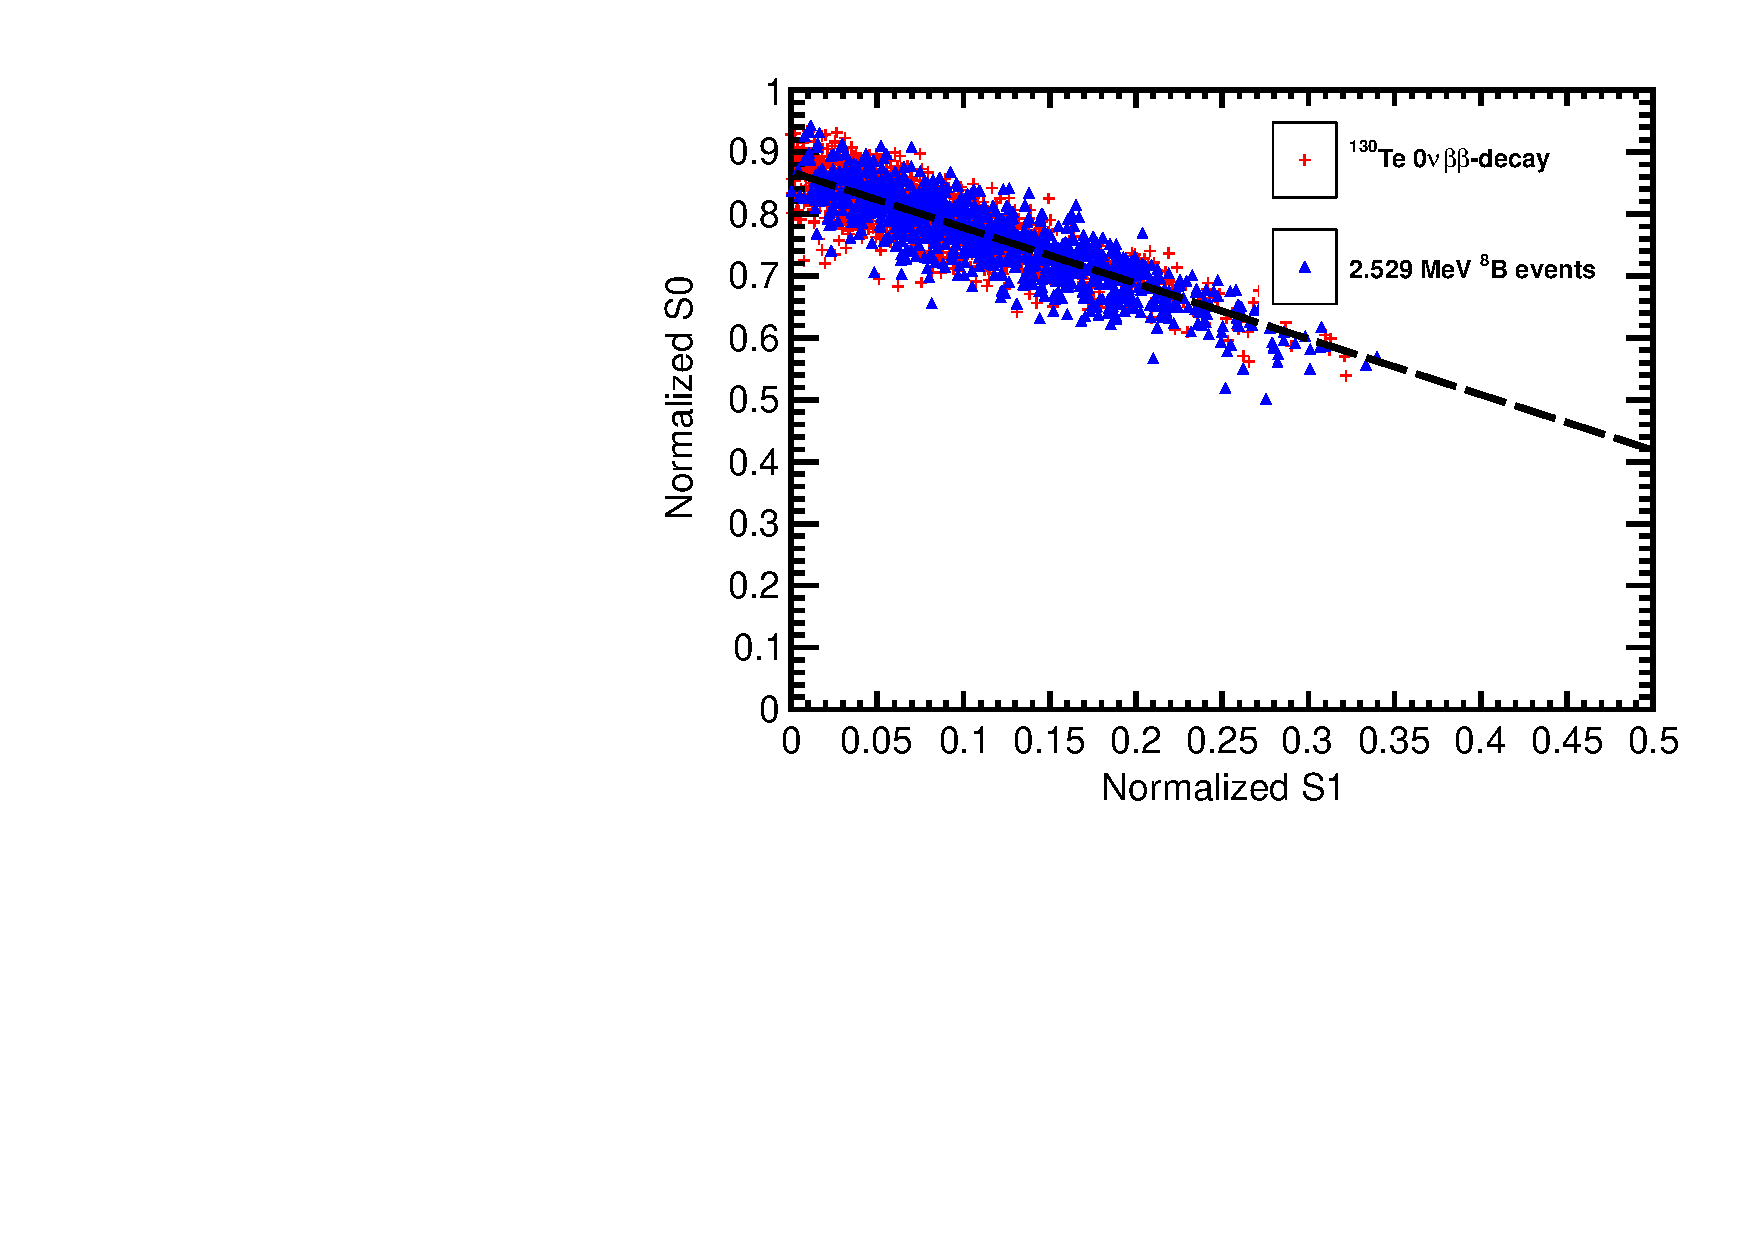
\includegraphics[width=0.49\textwidth]{hS0vsS1_Te130_1el_allLight_VtxSmear3cm_VtxShiftX0cm_momDT1p0ns_rndVtx_3p0mSphere.pdf}
  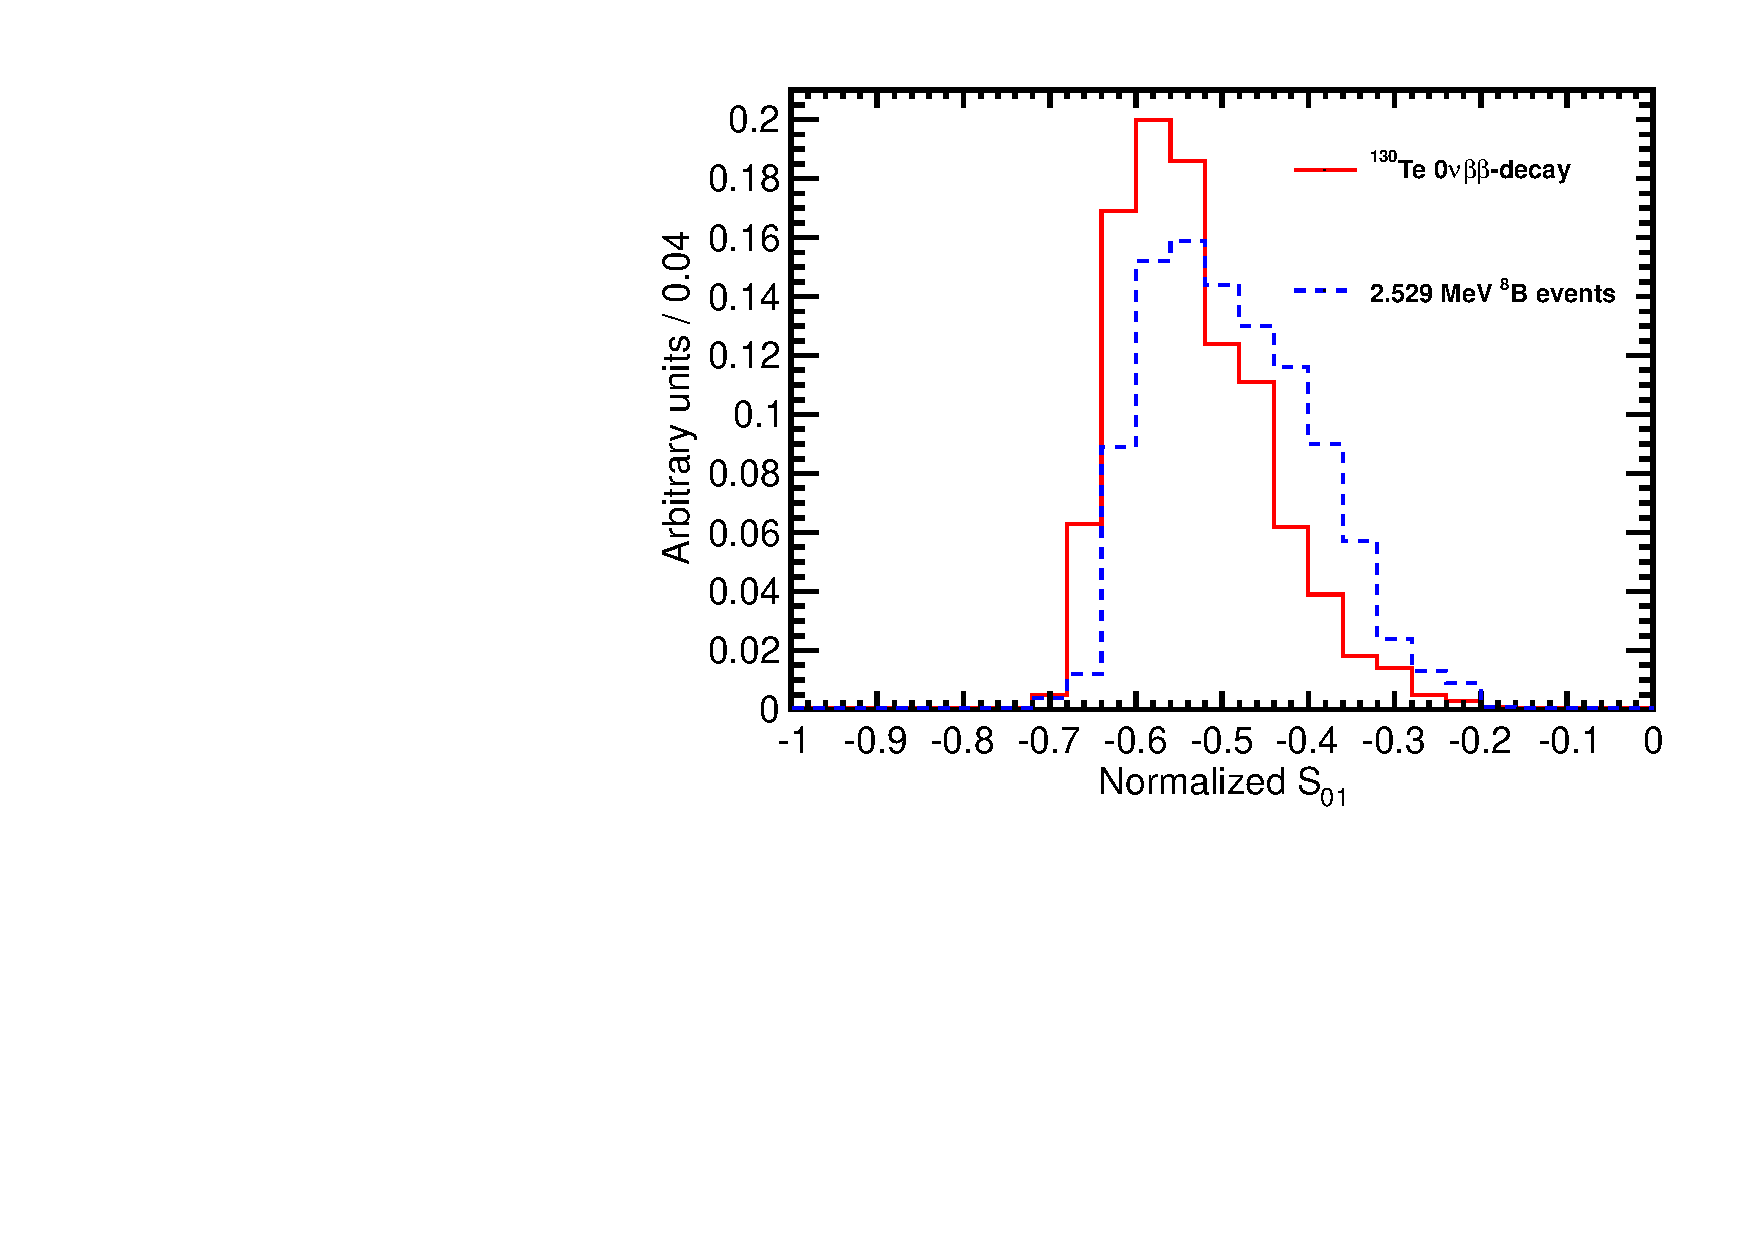
\includegraphics[width=0.49\textwidth]{hS01_allLight_VtxSmear3cm_VtxShiftX0cm_momDT1p0ns_rndVtx_3p0mSphere.pdf}
  \caption{\emph{Left:} Scatter plot of $S_0$ versus $S_1$ for a simulation of 1000 signal (\emph{red crosses}) and background
    (\emph{blue triangles}) events. Event verticies are uniformly distributed within the fiducial volume, $R<3$~m.
    Vetrex is smeared with 3~cm resolution. Differential cut of
    $\Delta t=t^{phot}_{measured} - t^{phot}_{predicted}<$1~ns is applied to select early PE sample.
    The default QE and 100\% photo-coverage is used in the simulation.
    Black dashed line corresponds to a linear fit to define 1-D variable $S_{01}$ (see text for details).
    \emph{Right:} Comparison of the $S_{01}$ distribution between signal (\emph{red solid line}) and background (\emph{blue dashed line}).}
\label{fig:SL_Te_SmearX3cm_momDT1ns_rndVtx_3p0m}
\end{figure*}

As can be seen in Fig.~\ref{fig:SL_Te_SmearX3cm_momDT1ns_rndVtx_3p0m}, the vertex resolution significantly reduces the discrimination power 
of the spherical harmonics analysis for our default detector model.

%{\bf Solution to this problem would be a better selection criteria of
%  early light. It has to preserve high admixture of the Cherenkov
%  photons, but needs to select scintillation photons in a more uniform
%  manner. Working on it, but may not be simple so I don't want to
%  include it in this paper.}


\subsubsection{Requirements for the next generation liquid scintillator detectors}
To take full advantage of topology reconstruction capabilities in the next generation liquid scintillator detectors optical properties of the 
scintillator has to be tuned to allow for better Cherenkov/scintillation light separation.

The effects due to chromatic dispersion can be addressed by using liquid scintillators with a more narrow emission spectrum. For example,
such as described in Ref.~\cite{LS_narrow_emission}.

Strong dependence on the vertex resolution can be addressed by choosing a liquid scintillator mixture with a more delayed emission 
of scintillation light with respect to Cherenkov light. With a larger delay in scintillation light, a high fraction of Cherenkov light 
in the early PE sample can be maintained even if photon track length is mis-reconstructed due to imprecise reconstruction of the vertex 
position. In addition, if the fraction of scintillation light is small compared to Cherenkov light, the distortions in the uniformity of 
the scintillation PE due to shifted reconstructed vertex position would not significantly affect spherical harmonics power spectrum.


\textbf{Text below hasn't been revised yet. 5ns rise time will be implemented instead of unphysical 0.5~ns delay.}

Figure~\ref{fig:SL_Te_momDT1ns_sci0p5ns_rndVtx_3p0m} shows
spherical harmonics analysis for the simulation where the
scintillation component is delayed by an additional 0.5ns compared to our default simulation. Events are simulated uniformly within the fiducial volume of the detector. Vertex resolution of 3~cm is assumed. Noticeable separation between \nbb and \B~events is achieved.

The discrimination power of the spherical harmonics analysis improves with vertex resolution and more delay in the emission of the scintillation light. Moreover the dependence on vertex reconstruction reduces with delay in the scintillation light. 

\begin{figure*}[h]
  \centering
  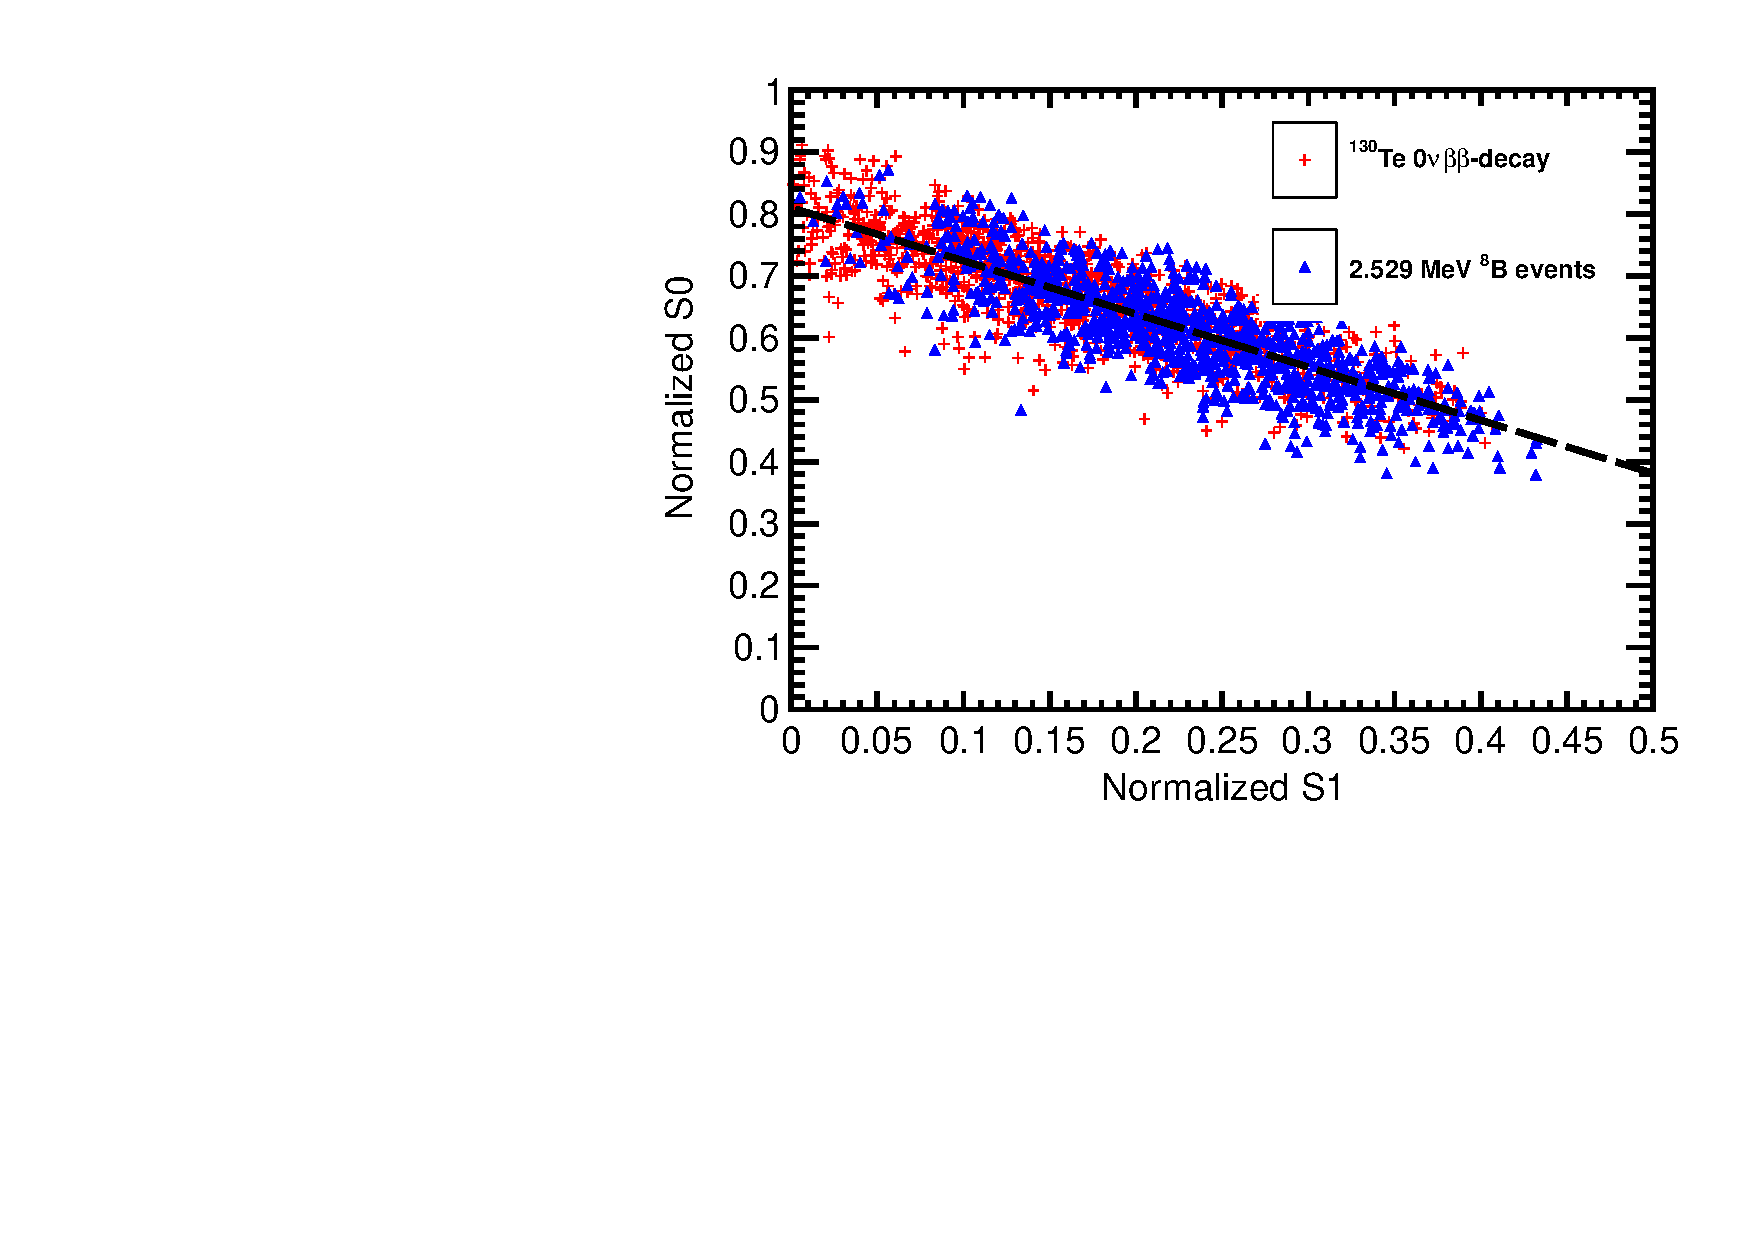
\includegraphics[width=0.49\textwidth]{hS0vsS1_Te130_1el_allLight_VtxSmear3cm_VtxShiftX0cm_momDT1p0ns_sci0p5ns_rndVtx_3p0mSphere.pdf}
  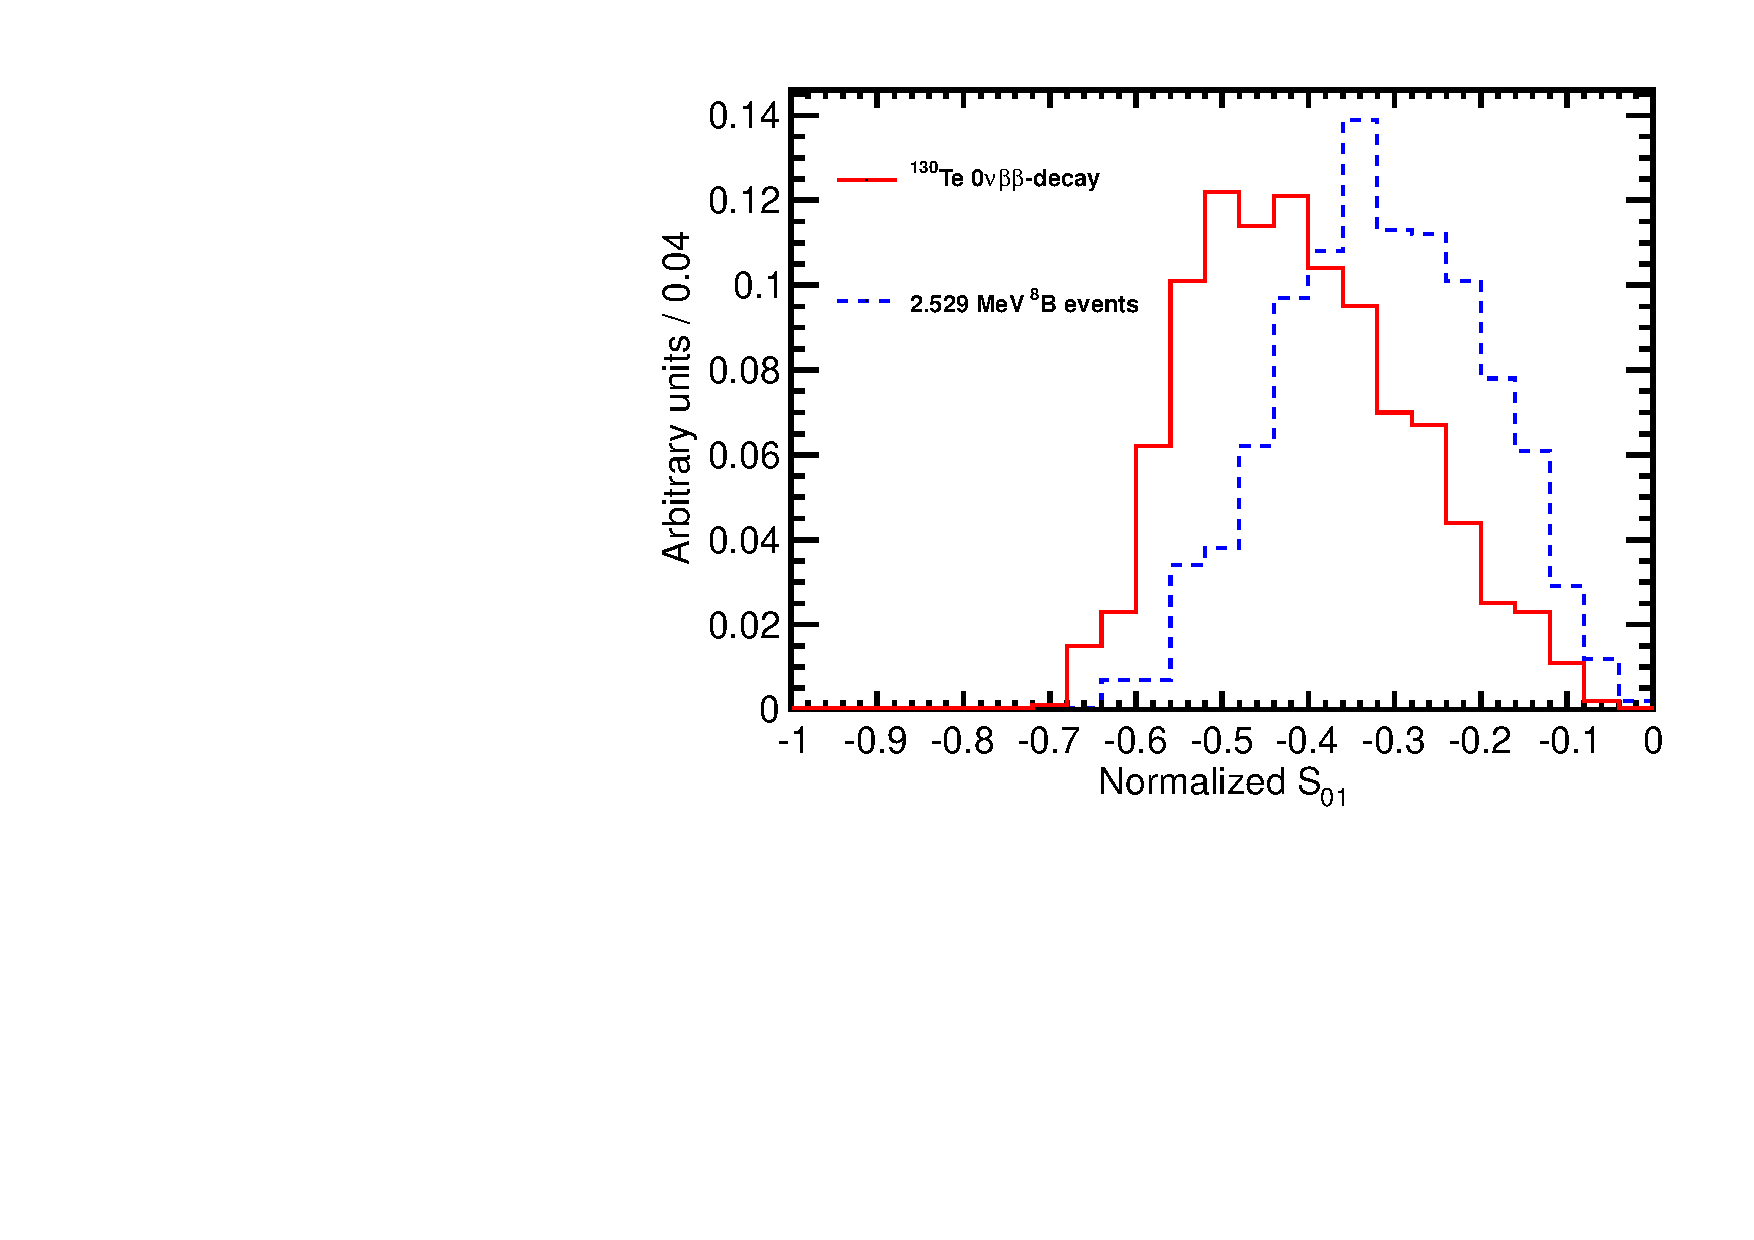
\includegraphics[width=0.49\textwidth]{hS01_allLight_VtxSmear3cm_VtxShiftX0cm_momDT1p0ns_sci0p5ns_rndVtx_3p0mSphere.pdf}
  \caption{Spherical harmonics comparison between $^{130}$Te 0{\nbb}
    decay signal ($Q=2.529$~MeV) (\emph{red}) and $^{8}$B solar
    neutrinos background (\emph{blue}) for 1000 simulated
    events. Verticies are uniformly distributed within the fiducial
    volume, $R<3$~m. $^8$Be events are implemented as 2.529~MeV
    electrons with the initial momentum direction uniformly
    distributed within 4$\pi$ solid angle. Vetrex is smeared with 3~cm
    resolution. {\bf Scintillation light is delayed by additional
      0.5~ns.} \emph{Left:} $S_0$ versus $S_1$ scatter plot. Black dotted
    line is a linear fit of these 2D histograms. Variable $S_{01}$ is
    defined as a projection of 2D distribution onto this linear
    fit. \emph{Right:} $S_{01}$}
\label{fig:SL_Te_SmearX3cm_momDT1ns_sci0p5ns_rndVtx_3p0m}
\end{figure*}



\clearpage %These are only needed to force correct placement of the
           %figures while there is no text

\section{Conclusions}
\label{sec:conclusions}
We consider the use of large-area photodetectors with good time and
space resolution in kiloton scale liquid scintillator detectors to
suppress background coming from $^{8}$B solar neutrino
interactions. Using a default model detector with parameters derived
from present practice, we show that a sample of detected photons
enriched in Cherenkov light by a cut on time-of-arrival contains
directional information that can be used to separate 0{\nbb}~ decay from
$^{8}$B solar neutrino interactions. The separation is based on a
spherical harmonics analysis of the event topologies of the
two electrons in signal events and the single electron in the
background. The performance of the technique is constrained by
chromatic dispersion, vertex reconstruction, and the time profile of
the emission of scintillation light. The development of a scintillator
with a rise time constant of at least 5~ns would allow a
Cherenkov-scintillation light separation with a background rejection
factor for \B~ solar neutrinos of xx and an efficiency for 0\nbb~ signal
of xx\%.



\clearpage %These are only needed to force correct placement of the
           %figures while there is no text

\section*{Acknowledgements}
The activities at the University of Chicago  were supported by the
Department of Energy under DE-SC-0008172, the
National Science Foundation under grant PHY-1066014, and the Driskill
Foundation, and at MIT by  the
National Science Foundation under grant 1554875.

We thank G. Orebi Gann of UC for a discussion on expected backgrounds
at the SNO+ experiment, and J.  Kotilla for discussions on electron
angular correlations in 0\nbb-decay and for providing data with phase
factors for generating 0\nbb- and 2\nbb-decay events.  We are grateful
to C. Aberle for initial development of the Geant-4
detector model used in this paper and for contributions to the
development of the Cherenkov/scintillation light separation technique, and
to M.  Wetstein for help with vertex reconstruction algorithms and
productive discussions on Cherenkov/scintillation light separation. We
thank E. Spieglan for productive discussions on spherical harmonics
analysis and E. Angelico for estimating the effects of photo-detector
position and time resolution on the vertex reconstruction and
verifying the effects of chromatic dispersion.  We thank J. Flusser
for helpful discussions on image processing using moment
invariants. Last but not least we thank M. Yeh for discussions of the
timing properties of liquid scintillators.


\bibliography{bibliography.bib}

\appendix
% The following line is a hack for elsevier to get the appendix and
% the table of contents to play well together.
\renewcommand*{\thesection}{\Alph{section}}
\section{Timing of photons coming from $^{10}$C background}

Typical energy deposition by $^{10}$C events is shown in
Fig.~\ref{fig:Edep_C10}. Assuming $\sim$15\% energy resolution, events in 
the energy range of 2.1-2.9~MeV would contribute to the backgroung count in 
the ROI.


\begin{figure}[h]
  \centering
  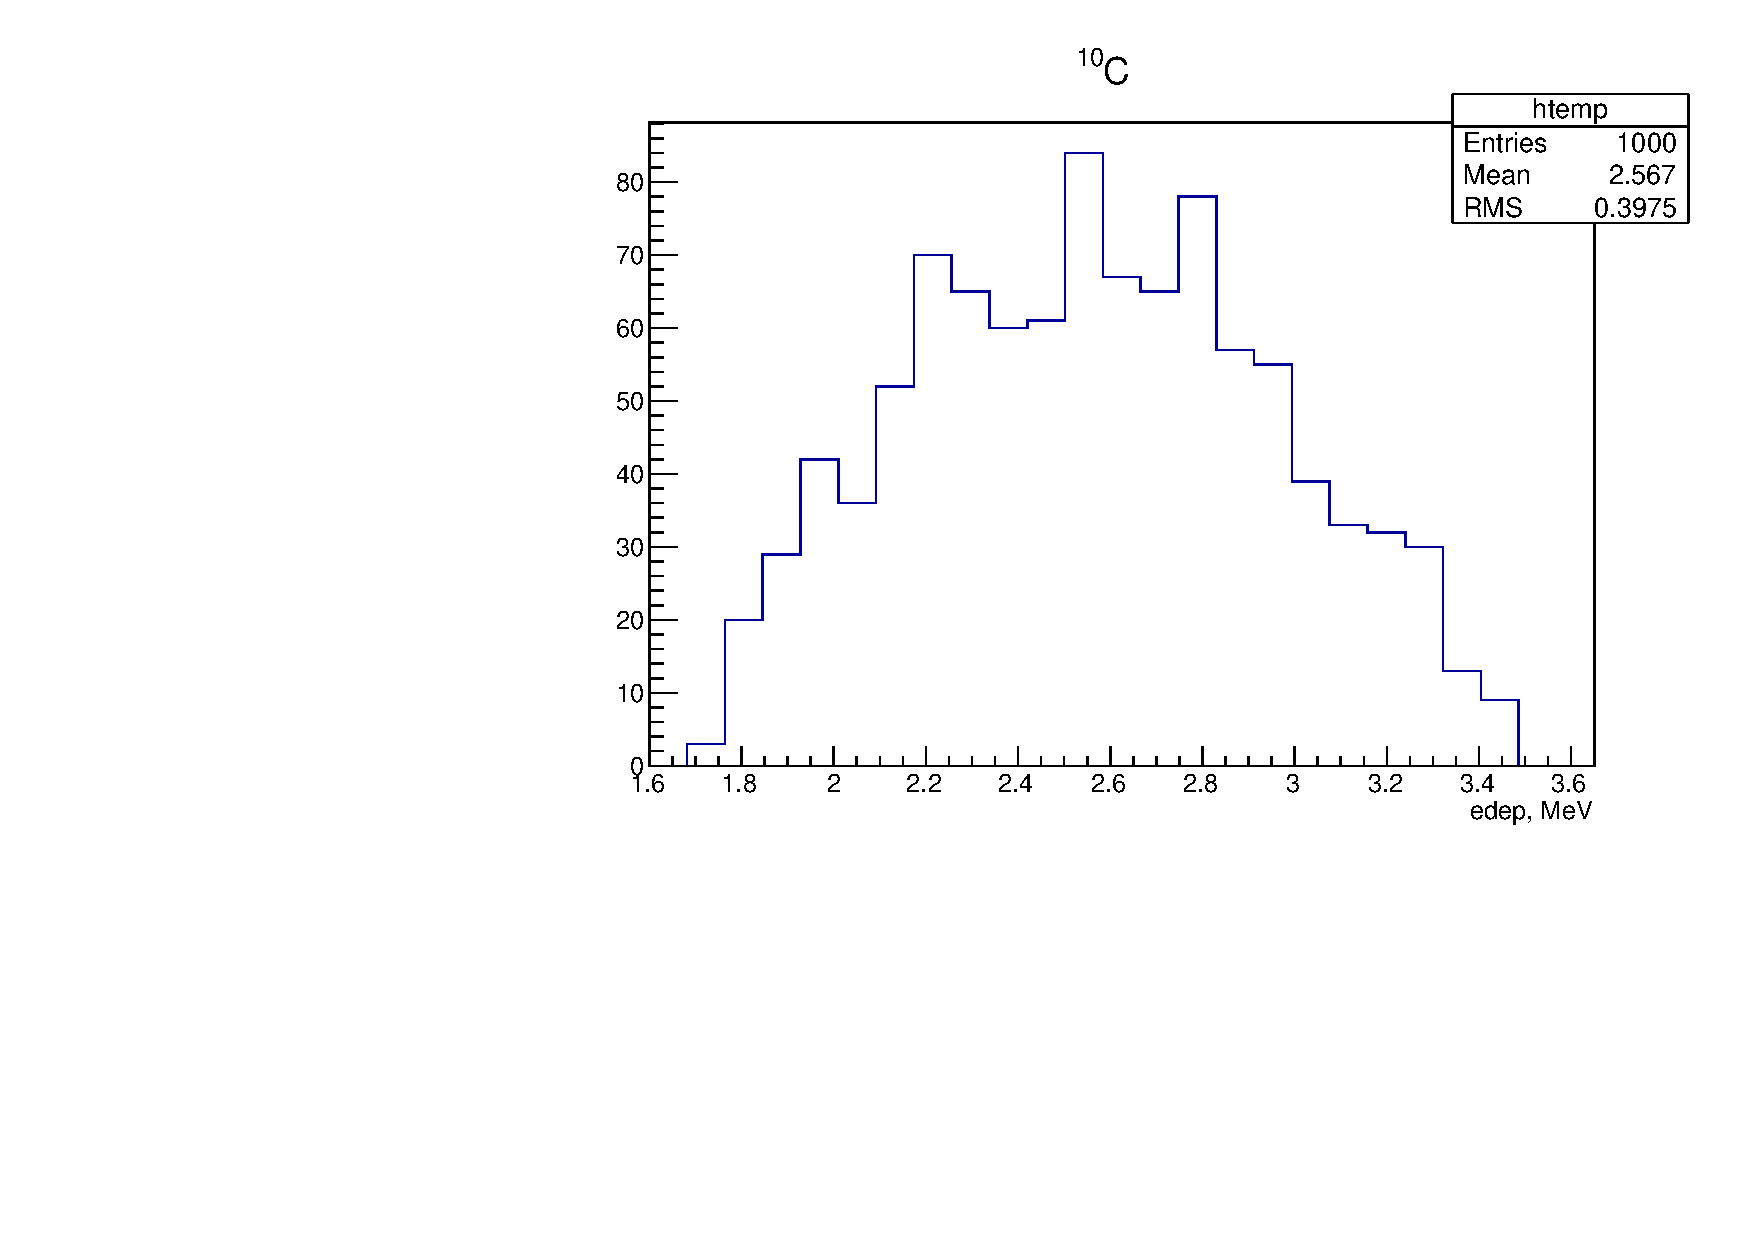
\includegraphics[width=0.95\textwidth]{hEdep_C10.pdf}
  \caption{Energy deposition in $^{10}$C events.}
  \label{fig:Edep_C10}
\end{figure}

Since 98\% of $^{10}$C decays through an excited state of $^{10}$B(718), 
which has a half-life time of $\sim$1~ns, the majority of $^{10}$C events have 
a prompt positron accompanied by a delayed 0.718~MeV gamma. The positron energy
has to be 0.79~MeV for an event to have energy deposition equal to Q-value of
$\Te$ $\vbb$-decay.

The positron from $\Cten$ on average travels 4~mm before it stops and anihilates
producing two 0.511~MeV gammas. Those gammas then interact in the scintillator via 
Compton scattering and photo-electric effect along while they loose their energy
over $\sim X_0$ distance. Therefore light emmited in $\Cten$ events originates from
several clusters that are spread over $\sim X_0$. Significant fraction of the 
early PE would be due to primary positron cluster. Because the positron has smaller 
kinetic energy than kinetic energy of electrons from $\vbb$-decay the amount of early 
PE is smaller for $\Cten$ events. Delayed 0.718~MeV gamma in some of $\Cten$ events 
also result in a delay in the photon arrival time with respect to $\vbb$-decay events.

Figure~\ref{fig:Arrival_time_C10_overlaid} compares PE arrival times between 
$\vbb$-decay and $\Cten$ events. Prompt $\Cten$ is a simplified simulation where 
a positron is simultaneously produced with 0.718~MeV gamma. The difference between
prompt $\Cten$ and $\vbb$-decay is caused by presence of a positron and this 
difference is typical event by even basis. An additional difference due to delayed
gamma shown in Fig.~\ref{fig:Arrival_time_C10_overlaid} is an average over 1000 events.

\begin{figure}[h]
  \centering
  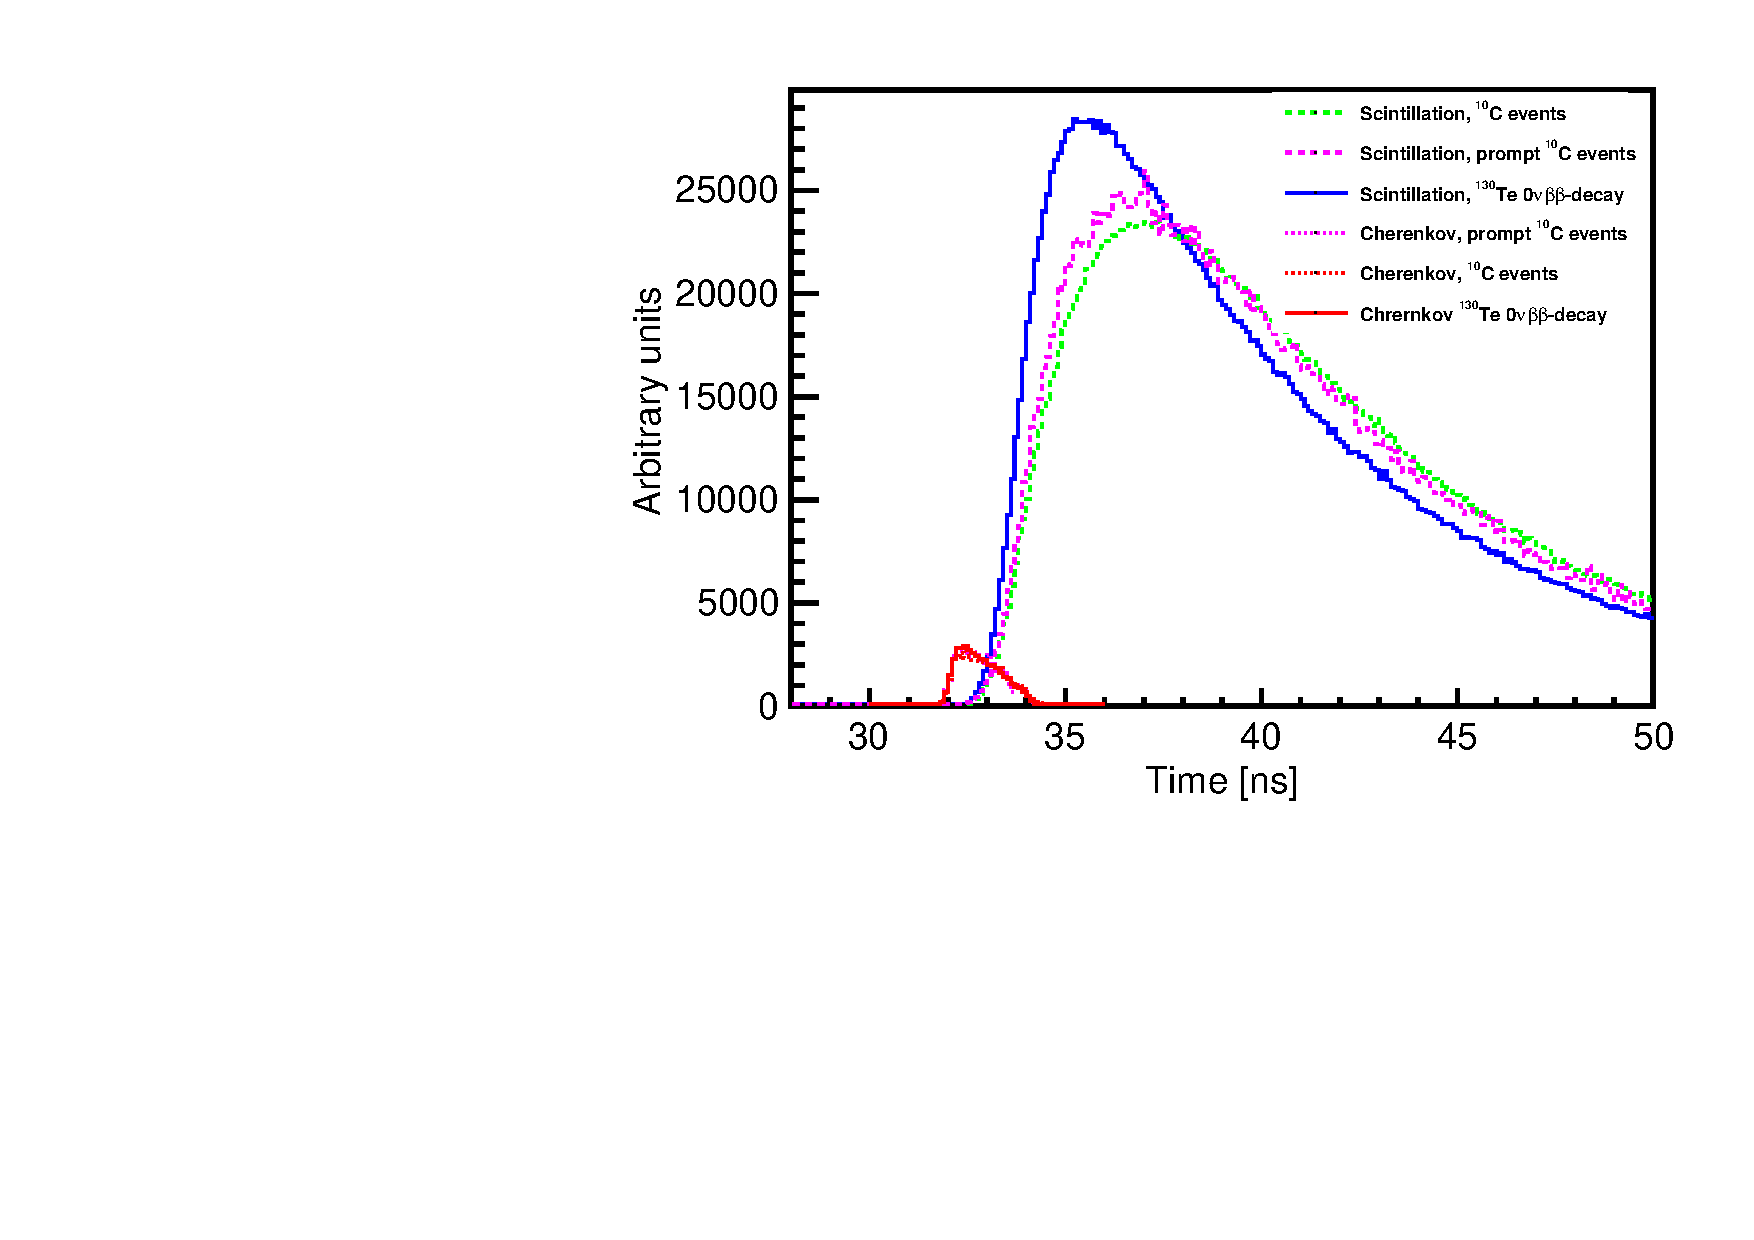
\includegraphics[width=0.95\textwidth]{hT_Te130vsC10_overlaid_v2.pdf}
  \caption{Photo-electron (PE) arrival times after application of the
    photo-detector transit time spread (TTS) of 100~ps for the
    simulation of 1000 0{\nbb} decay events of $^{130}$Te (\emph{solid
      lines}) and $^{10}$C (\emph{dotted lines}) events at the center
    of the detector. Cherenkov and scintillation components are are normalized for 
    for shape comparison.}
\label{fig:Arrival_time_C10_overlaid}
\end{figure}

To distinguish between $\vbb$-decay and $\Cten$ we count total number of PEs in the 
early light sample. For central events where we assume perfect knowledge of the 
primary vertex location the early light sample is defined as t$<$33.5~ns. For a more 
realistic scenario where the vertex is uniformly distributed within the fiducial volume
the early light sample is defined as $\Delta t=t^{phot}_{measured} - 
t^{phot}_{predicted}<$1~ns.


Number of Cherenkov and scintillation PEs in early light samples for $\vbb$-decay and 
$\Cten$ central events is shown in Fig.~\ref{fig:NPhotDist_C10}. Here a perfect 
reconstrution of the primary vertex is assumed. Figure~\ref{fig:NPhot_compare_central} shows
separation between $\vbb$-decay and $\Cten$ events by counting total number of PEs. 

\begin{figure*}[ht]
  \centering
  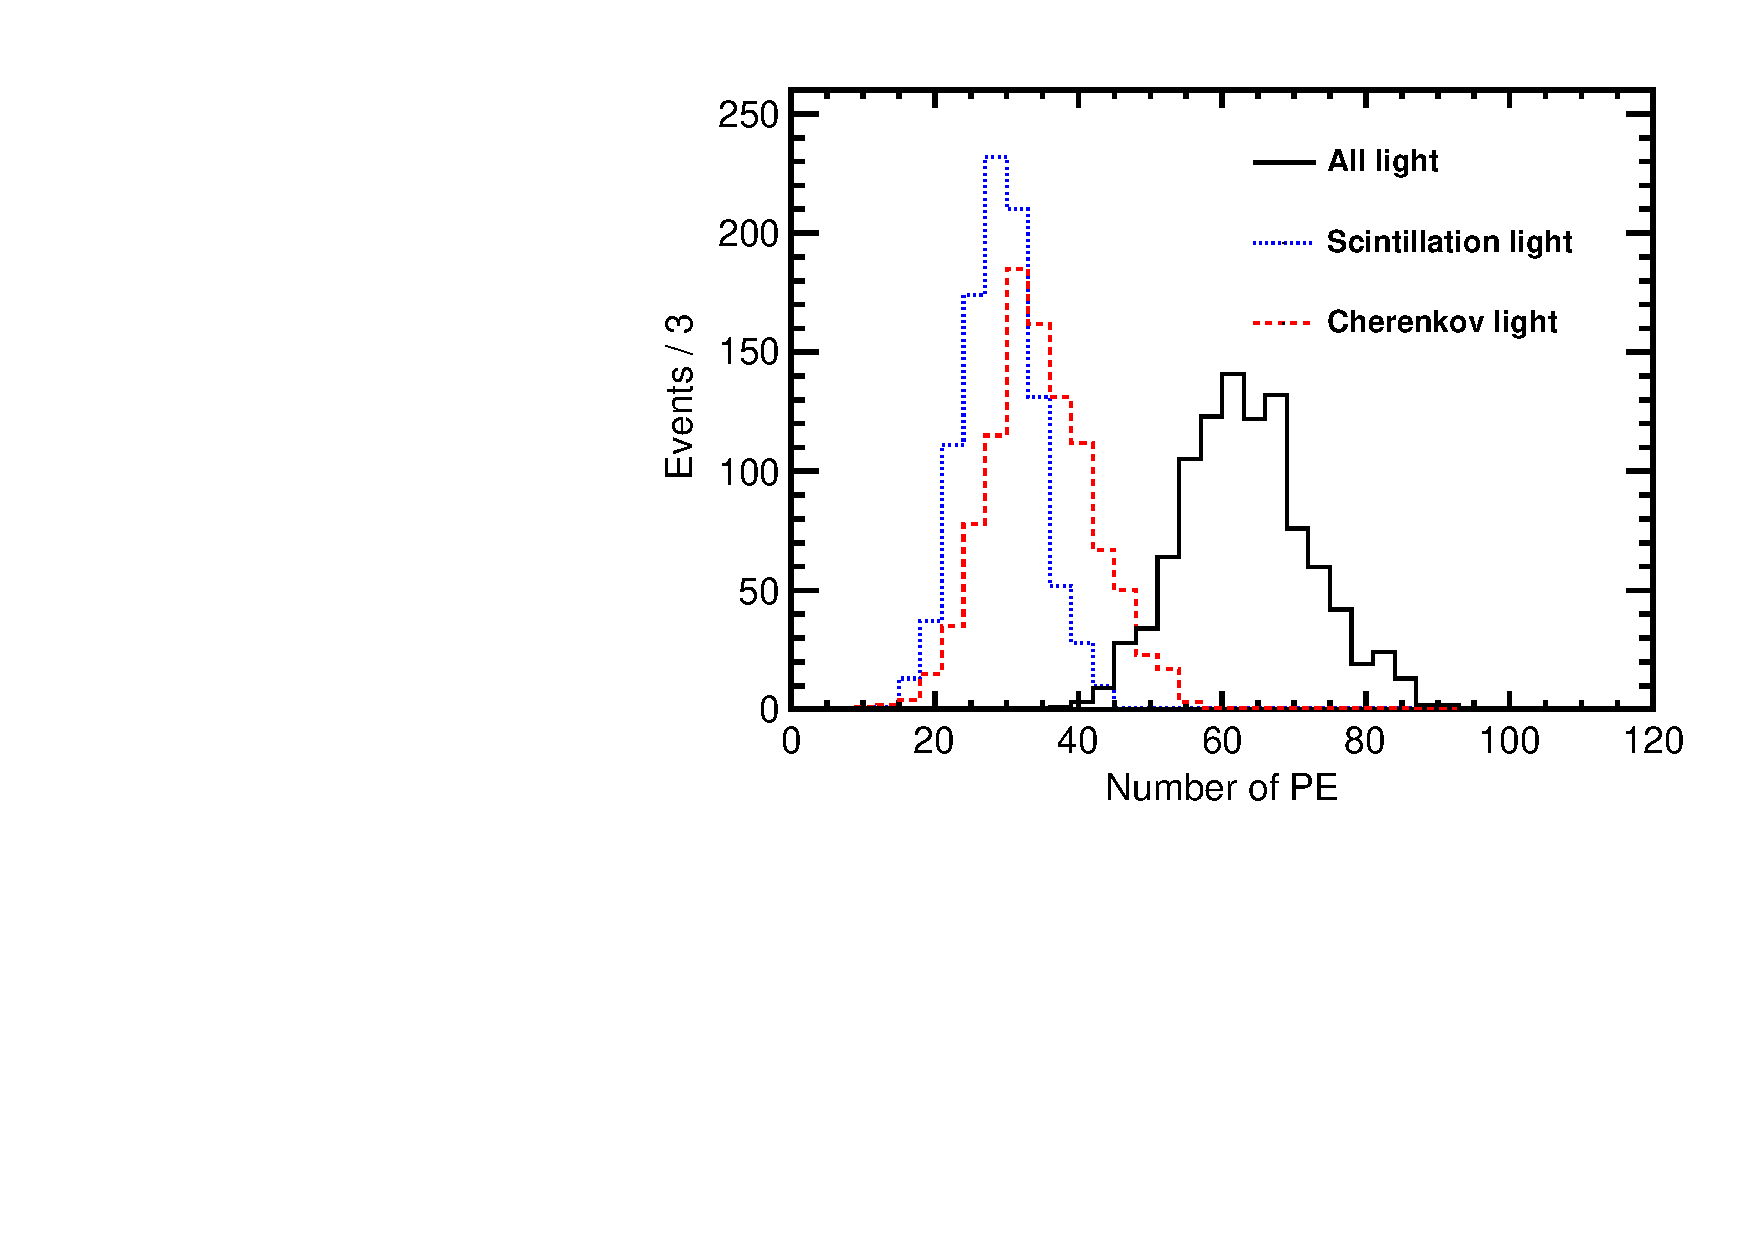
\includegraphics[width=0.45\textwidth]{hMomNPhot_Te130.pdf}
  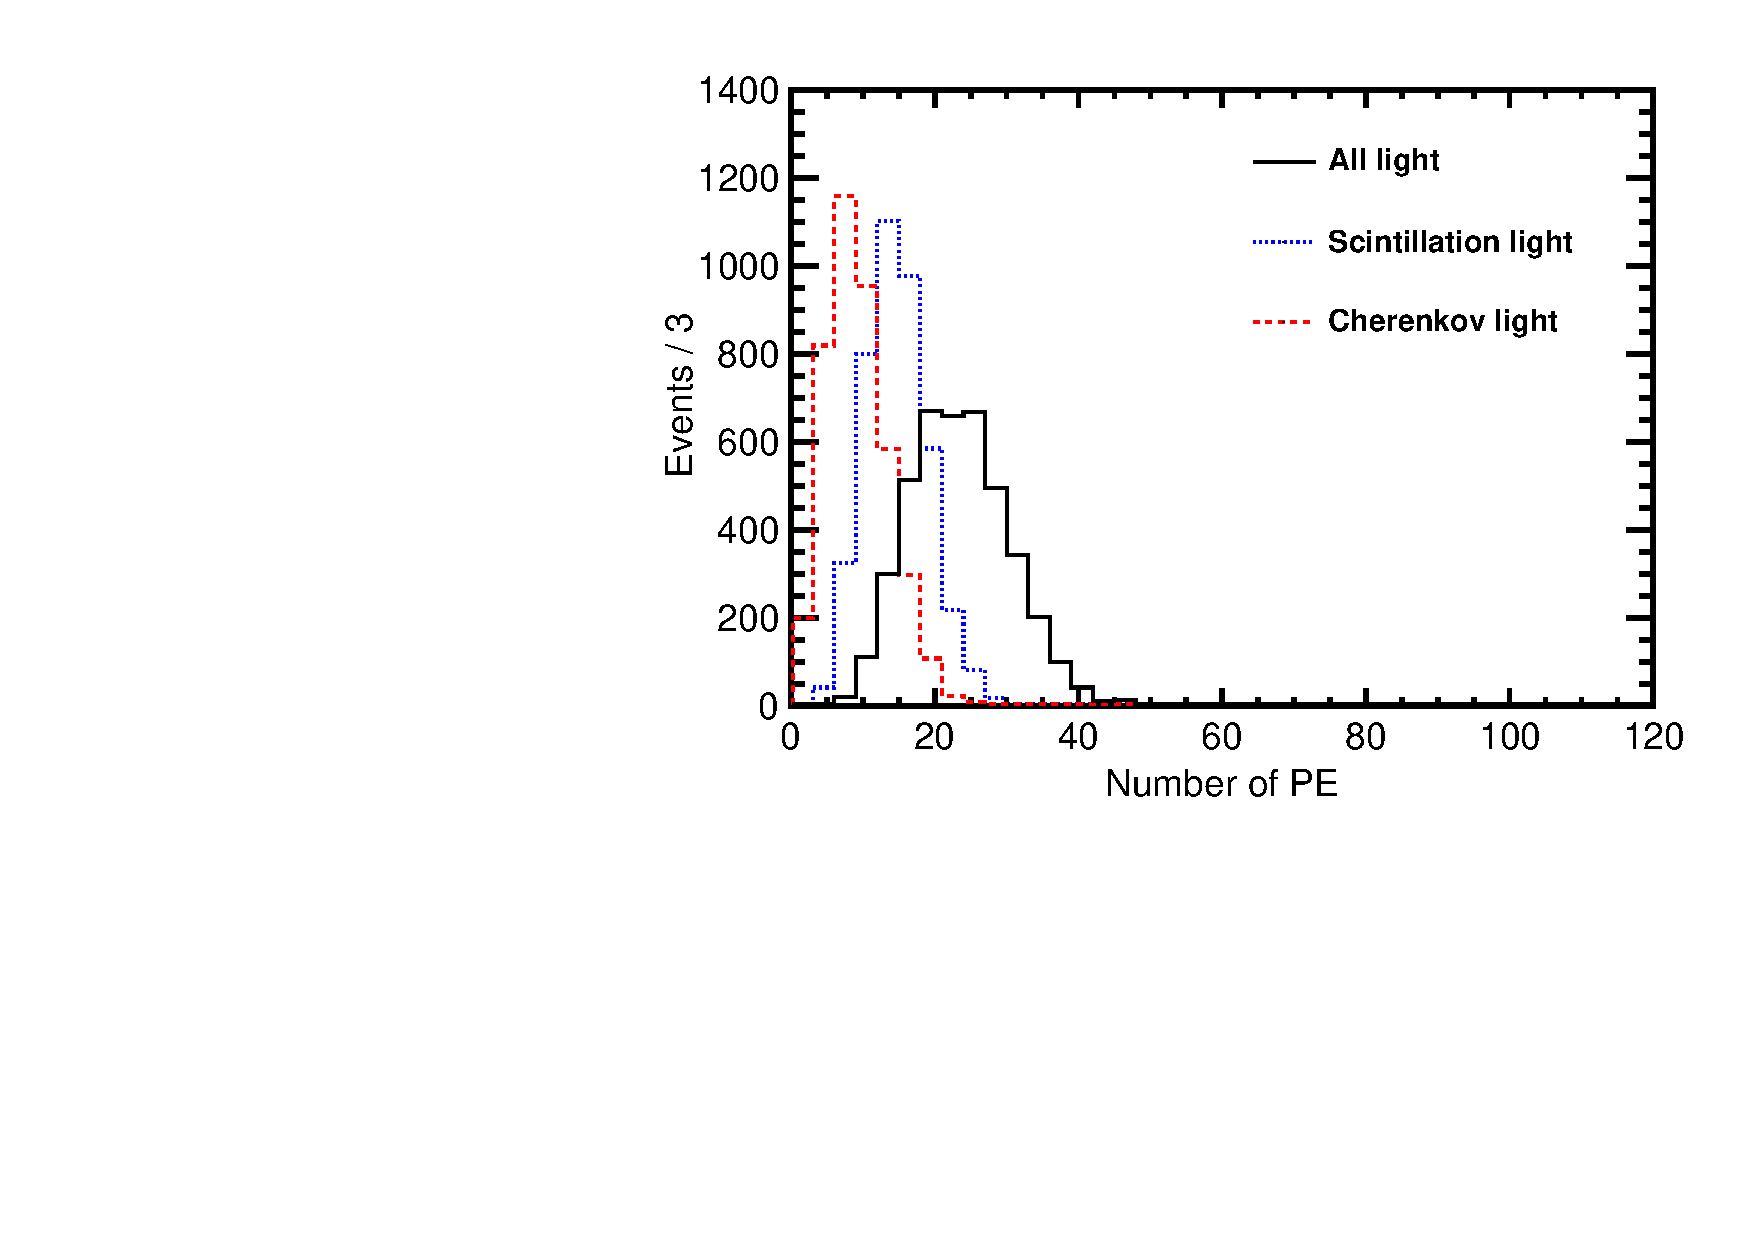
\includegraphics[width=0.45\textwidth]{hMomNPhot_C10.pdf}
  \caption{Early photons. Number of Cherenkov (\emph{dashed red line}), 
    scintillation
    (\emph{dotted blue line}), and total (\emph{solid black line}) PEs
    for the simulation of 1000 $^{130}$Te 0{\nbb} decay (left panel)
    and of 648 $^{10}$C (\emph{right panel}) events (1000 $^{10}$C events was 
    generated, but selected only those that has total energy deposition in the 
    detector in the range between 2.1 and 2.9~MeV).}
\label{fig:NPhotDist_C10}
\end{figure*}



\begin{figure*}[ht]
  \centering
  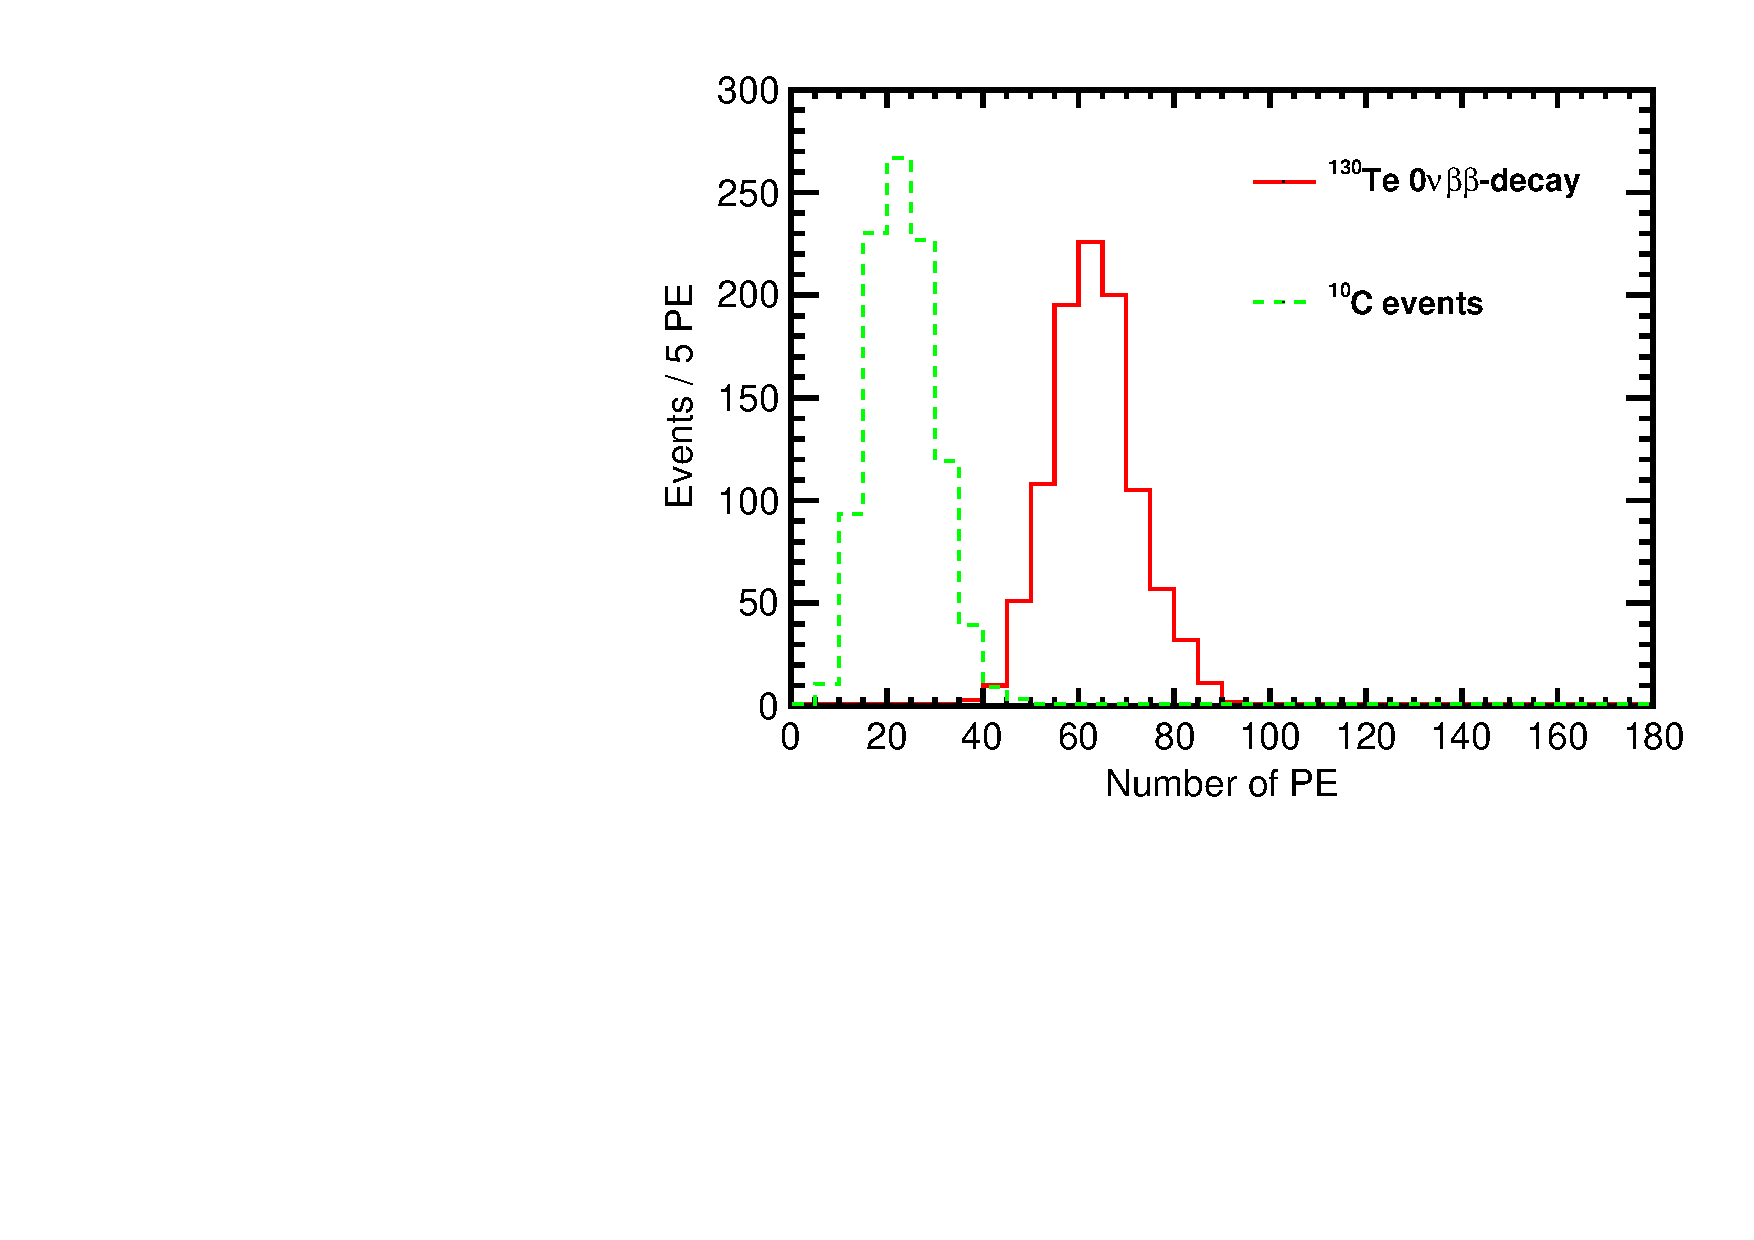
\includegraphics[width=0.95\textwidth]{hMomNPhot_Te130vsC10_allLight_VtxSmear0cm_VtxShiftX0cm_33p5ns_center.pdf}
  \caption{Comparison of total number of early photons between $^{130}$Te 0{\nbb} decay 
    and $^{10}$C events with energy deposition in the range between 2.1 and 2.9~MeV. 
    Events originated at the center of the sphere.
    Perfect vertex reconstruction - true vertex position is used. Time cut of 
    33.5~ns on the photon arrival time is applied.}
\label{fig:NPhot_compare_central}
\end{figure*}


Figure~\ref{fig:NPhot_compare_rndVtx_noSmear} compares total number of PEs for events uniformly 
distributed within the fiducial volume. Perfect knowledge of the vertex is assumed.

\begin{figure*}[ht]
  \centering
  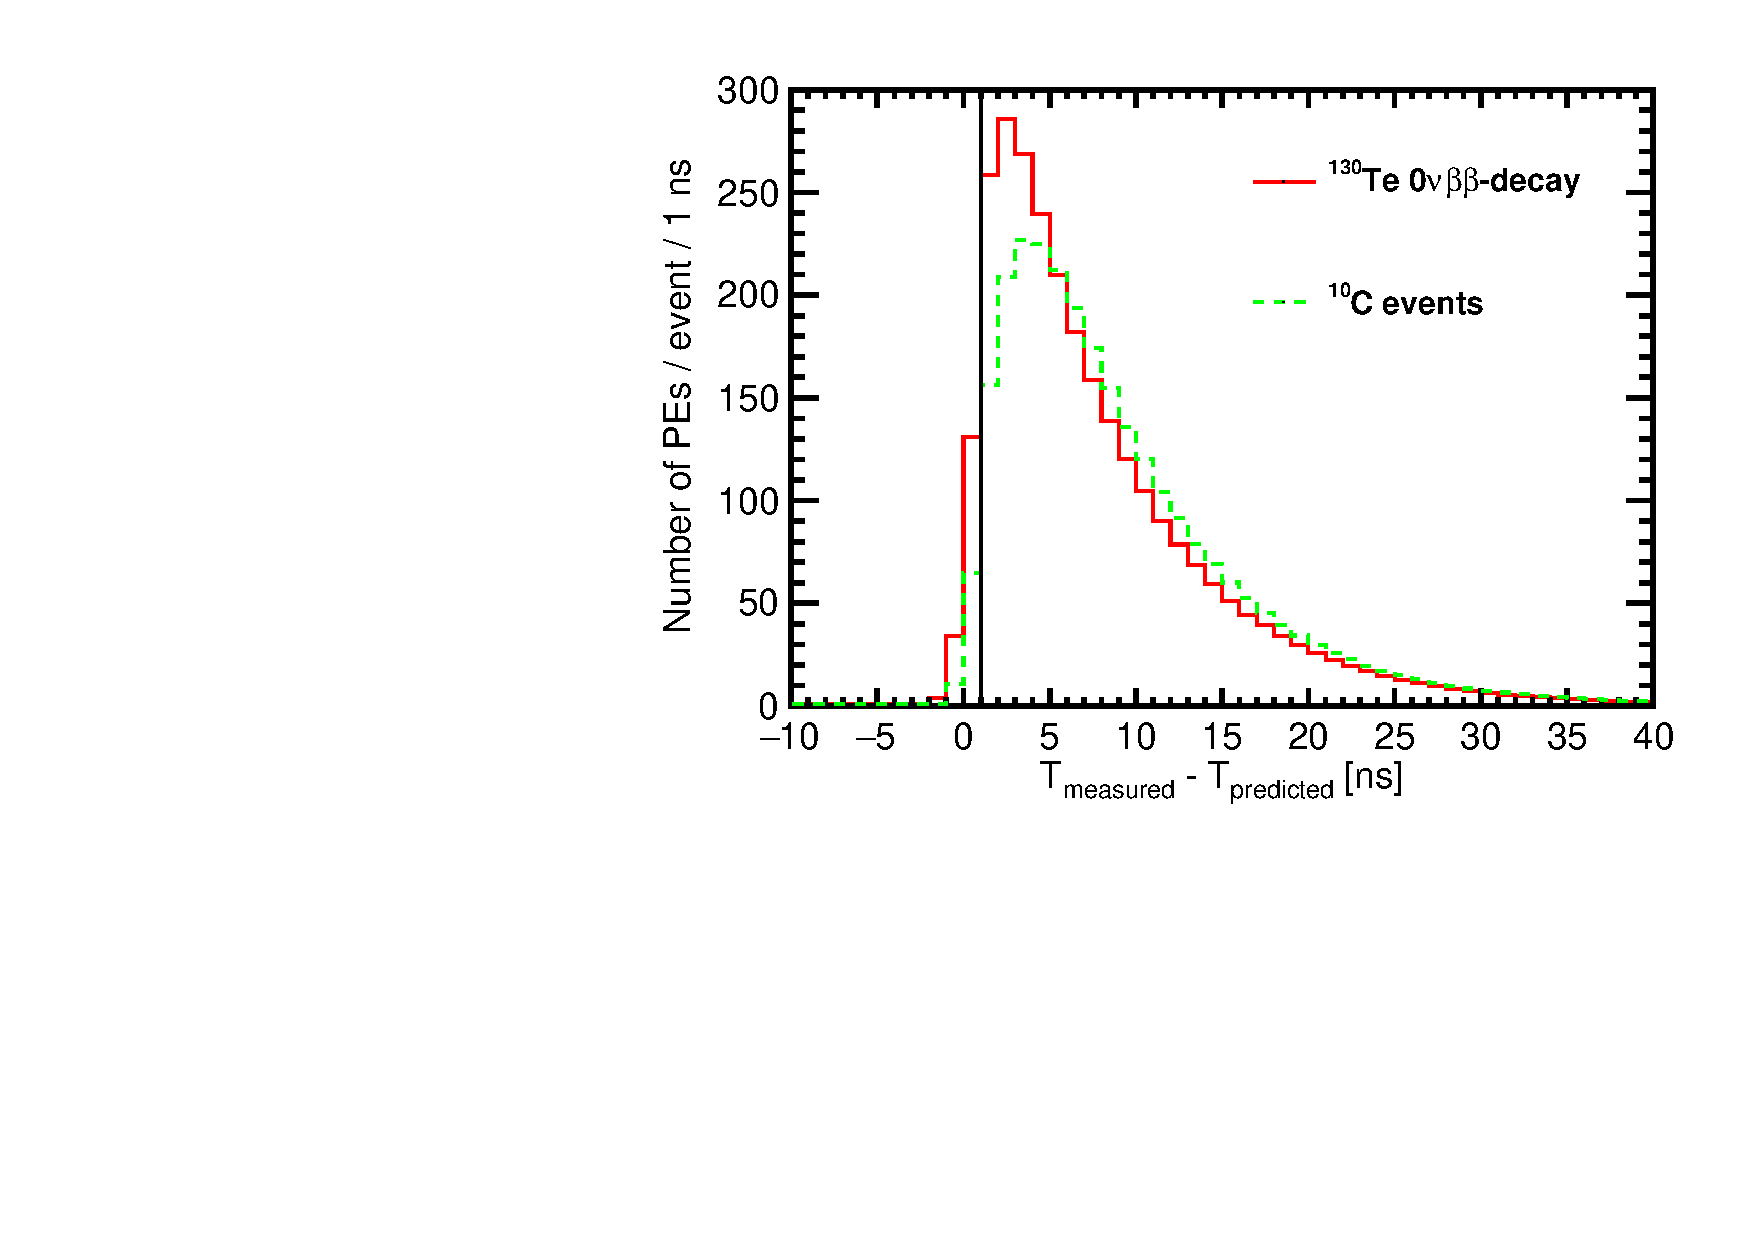
\includegraphics[width=0.45\textwidth]{hMomDT_Te130vsC10_allLight_VtxSmear0cm_VtxShiftX0cm_momDT1p0ns_rndVtx_3p0mSphere.pdf}
  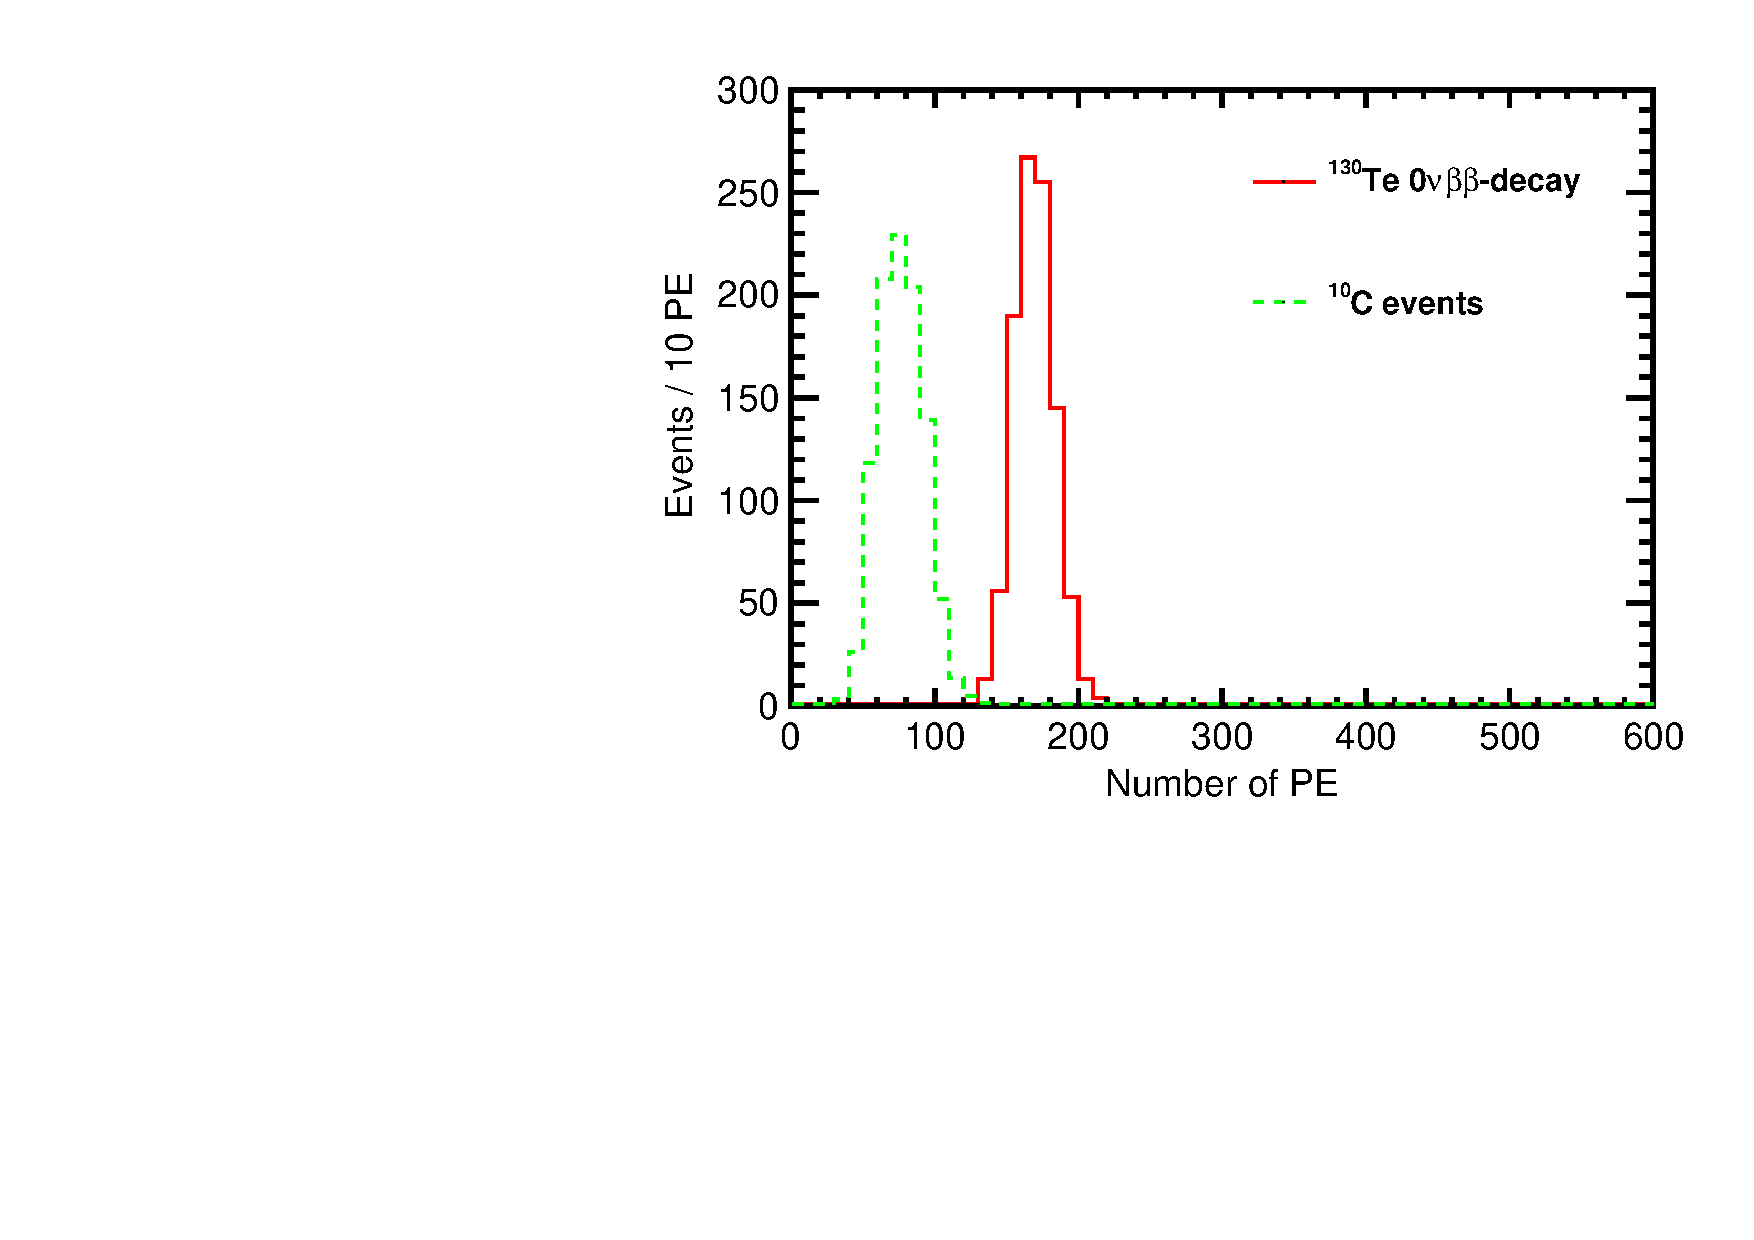
\includegraphics[width=0.45\textwidth]{hMomNPhot_Te130vsC10_allLight_VtxSmear0cm_VtxShiftX0cm_momDT1p0ns_rndVtx_3p0mSphere.pdf}
  \caption{(Left) Difference between measured PE arrival time and arrival time prediction based on 
	vertex location (T$^{predicted} = |r_{hit} - r_{vtx}|/v_{phot}$, where $v_phot = c/1.53$).
        $\vbb$-decay (black solid line) and $\Cten$ events (magenta dashed line) are compared. 
	Vertical line at 1~ns indicates cut for early light selection. 
        (Right) Total number of PEs in the early light sample. 
        $^{10}$C events with energy deposition in the range between 2.1 and 2.9~MeV are
	selected. Verticies are uniformly distributed within the fiducial volume, $R<3$~m.
        {\bf Perfect vertex reconstruction - true vertex position is used.}}
\label{fig:NPhot_compare_rndVtx_noSmear}
\end{figure*}


Figure~\ref{fig:NPhot_compare_rndVtx_Smear3cm} compares total number of PEs for events uniformly
distributed within the fiducial volume and reconstructed vertex smeared with 3~cm resolution.

\begin{figure*}[ht]
  \centering
  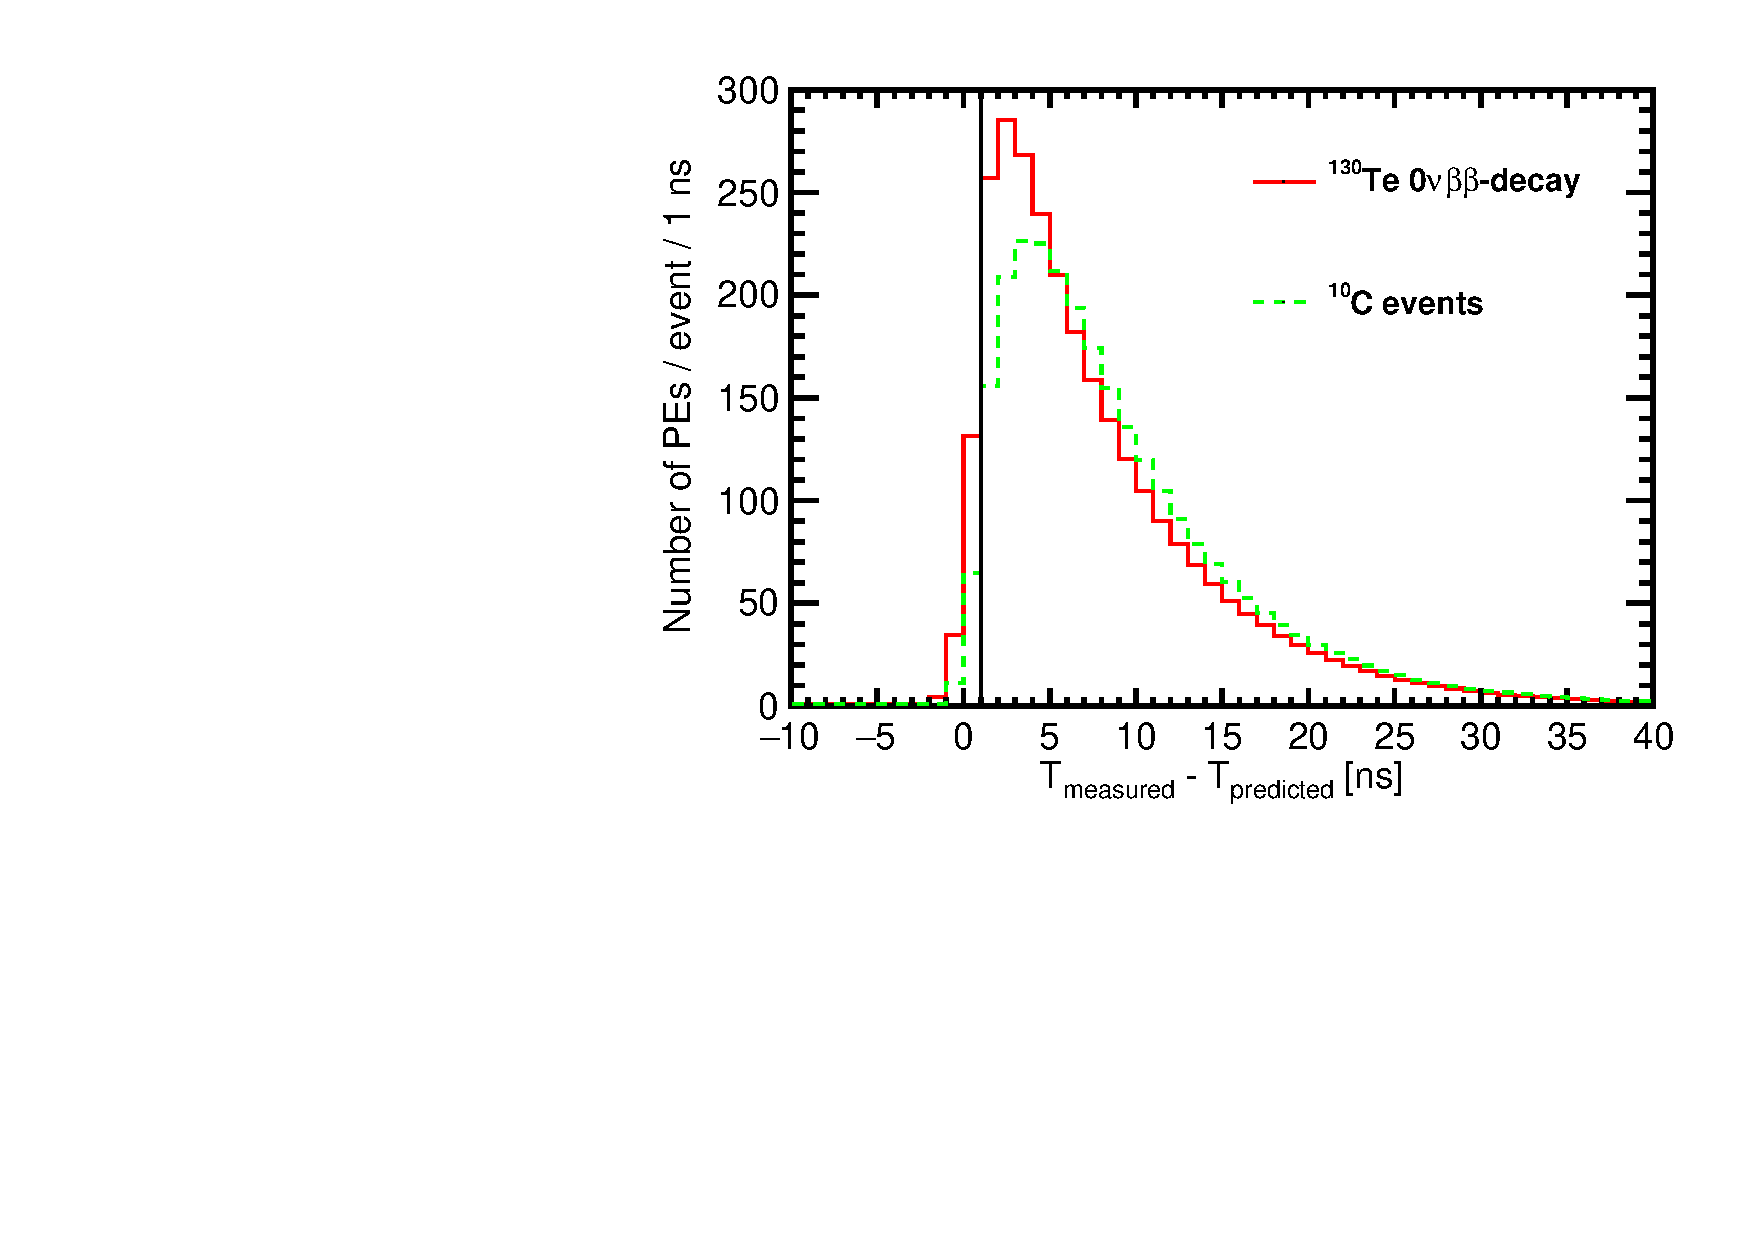
\includegraphics[width=0.45\textwidth]{hMomDT_Te130vsC10_allLight_VtxSmear3cm_VtxShiftX0cm_momDT1p0ns_rndVtx_3p0mSphere.pdf}
  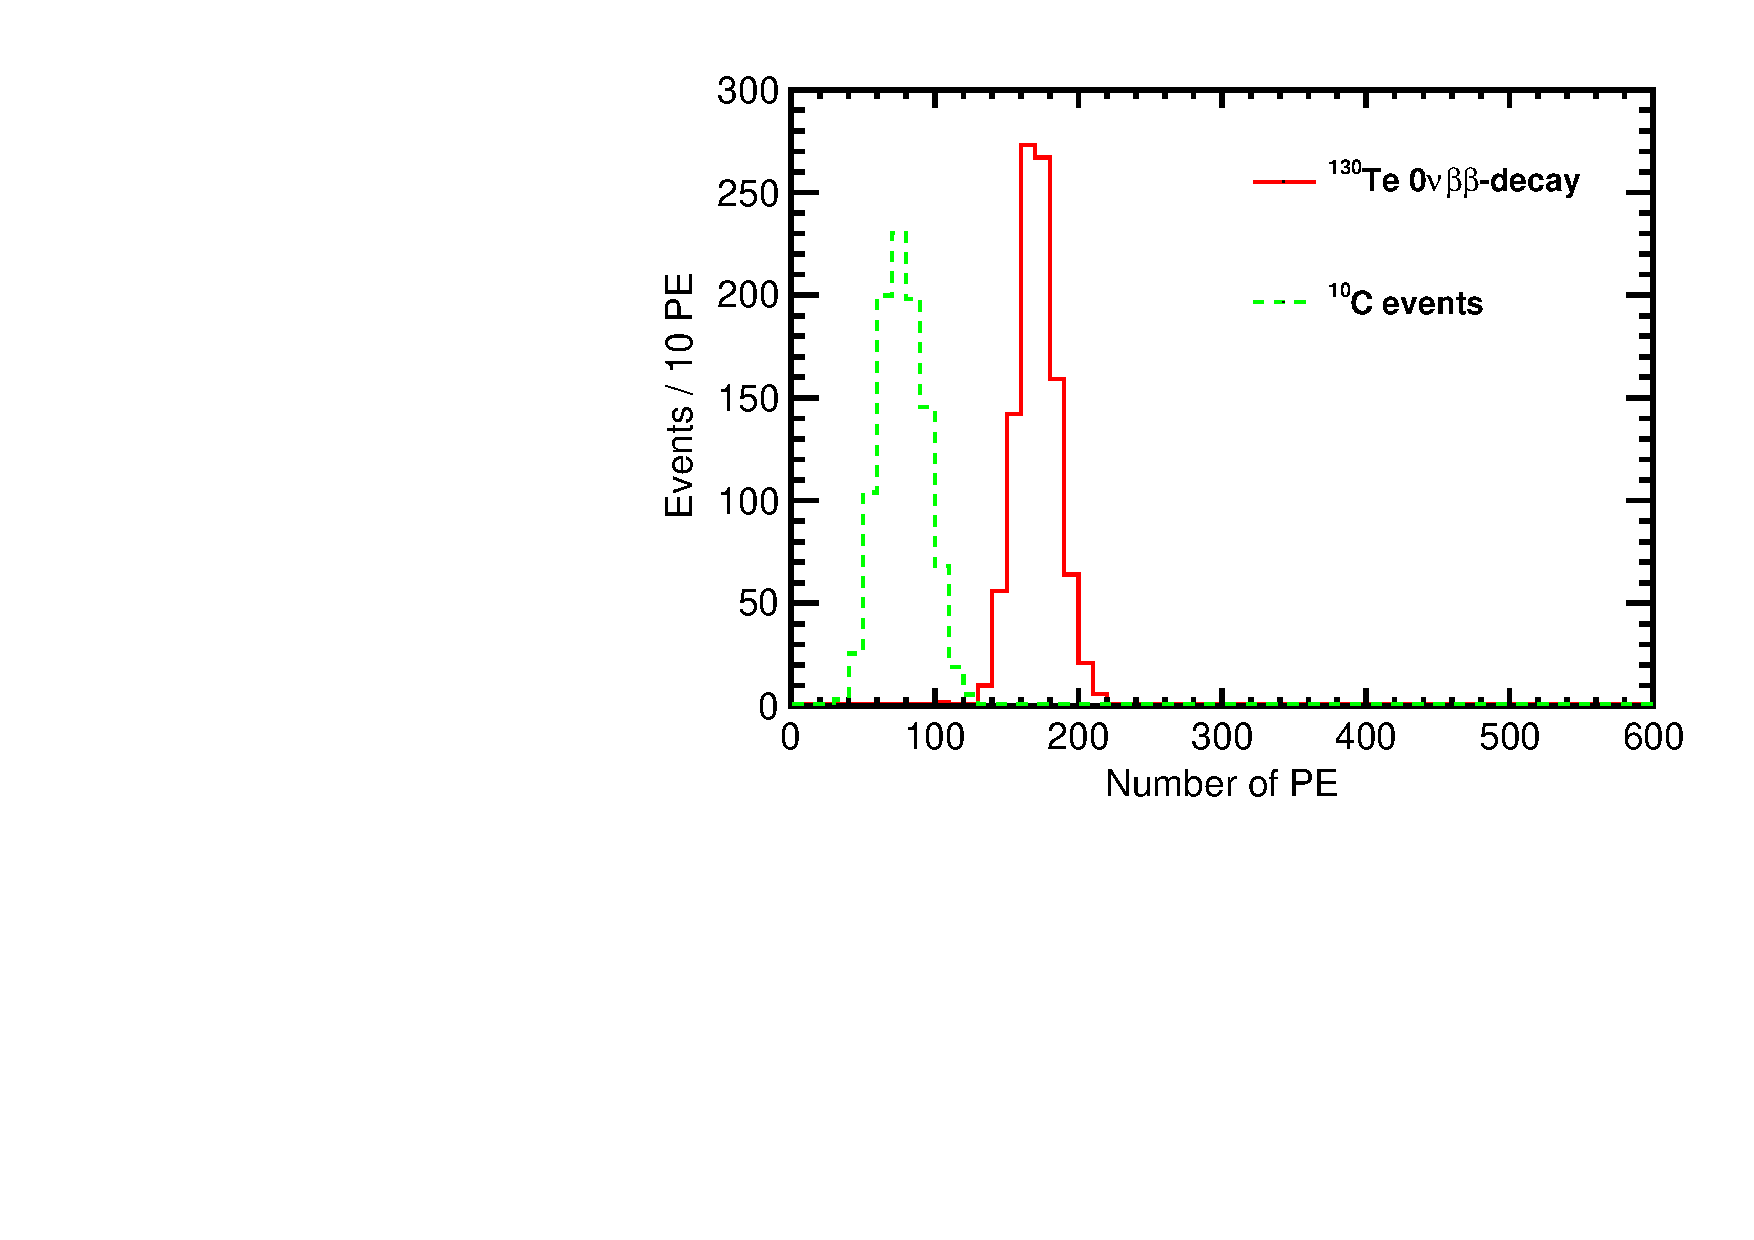
\includegraphics[width=0.45\textwidth]{hMomNPhot_Te130vsC10_allLight_VtxSmear3cm_VtxShiftX0cm_momDT1p0ns_rndVtx_3p0mSphere.pdf}
  \caption{(Left) Difference between measured PE arrival time and arrival time prediction based on
        vertex location (T$^{predicted} = |r_{hit} - r_{vtx}|/v_{phot}$, where $v_phot = c/1.53$).
        $\vbb$-decay (black solid line) and $\Cten$ events (magenta dashed line) are compared.
        Vertical line at 1~ns indicates cut for early light selection.
        (Right) Total number of PEs in the early light sample.
        $^{10}$C events with energy deposition in the range between 2.1 and 2.9~MeV are
        selected. Verticies are uniformly distributed within the fiducial volume, $R<3$~m.
        {\bf Vetrex is smeared with 3~cm resolution.}}
\label{fig:NPhot_compare_rndVtx_Smear3cm}
\end{figure*}


Figure~\ref{fig:NPhot_compare_rndVtx_Smear10cm} compares total number of PEs for events uniformly
distributed within the fiducial volume and reconstructed vertex smeared with 10~cm resolution.

\begin{figure*}[ht]
  \centering
  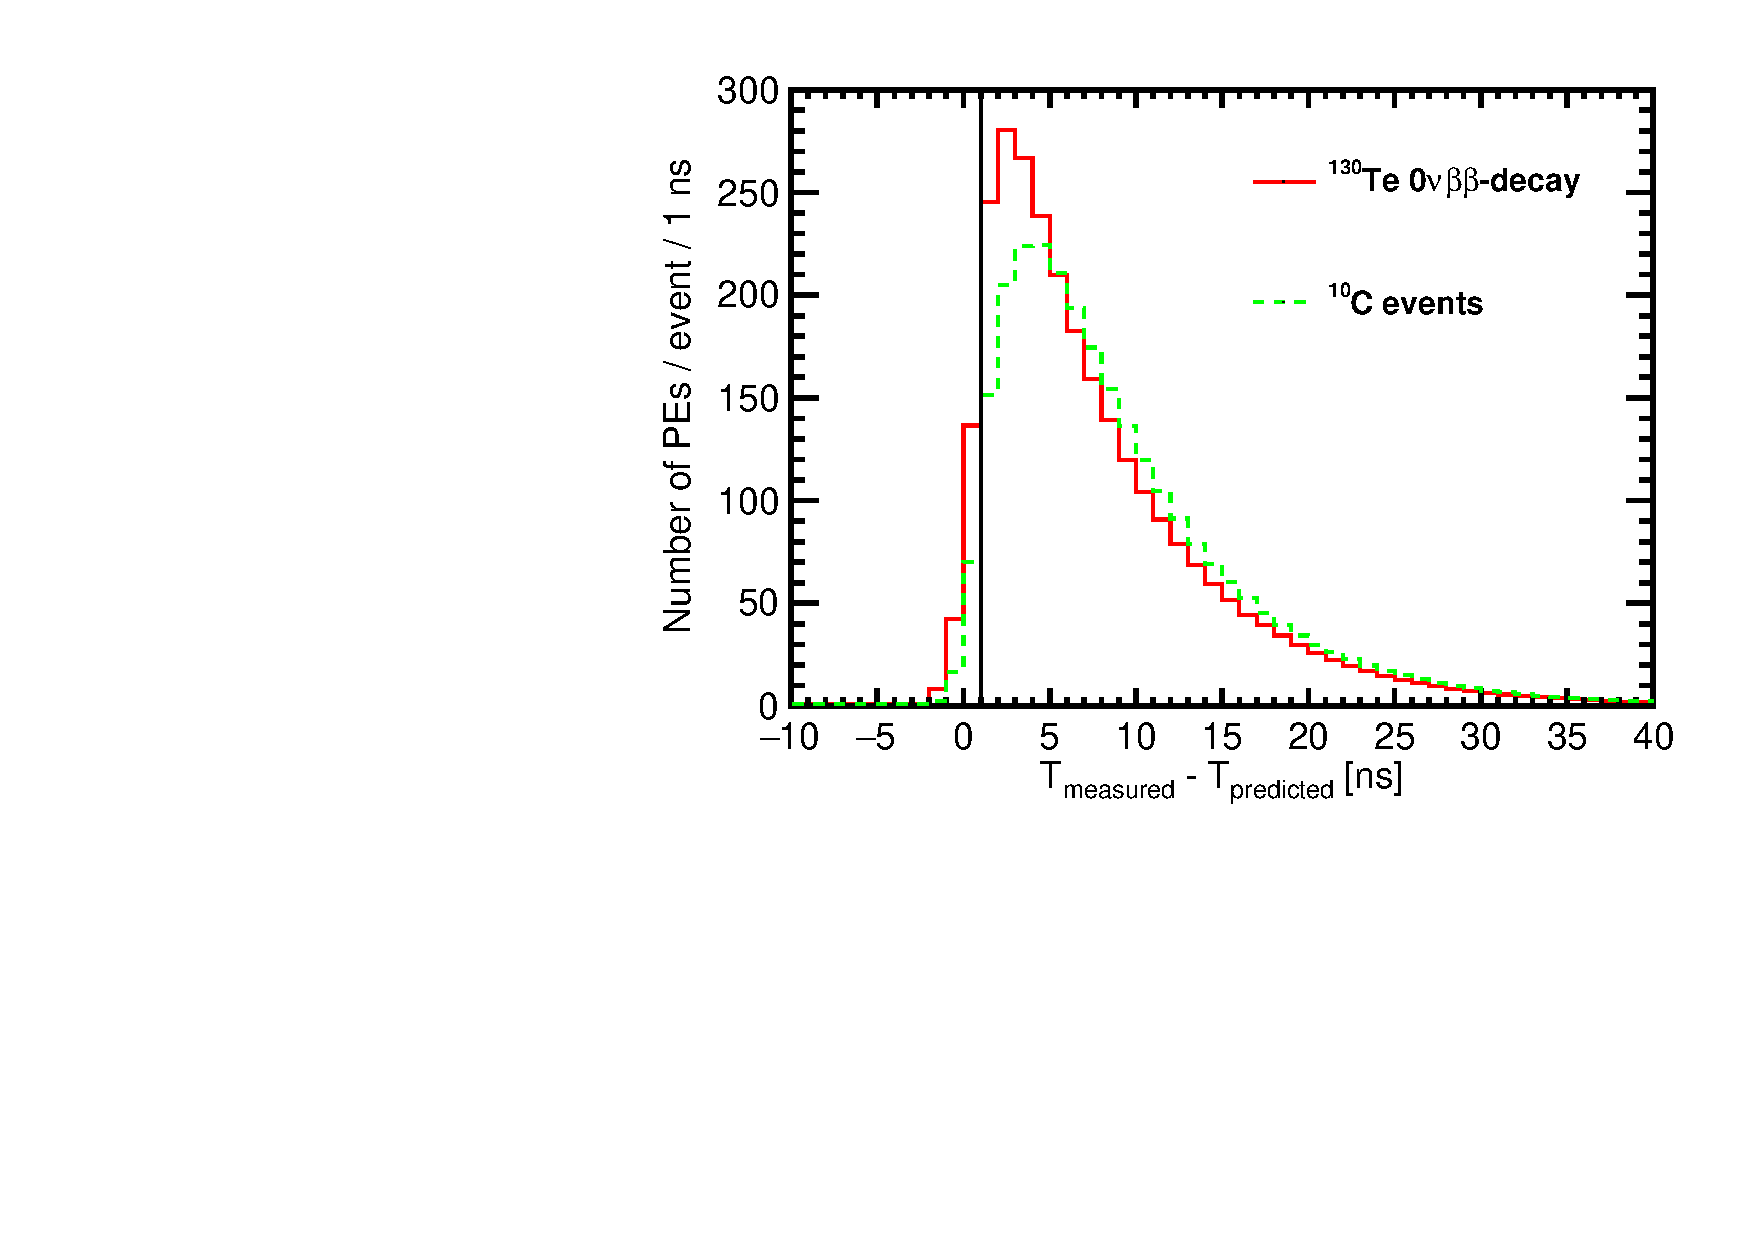
\includegraphics[width=0.45\textwidth]{hMomDT_Te130vsC10_allLight_VtxSmear10cm_VtxShiftX0cm_momDT1p0ns_rndVtx_3p0mSphere.pdf}
  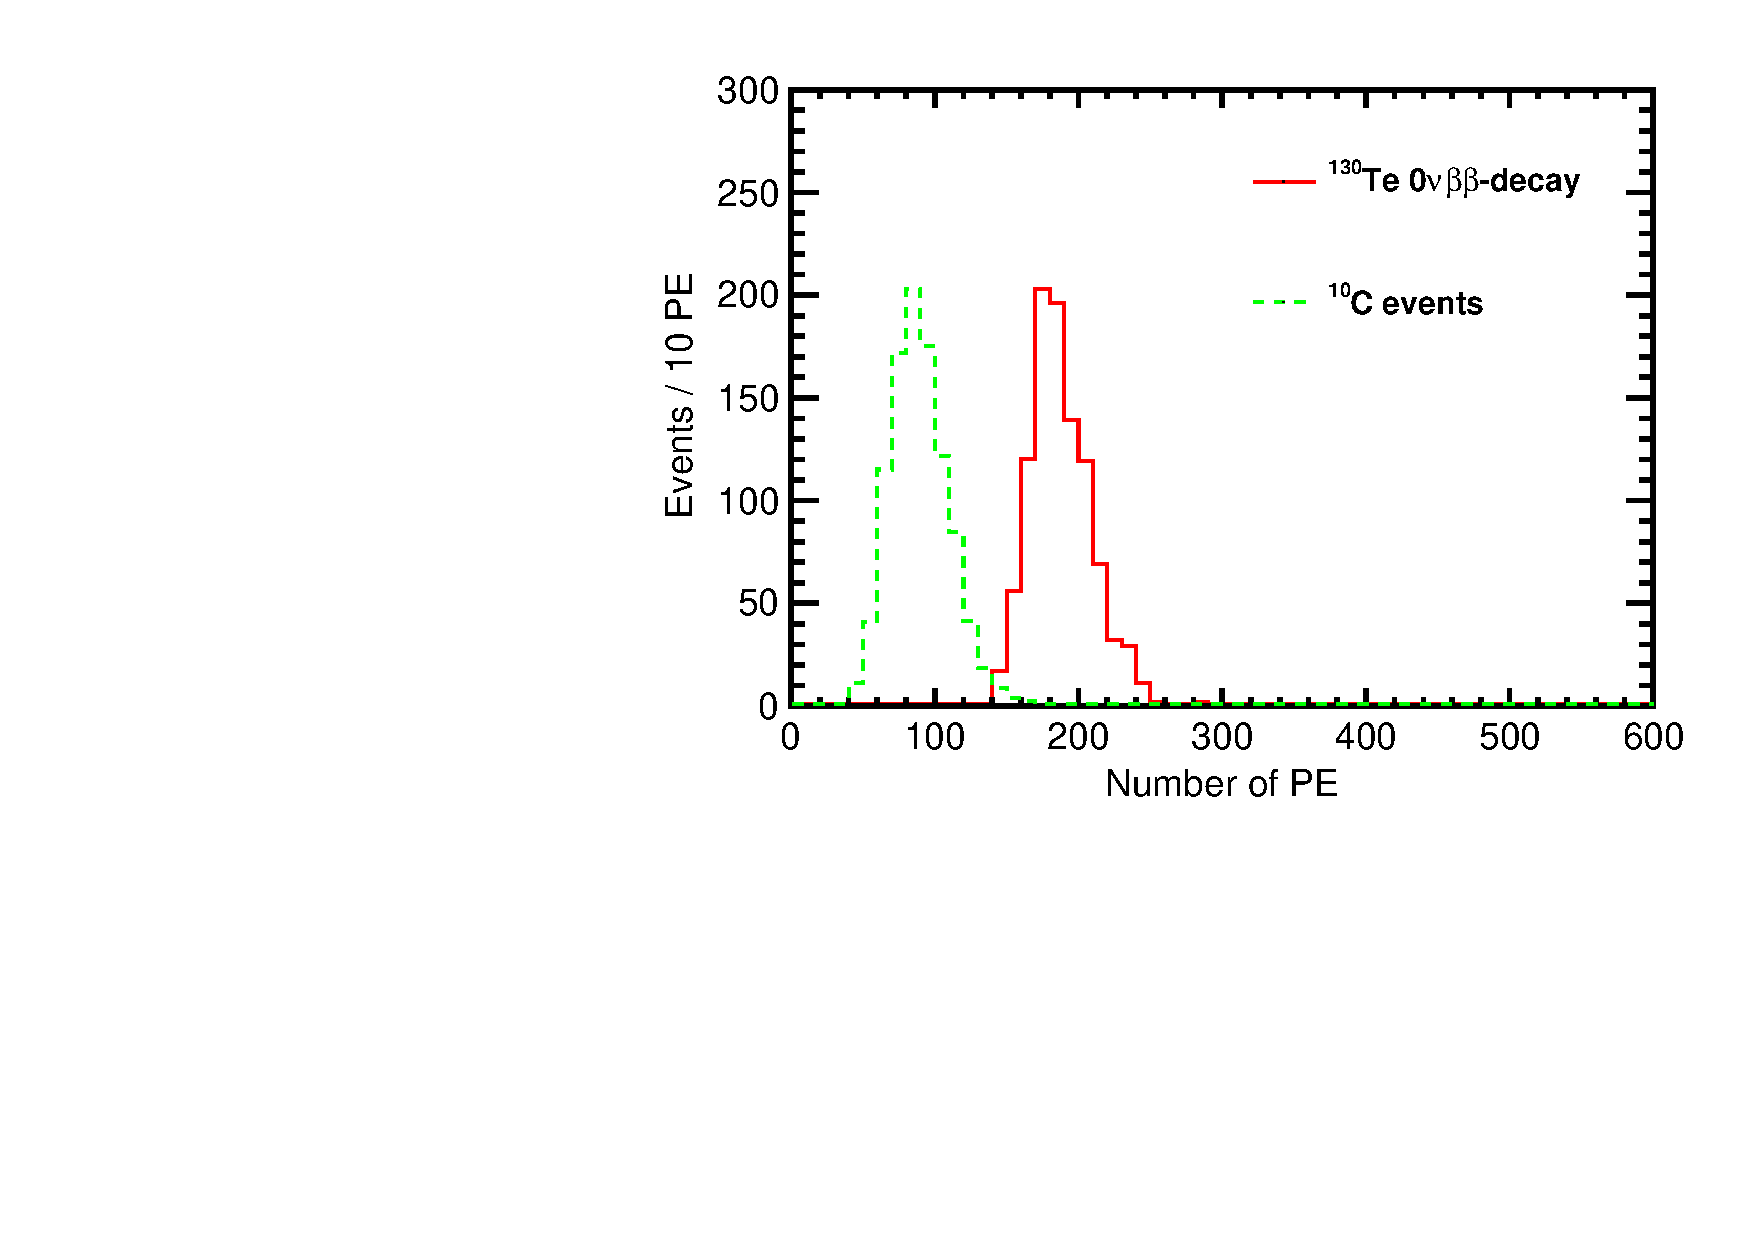
\includegraphics[width=0.45\textwidth]{hMomNPhot_Te130vsC10_allLight_VtxSmear10cm_VtxShiftX0cm_momDT1p0ns_rndVtx_3p0mSphere.pdf}
  \caption{(Left) Difference between measured PE arrival time and arrival time prediction based on
        vertex location (T$^{predicted} = |r_{hit} - r_{vtx}|/v_{phot}$, where $v_phot = c/1.53$).
        $\vbb$-decay (black solid line) and $\Cten$ events (magenta dashed line) are compared.
        Vertical line at 1~ns indicates cut for early light selection.
        (Right) Total number of PEs in the early light sample.
        $^{10}$C events with energy deposition in the range between 2.1 and 2.9~MeV are
        selected. Verticies are uniformly distributed within the fiducial volume, $R<3$~m.
        {\bf Vetrex is smeared with 10~cm resolution.}}
\label{fig:NPhot_compare_rndVtx_Smear10cm}
\end{figure*}



Figure~\ref{fig:NPhot_compare_rndVtx_Smear30cm} compares total number of PEs for events uniformly
distributed within the fiducial volume and reconstructed vertex smeared with 30~cm resolution.

\begin{figure*}[ht]
  \centering
  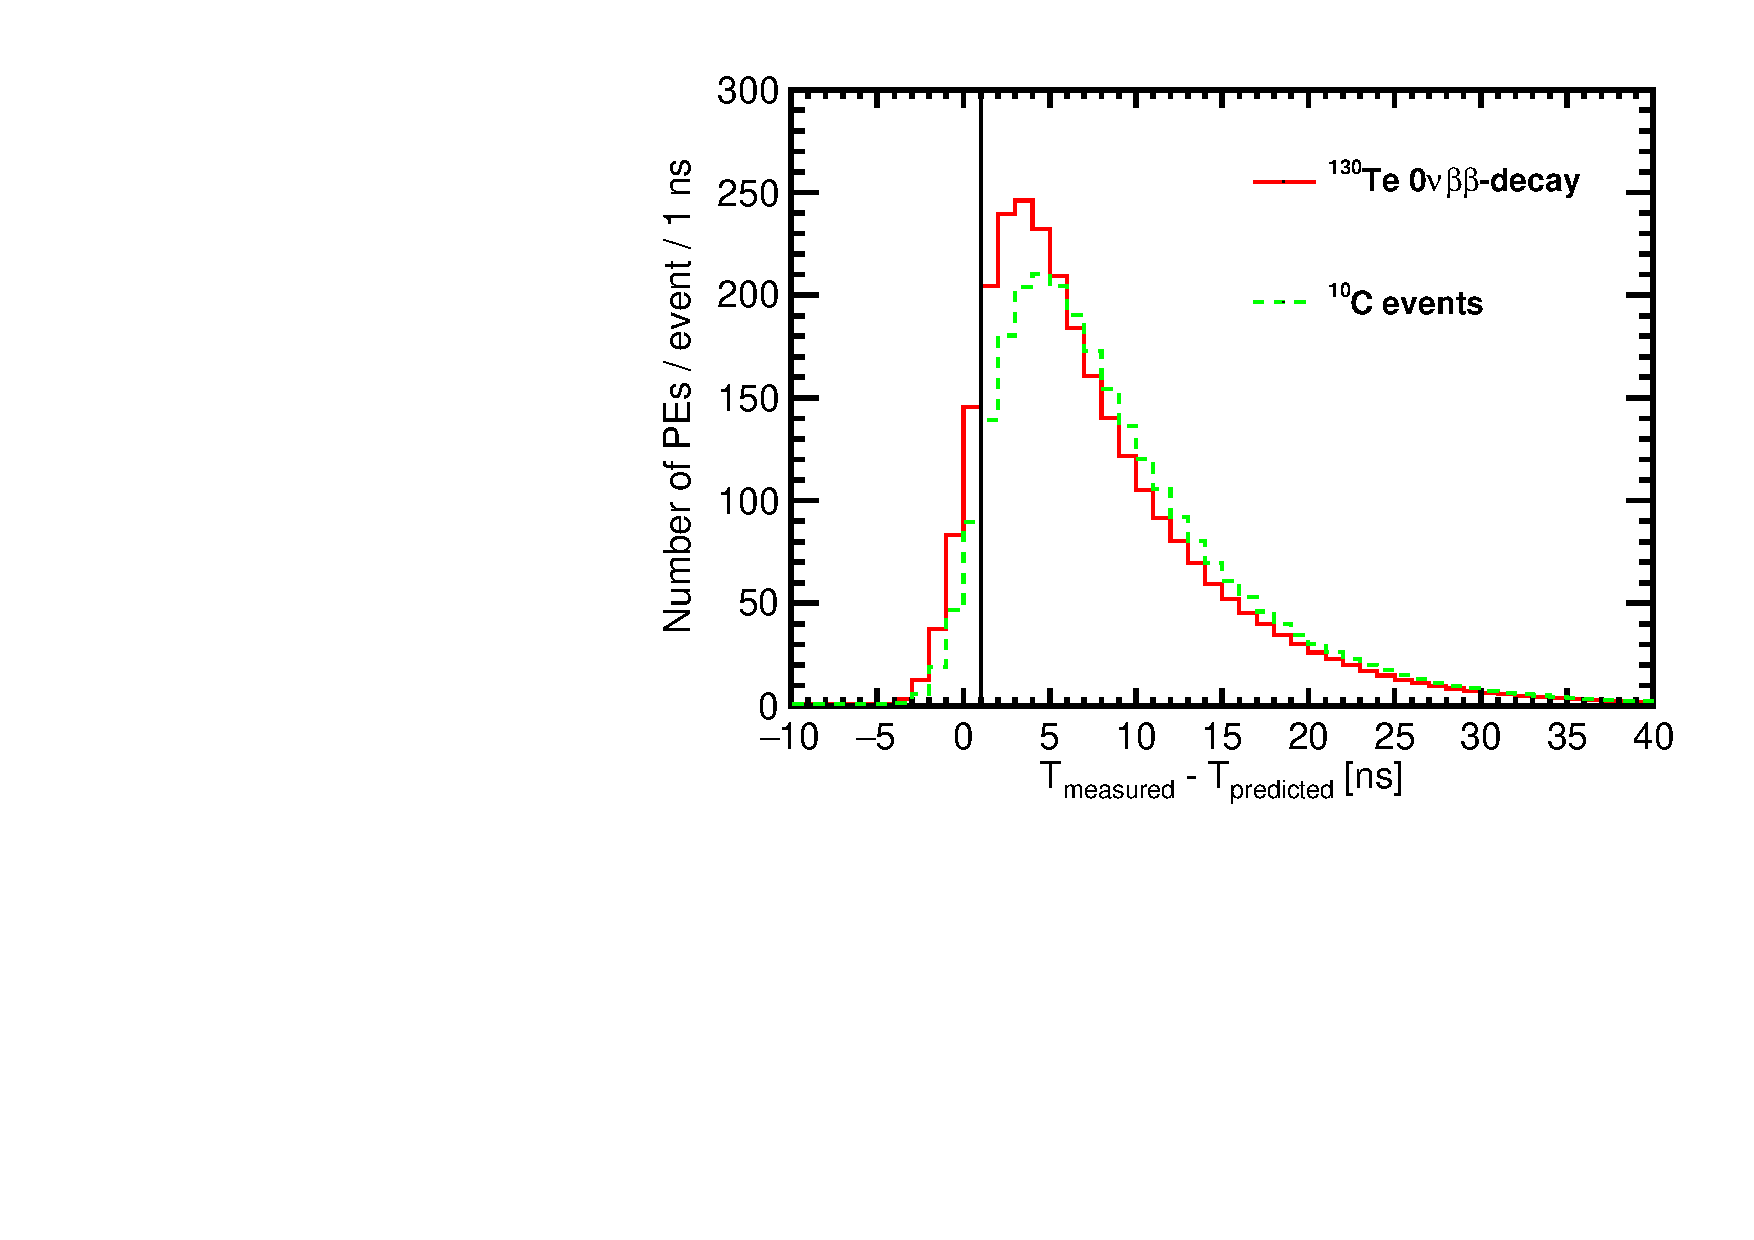
\includegraphics[width=0.45\textwidth]{hMomDT_Te130vsC10_allLight_VtxSmear30cm_VtxShiftX0cm_momDT1p0ns_rndVtx_3p0mSphere.pdf}
  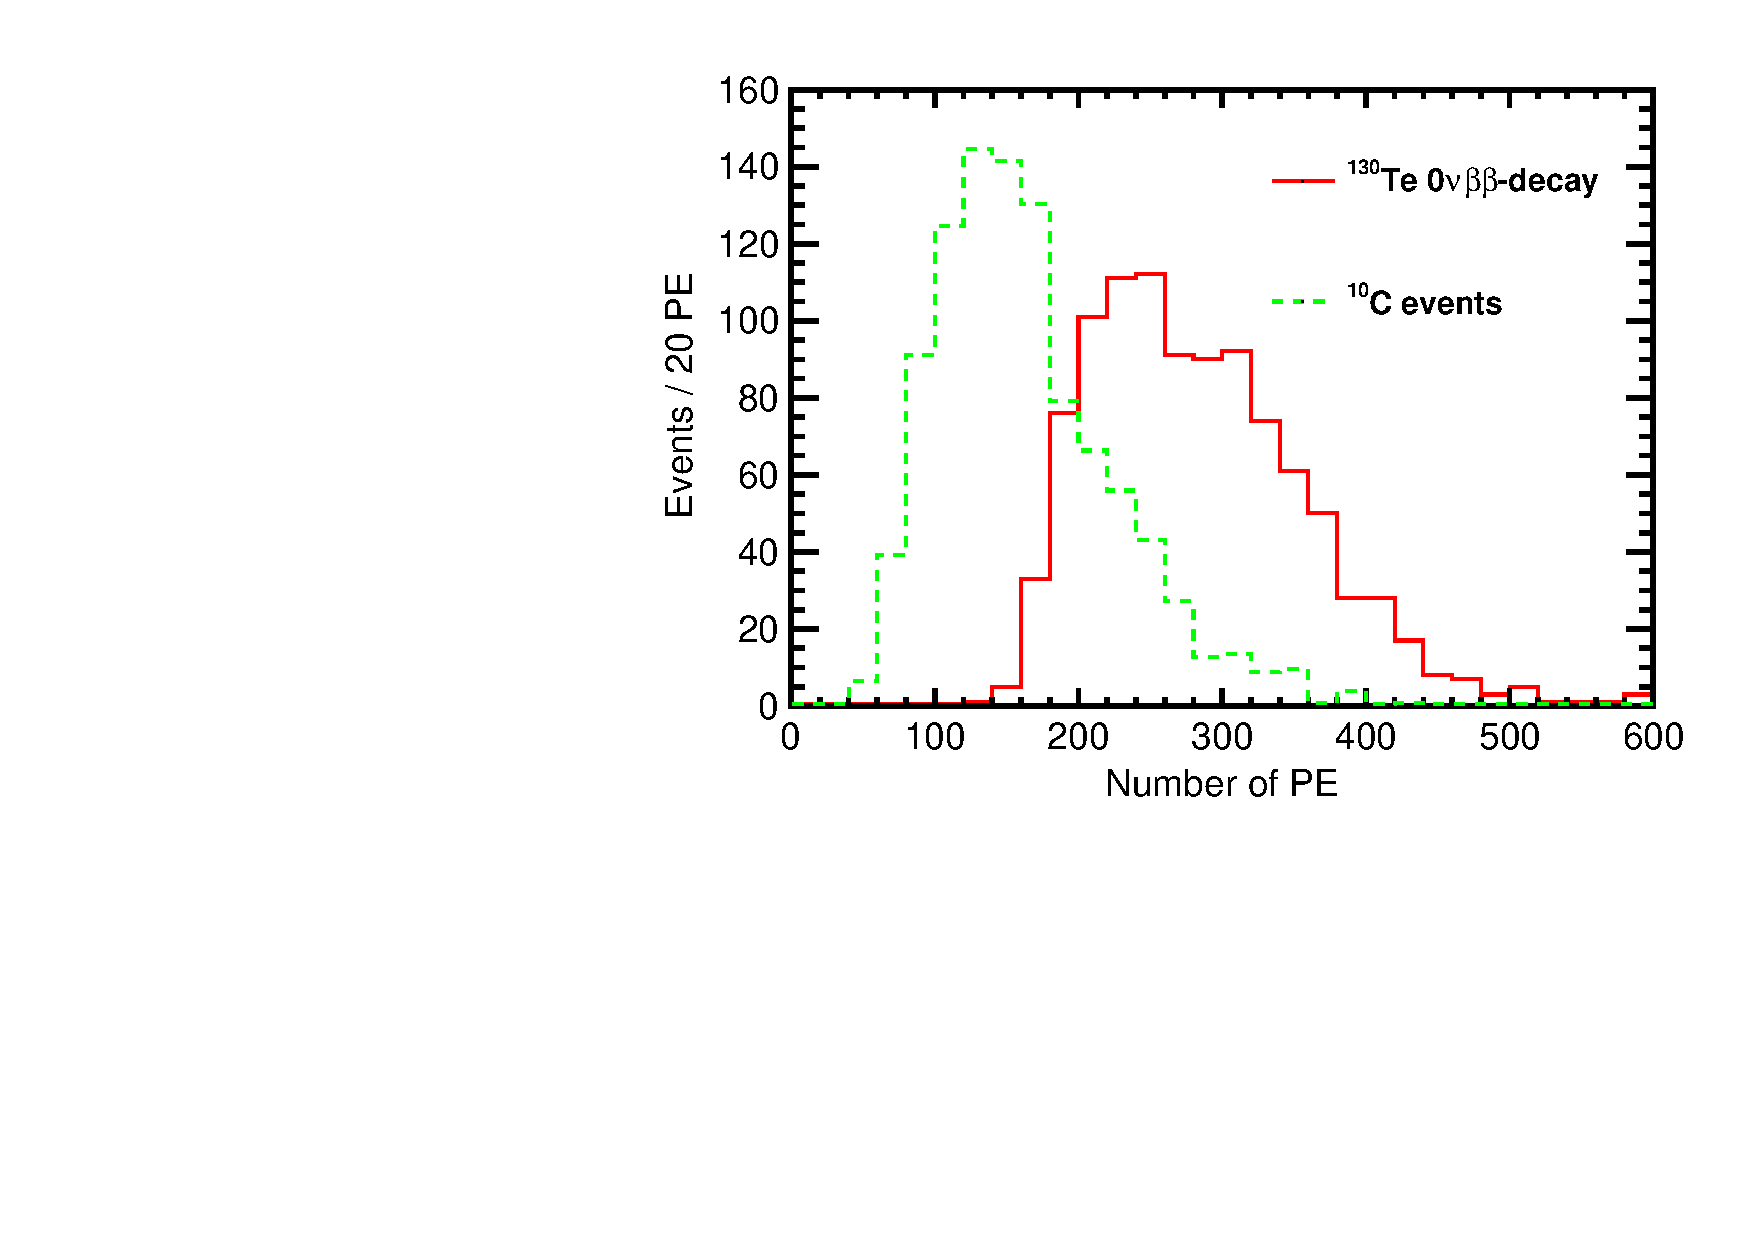
\includegraphics[width=0.45\textwidth]{hMomNPhot_Te130vsC10_allLight_VtxSmear30cm_VtxShiftX0cm_momDT1p0ns_rndVtx_3p0mSphere.pdf}
  \caption{(Left) Difference between measured PE arrival time and arrival time prediction based on
        vertex location (T$^{predicted} = |r_{hit} - r_{vtx}|/v_{phot}$, where $v_phot = c/1.53$).
        $\vbb$-decay (black solid line) and $\Cten$ events (magenta dashed line) are compared.
        Vertical line at 1~ns indicates cut for early light selection.
        (Right) Total number of PEs in the early light sample.
        $^{10}$C events with energy deposition in the range between 2.1 and 2.9~MeV are
        selected. Verticies are uniformly distributed within the fiducial volume, $R<3$~m.
        {\bf Vetrex is smeared with 30~cm resolution.}}
\label{fig:NPhot_compare_rndVtx_Smear30cm}
\end{figure*}


Figure~\ref{fig:NPhot_compare_rndVtx_Smear50cm} compares total number of PEs for events uniformly
distributed within the fiducial volume and reconstructed vertex smeared with 50~cm resolution.

\begin{figure*}[ht]
  \centering
  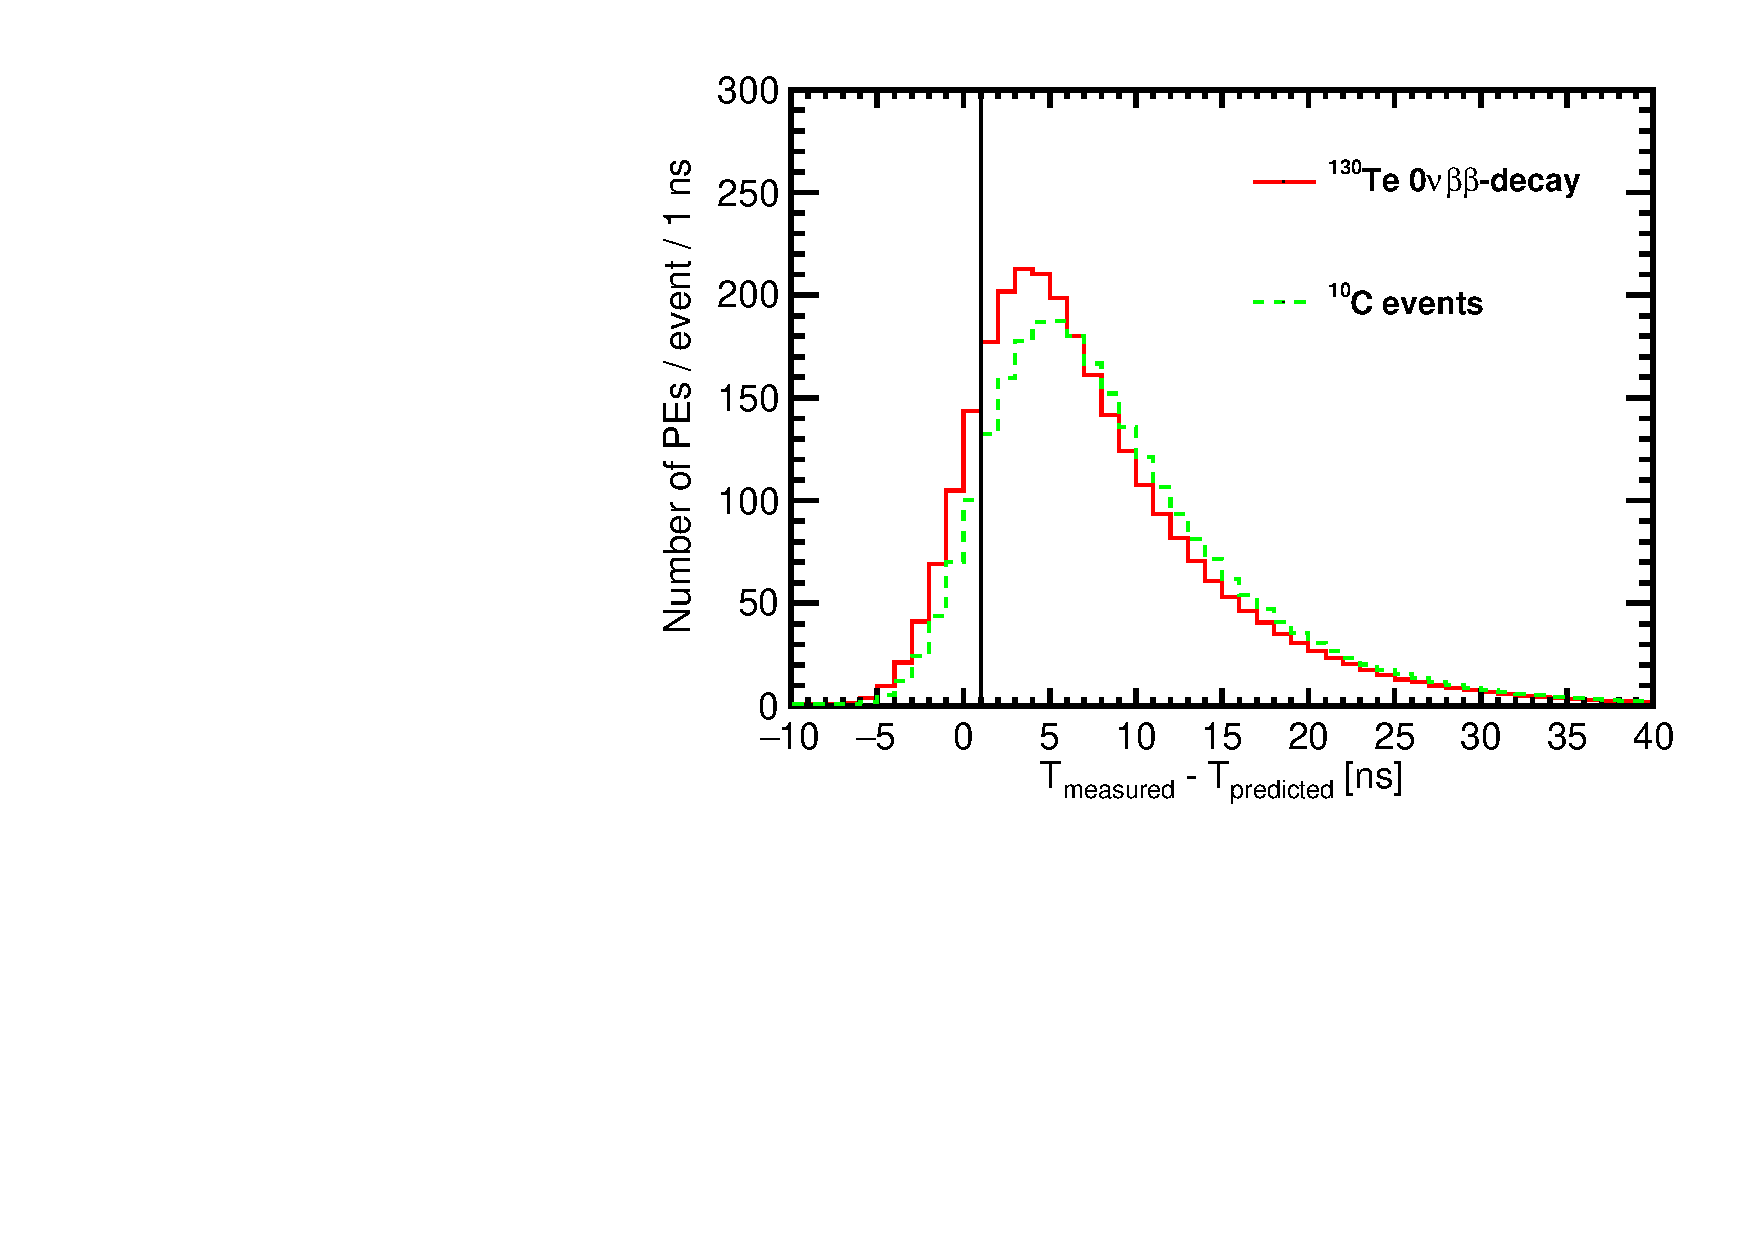
\includegraphics[width=0.45\textwidth]{hMomDT_Te130vsC10_allLight_VtxSmear50cm_VtxShiftX0cm_momDT1p0ns_rndVtx_3p0mSphere.pdf}
  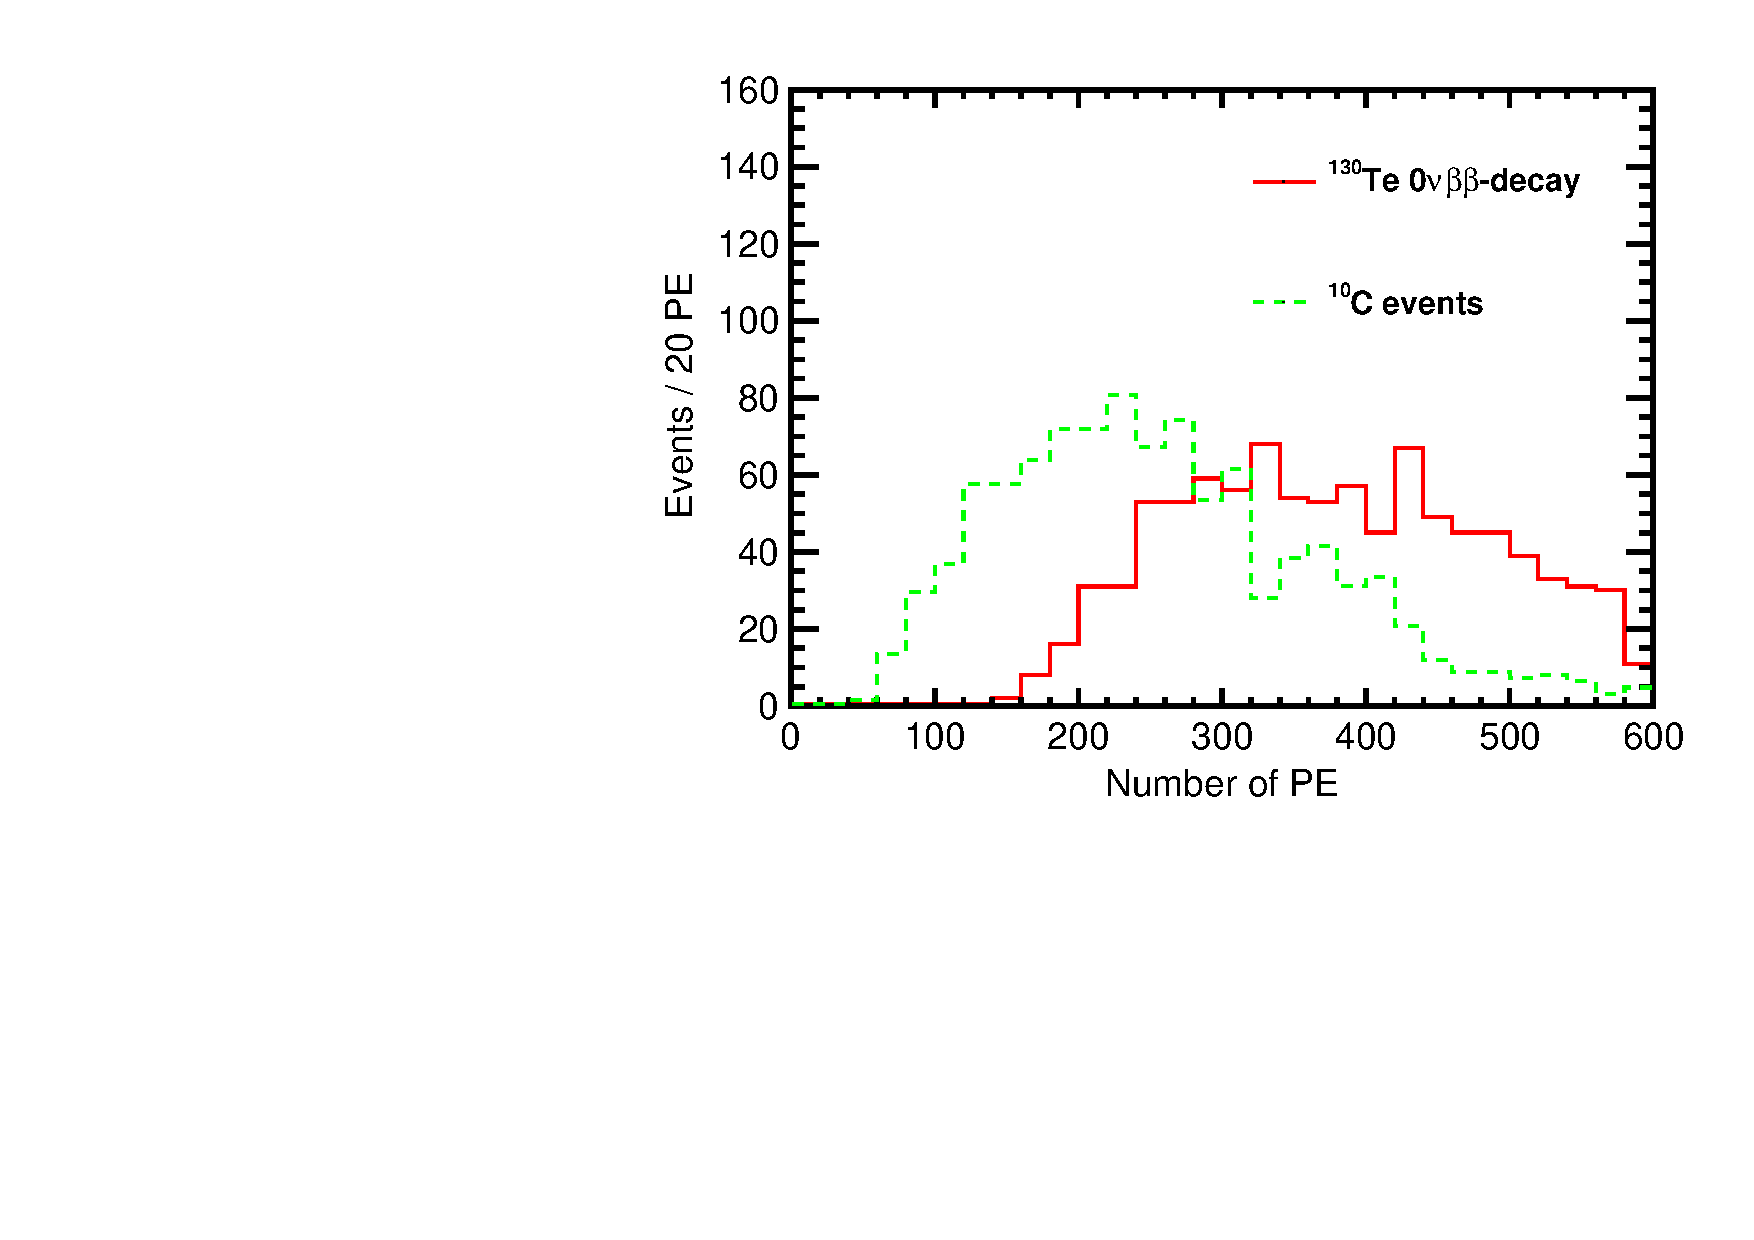
\includegraphics[width=0.45\textwidth]{hMomNPhot_Te130vsC10_allLight_VtxSmear50cm_VtxShiftX0cm_momDT1p0ns_rndVtx_3p0mSphere.pdf}
  \caption{(Left) Difference between measured PE arrival time and arrival time prediction based on
        vertex location (T$^{predicted} = |r_{hit} - r_{vtx}|/v_{phot}$, where $v_phot = c/1.53$).
        $\vbb$-decay (black solid line) and $\Cten$ events (magenta dashed line) are compared.
        Vertical line at 1~ns indicates cut for early light selection.
        (Right) Total number of PEs in the early light sample.
        $^{10}$C events with energy deposition in the range between 2.1 and 2.9~MeV are
        selected. Verticies are uniformly distributed within the fiducial volume, $R<3$~m.
        {\bf Vetrex is smeared with 50~cm resolution.}}
\label{fig:NPhot_compare_rndVtx_Smear50cm}
\end{figure*}



% !!!!!!!!!!!!	Commented text begins	!!!!!!!!!!!!!!!!!!!!!
\begin{comment}
\newpage

\section{0{\nbb} decay vs $^{10}$C background}

Other common backgrounds to 0{\nbb} decay search include radioactive
decays of nuclei that are excited by cosmic muons and produced through the decays of Th and U
naturally present in the materials. In liquid scintillator detectors,
most of events from Th and U decays occur in the materials of
the scintillator enclosure. Typically, they enter the fiducial volume
as 2.6~MeV gammas. These gammas pass into the fiducial volume either because they showered too late or have
mis-reconstructed vertex. Both effects depend on details of a
particular experiment and in this paper we make no attempt
to introduce a topology reconstruction for the backgrounds coming from
Th and U lines. Cosmic induced backgrounds, to the contrary, are more
generic and originate inside the fiducial volume. In this section we
discuss event topology of $^{10}$C events that are most relevant in the
energy of 2-3~MeV.

Typical energy deposition by $^{10}$C events is shown in
Fig.~\ref{fig:Edep_C10}. We propose to use spherical harmonics
analysis to separate 0{\nbb} decay events from $^{10}$C events that
within energy resolution overlap with the 0{\nbb} decay Q-value.

\begin{figure}[h]
  \centering
  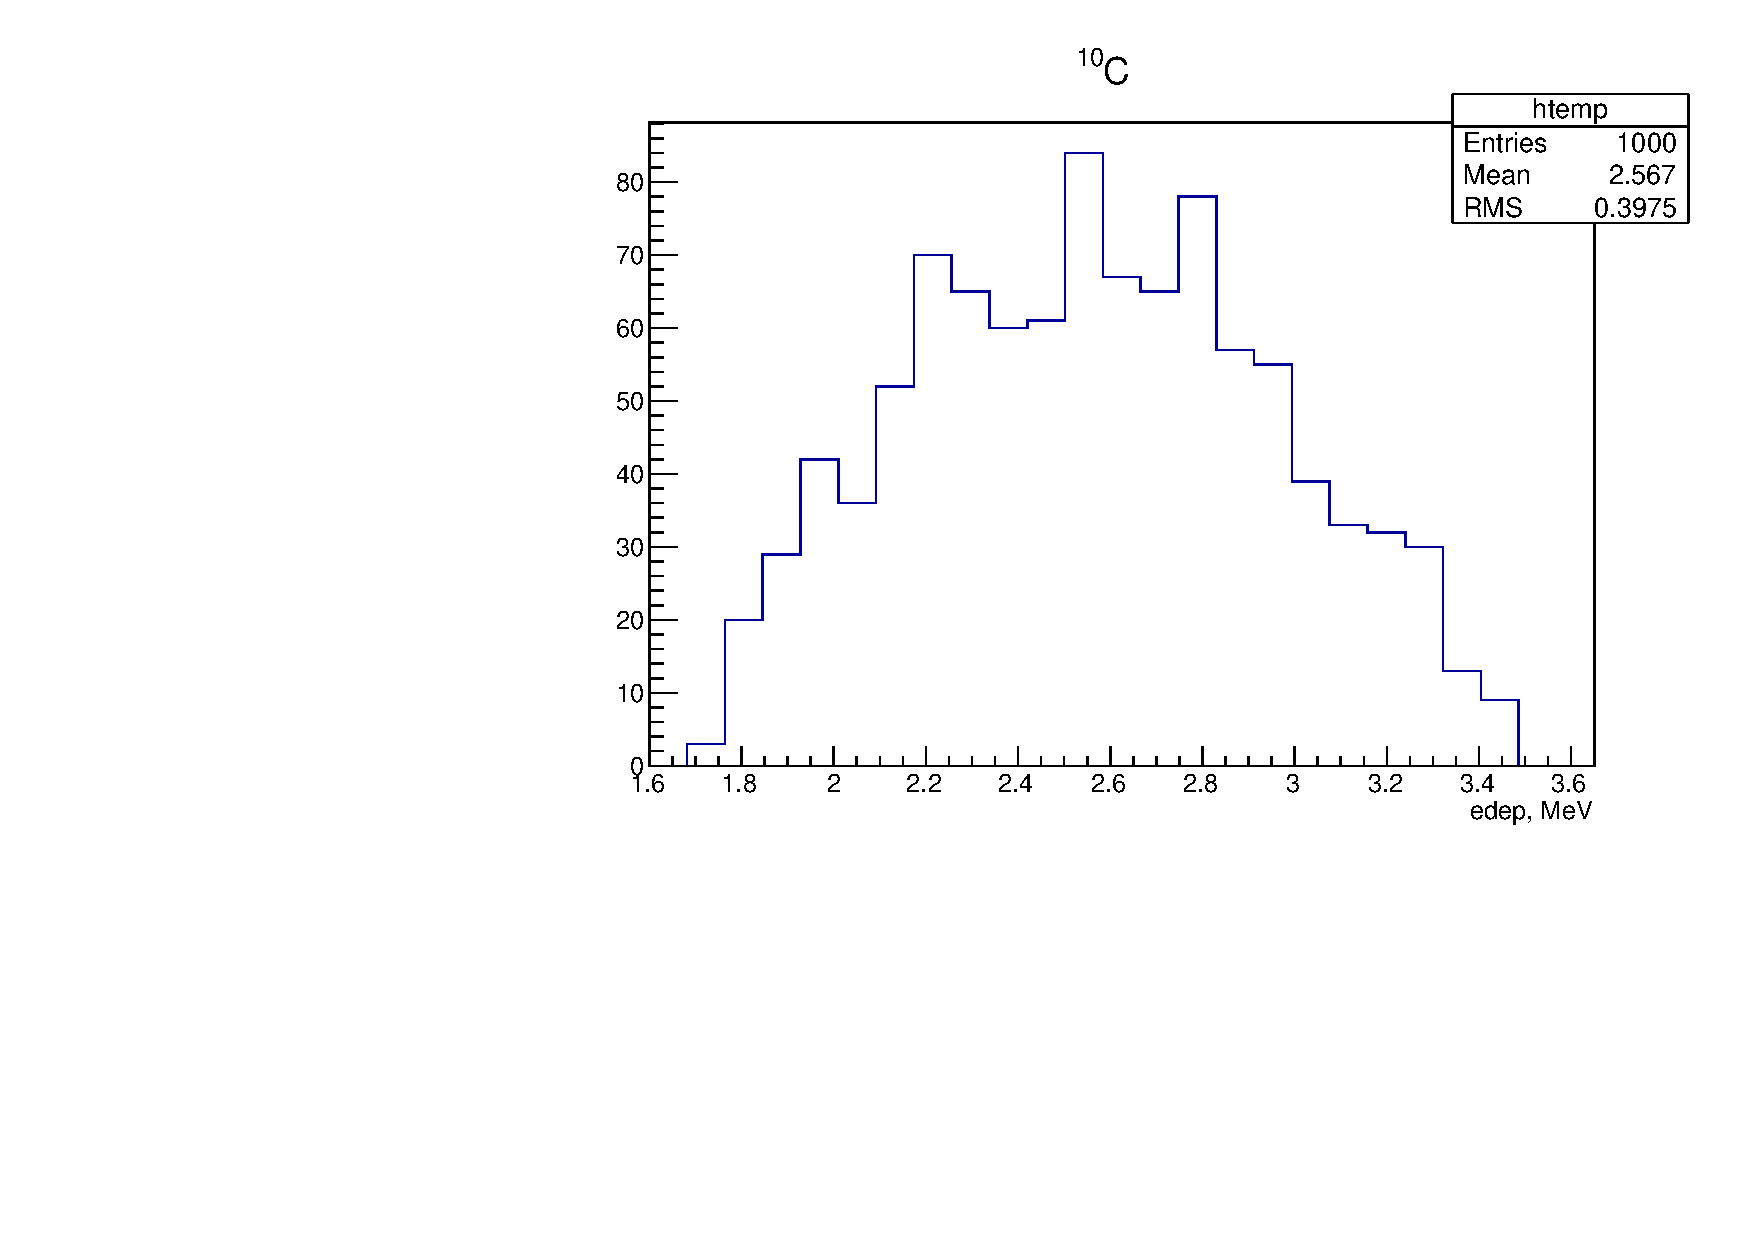
\includegraphics[width=0.95\textwidth]{hEdep_C10.pdf}
  \caption{Energy deposition in $^{10}$C events.}
  \label{fig:Edep_C10}
\end{figure}

\begin{figure}[h]
  \centering
  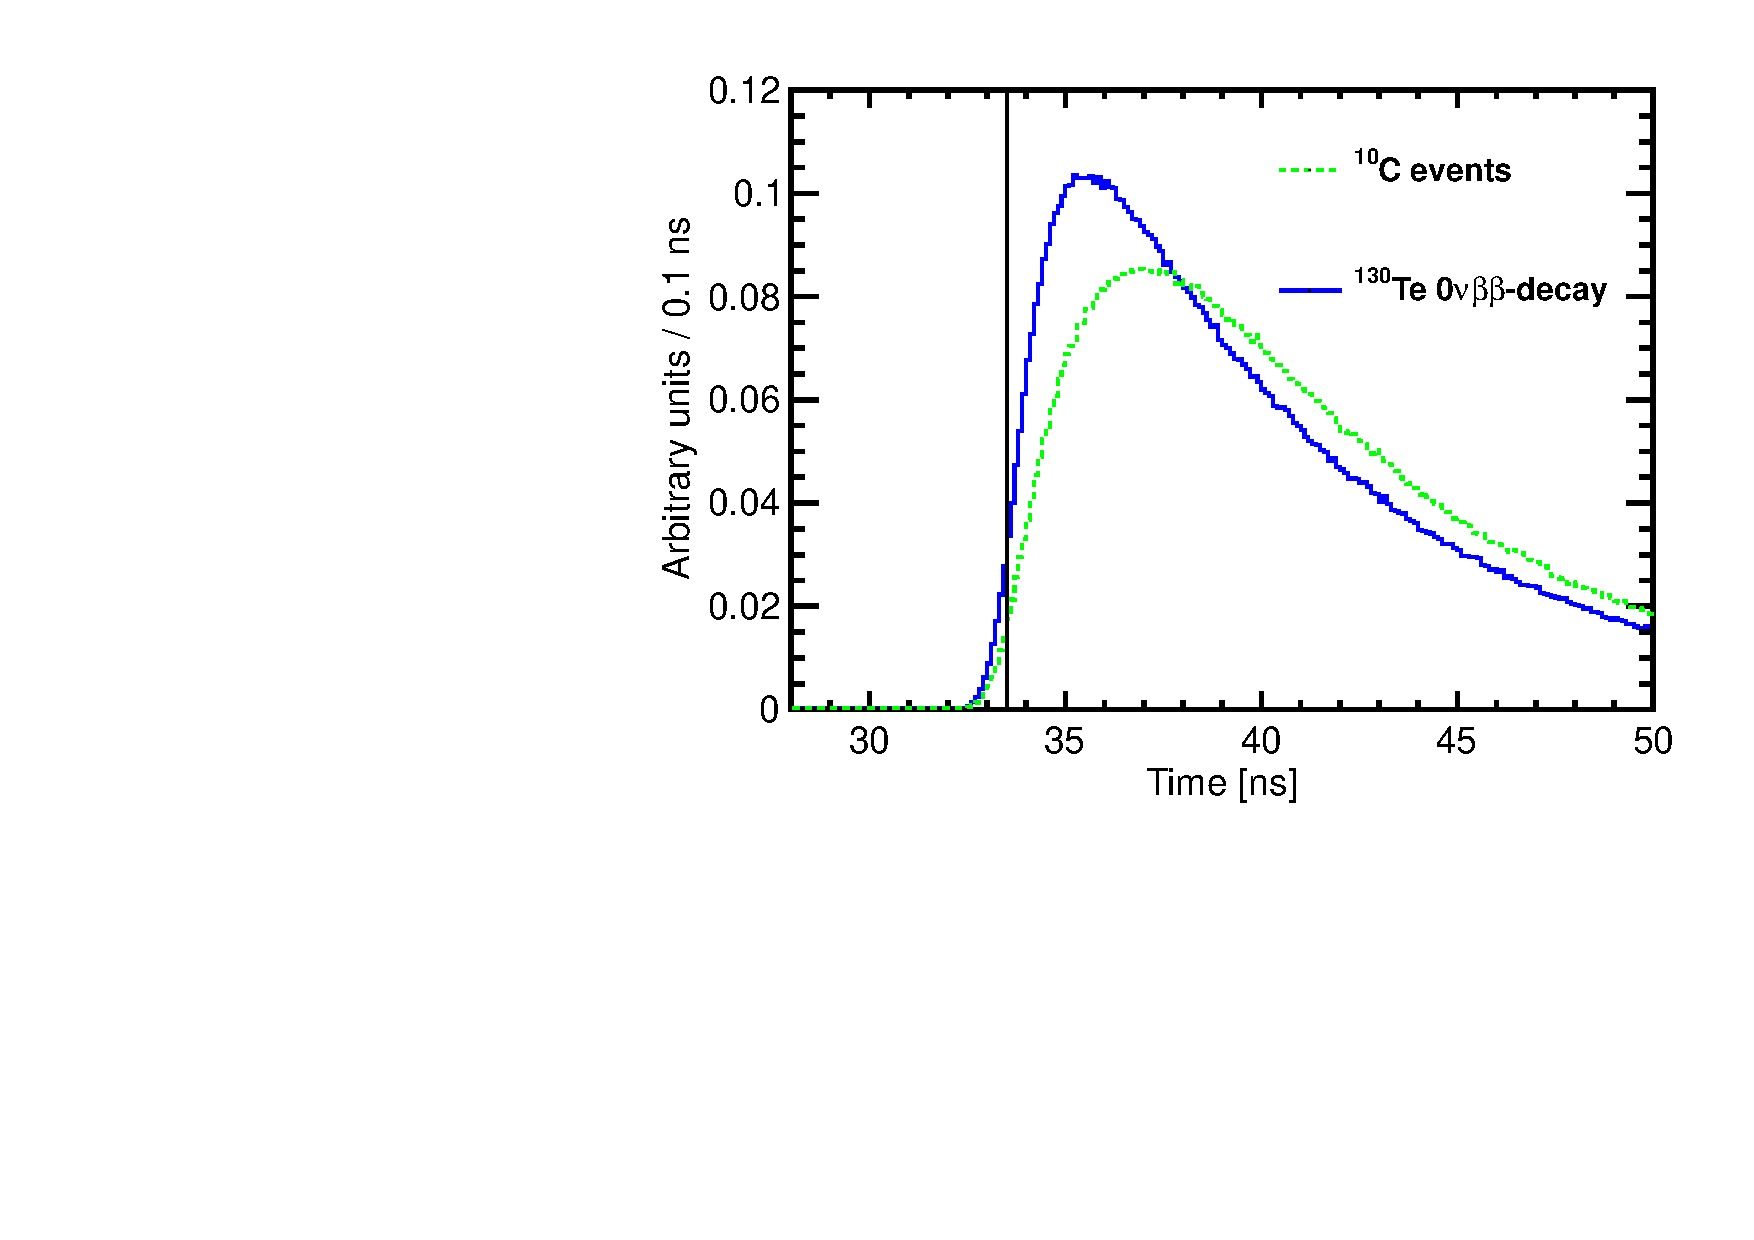
\includegraphics[width=0.45\textwidth]{hT_C10.pdf}
  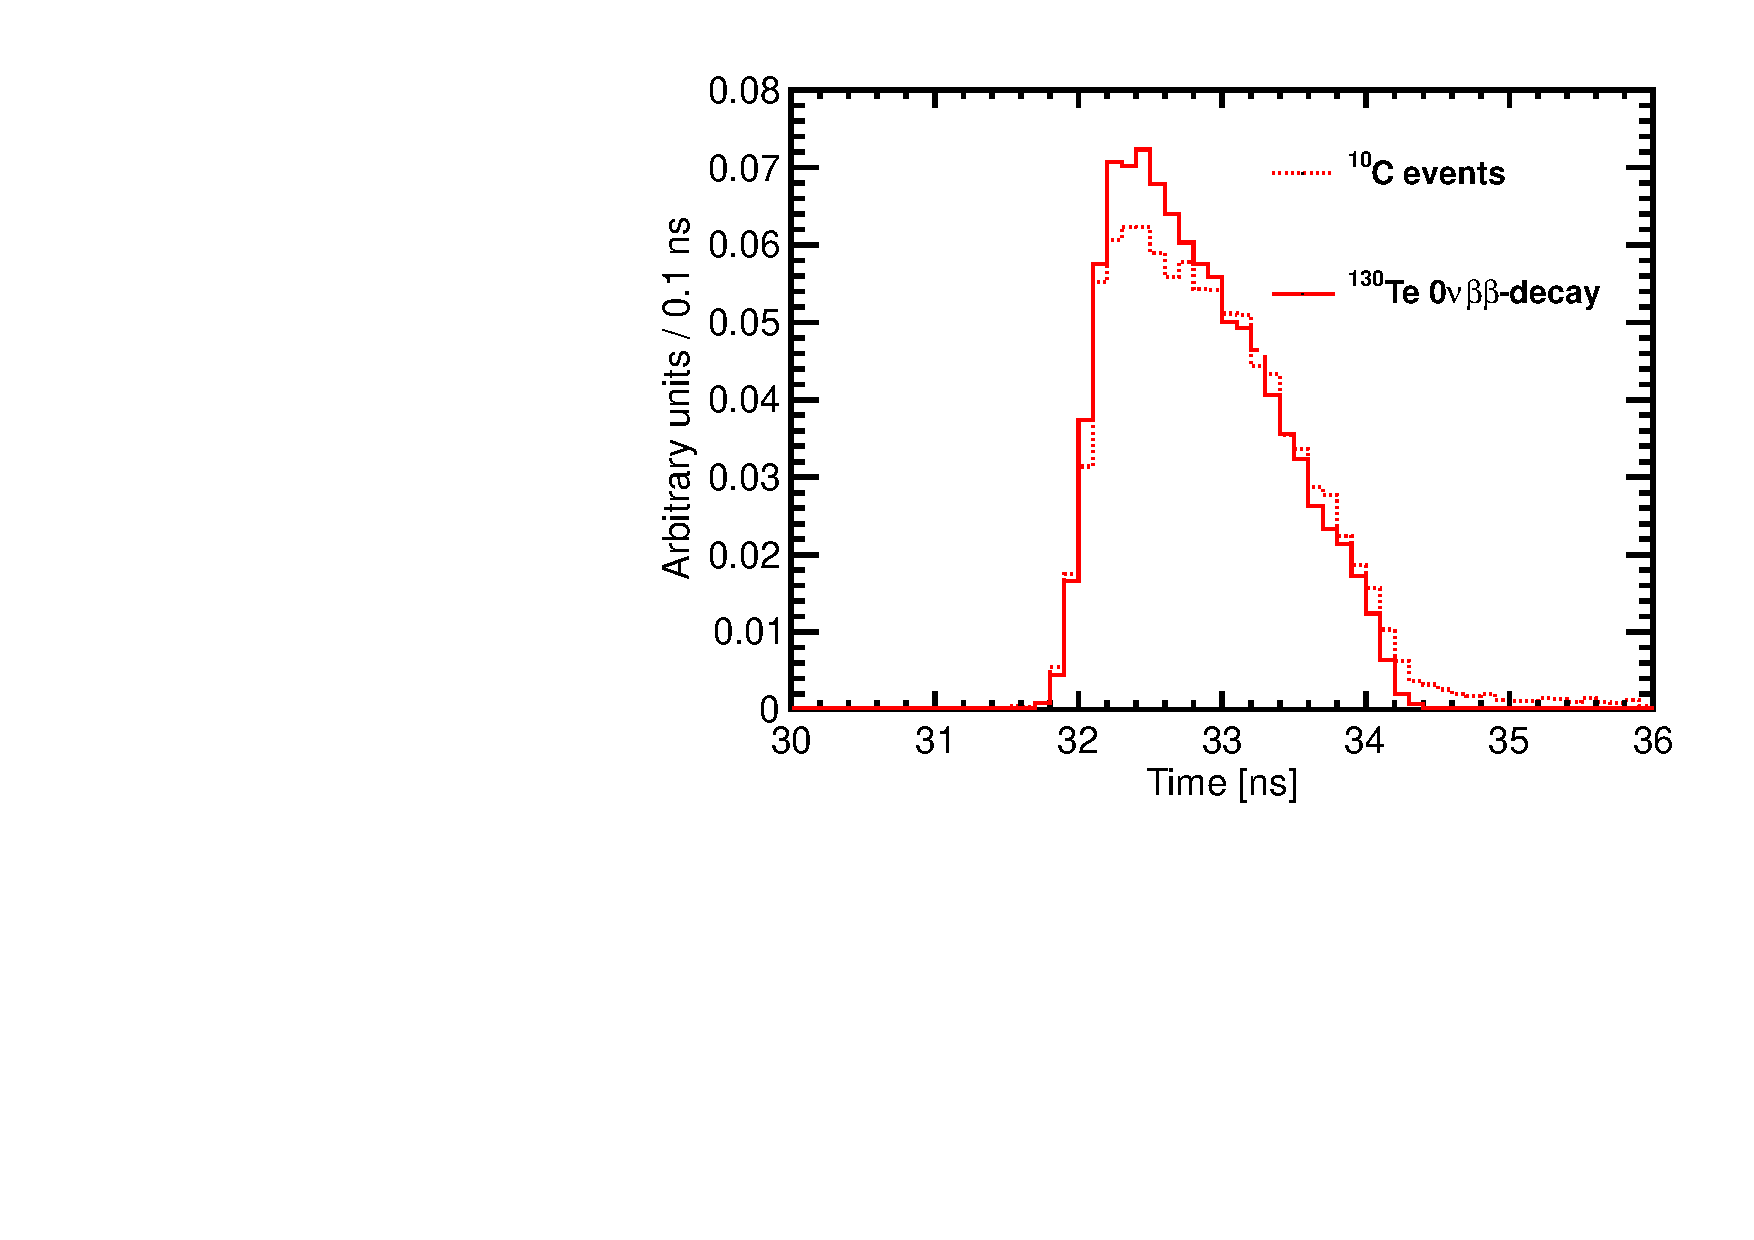
\includegraphics[width=0.45\textwidth]{hTche_C10.pdf}
  \caption{Photo-electron (PE) arrival times after application of the
    photo-detector transit time spread (TTS) of 100~ps for the
    simulation of 1000 0{\nbb} decay events of $^{130}$Te (\emph{solid
      lines}) and $^{10}$C (\emph{dotted lines}) events at the center
    of the detector. All distributions are normalized for shape
    comparison. {\bf Absolute number of PEs per event depends on the
      total energy deposited in the
      detector. Figure~\ref{fig:Edep_C10} shows energy deposited in
      the detector in $^{10}$C events.} \emph{Left:} Scintillation PEs
    arrival time. The black vertical line illustrates a time cut at
    33.5 ns. \emph{Right:} Cherenkov PEs arrival time.}
\label{fig:Arrival_time_C10}
\end{figure}

We note that 98\% of $^{10}$C decays through the excited state of
$^{10}$B(718), which has a half-life time of $\sim$1~ns. Therefore, the
majority of $^{10}$C events have a prompt positron accompanied by a
delayed 0.718~MeV gamma. This delayed gamma affects the PE arrival time
distribution. Figure~\ref{fig:Arrival_time_C10} compares the shape of the
PE arrival time distribution between $^{130}$Te 0{\nbb} decays and
$^{10}$C events. The time profile of the scintillation photons can be used
to separate signal from $^{10}$C events.

\end{comment}

%	!!!!!!!!!!!!!!!!	Commented text ends 	!!!!!!!!!!!!!!!!!!

Comparison of $S_0$ and $S_1$ distributions between 0{\nbb} decay and
$^{10}$C events is shown in Fig.~\ref{fig:S_vs_energy_C10}.

\begin{figure*}[h]
\centering
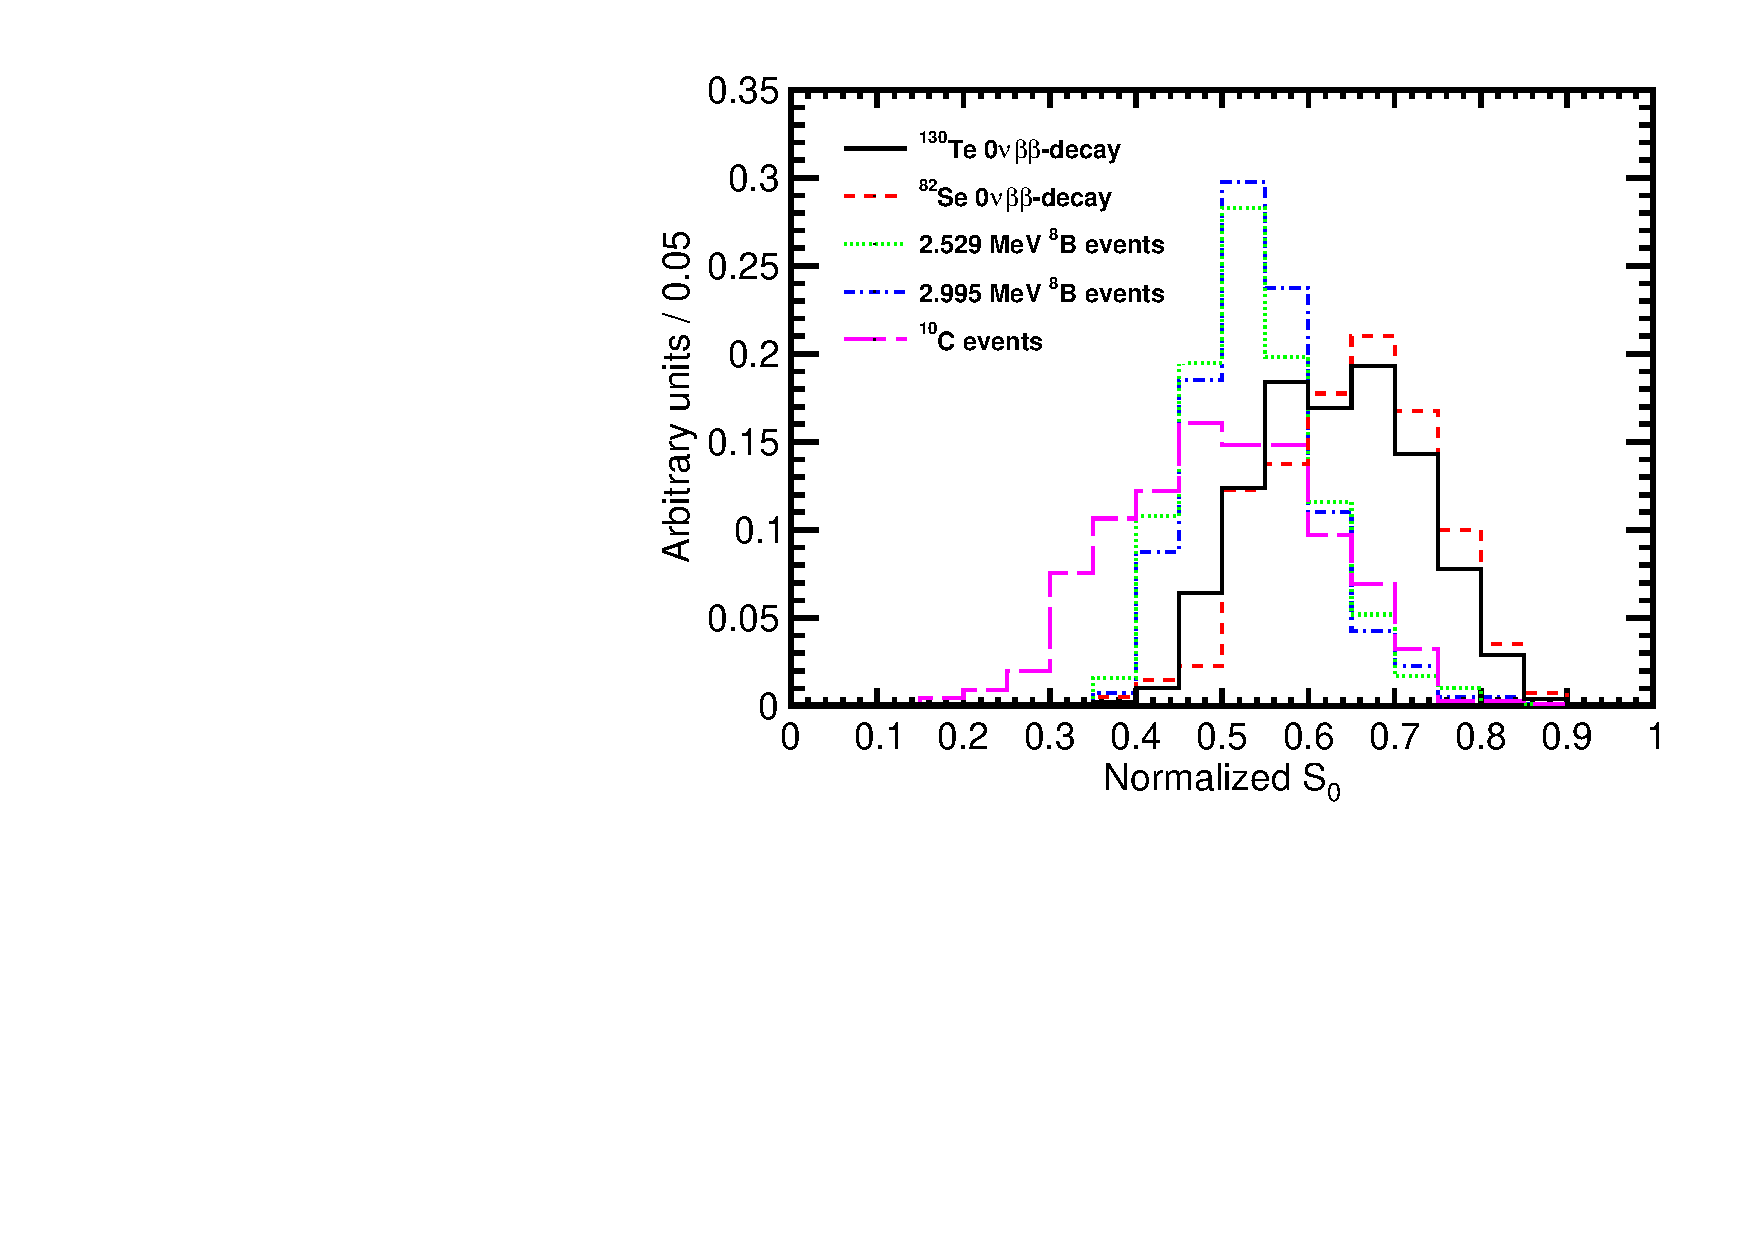
\includegraphics[width=0.49\textwidth]{hS0_C10.pdf}
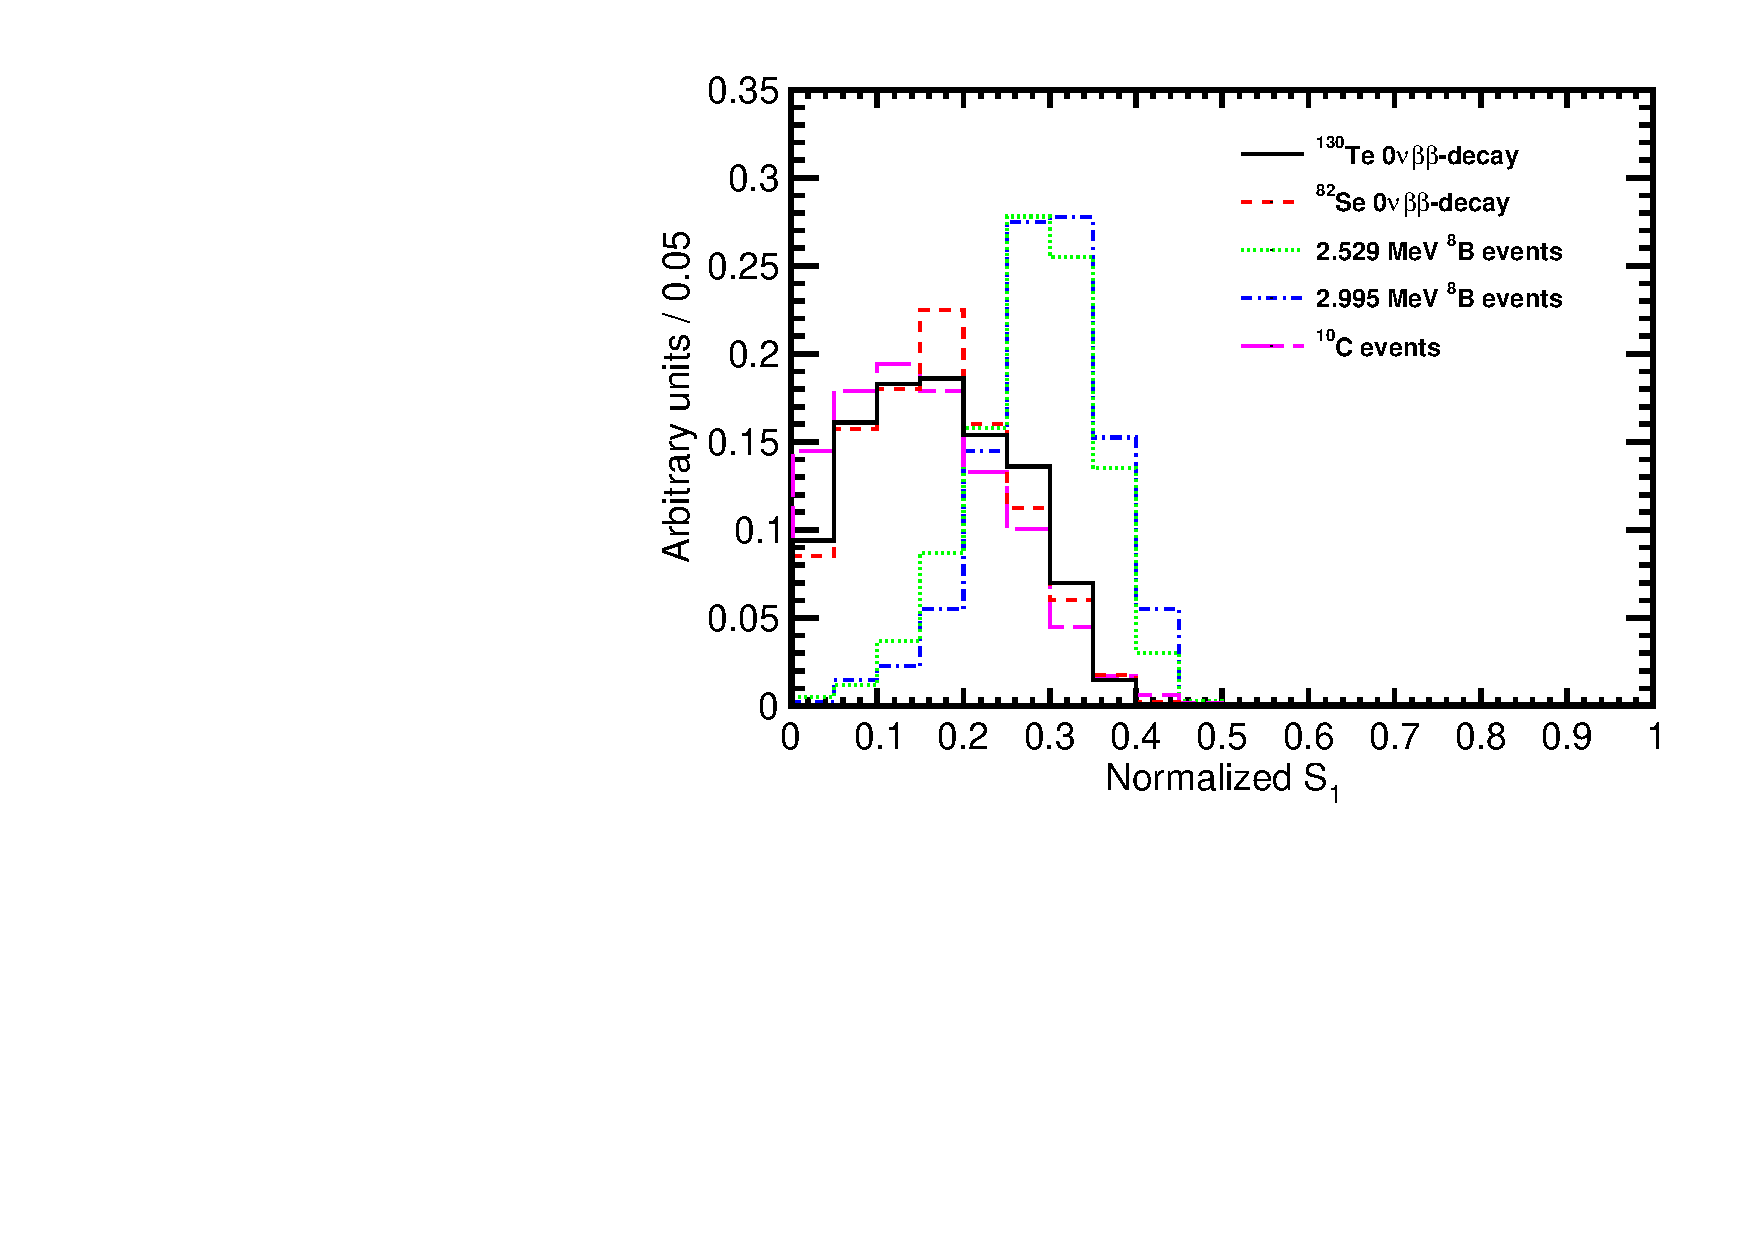
\includegraphics[width=0.49\textwidth]{hS1_C10.pdf}
\caption{$S_0$ (\emph{left}) and $S_1$ (\emph{right}) distributions
  for events with different event topologies. $^{130}$Te, $^{82}$Se 0{\nbb} 
  decays compared with $^{8}$B and $^{10}$C events. The simulation is done 
  for events with the vertex in the center of the detector. $^{8}$B events 
  are implemented as 2.529~MeV or 2.995~MeV electrons with initial direction 
  along $x$-axis. $^{10}$C events are selected in the energy range between 2.1 
  and 2.9~MeV. Perfect vertex reconstruction - true vertex position is used. 
  Time cut of 33.5~ns on the photon arrival time is applied.}
\label{fig:S_vs_energy}
\end{figure*}


\begin{figure}[h]
  \centering
  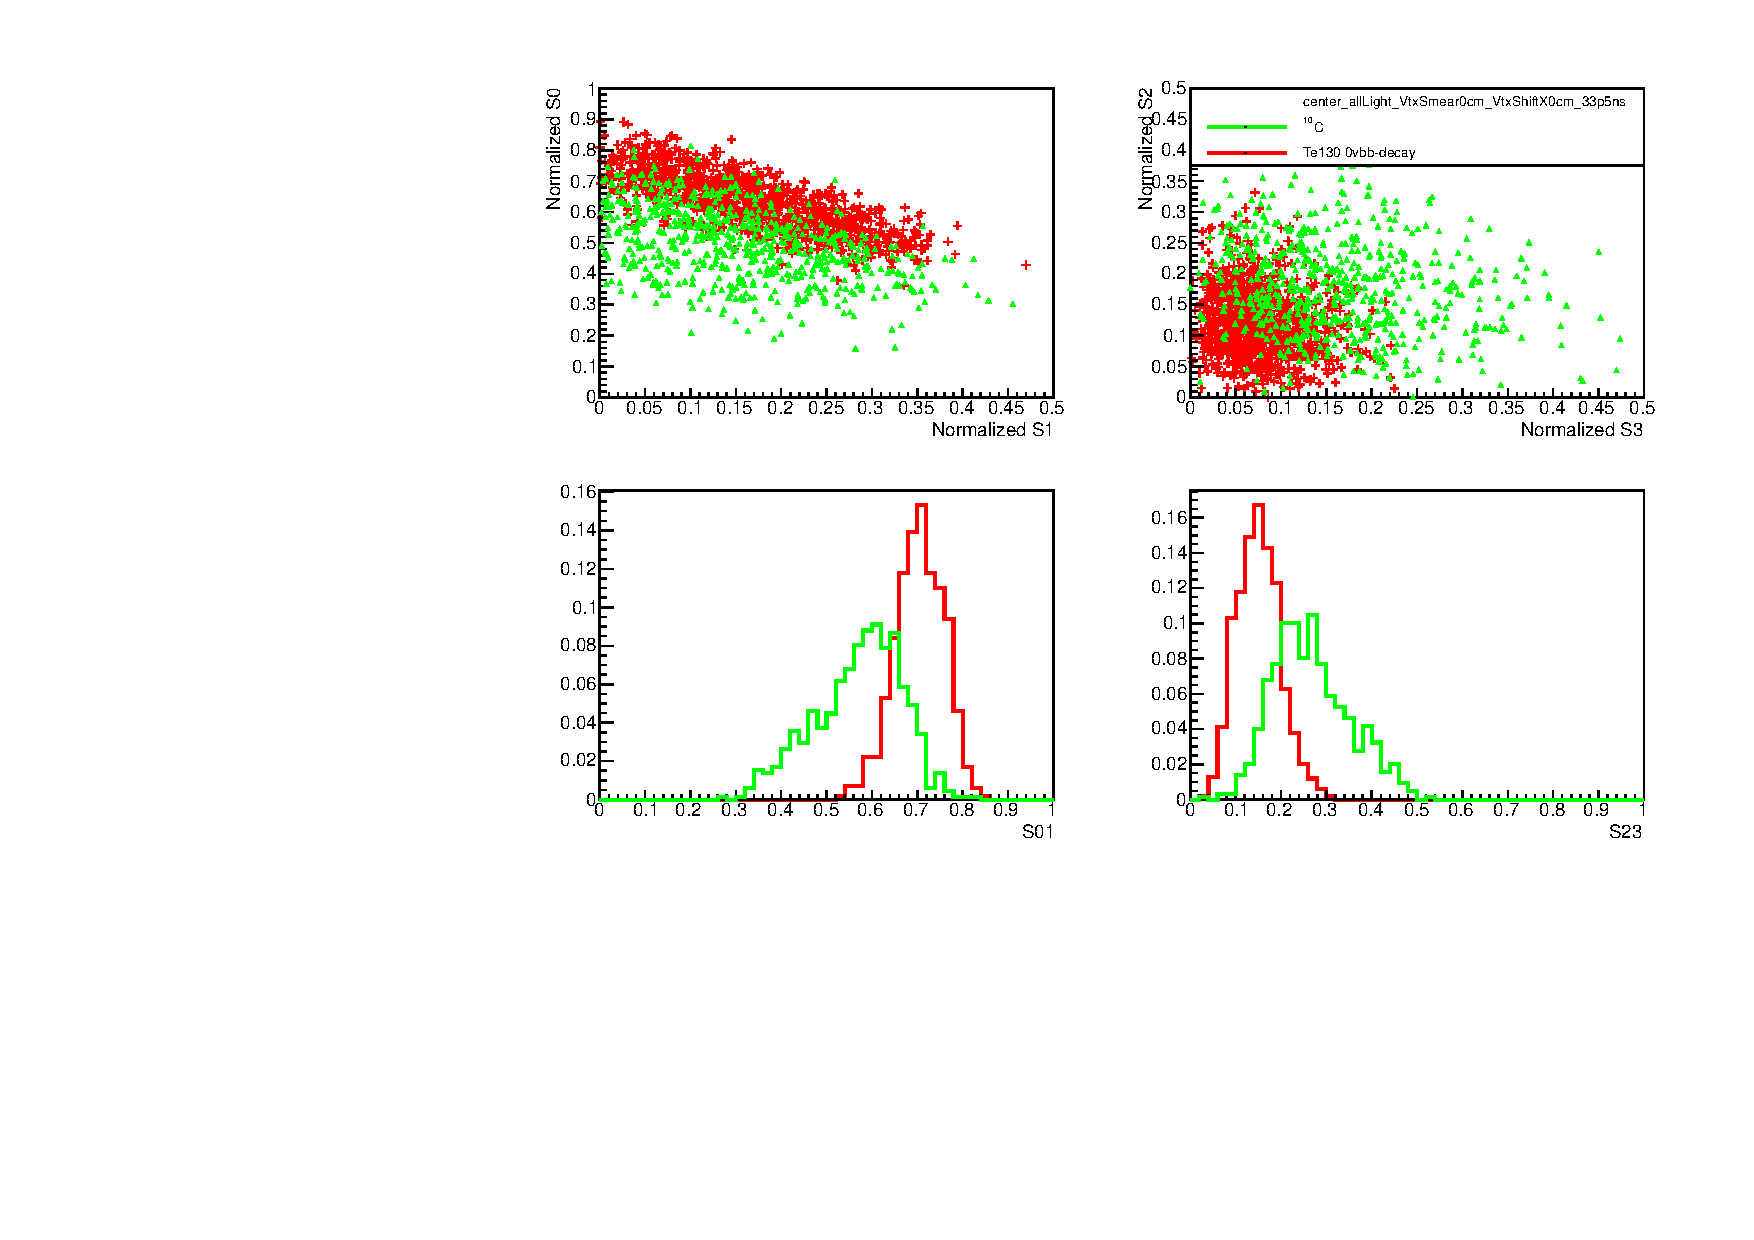
\includegraphics[width=0.95\textwidth]{hSLPlots_C10_allLight_VtxSmear0cm_VtxShiftX0cm_33p5ns_center.pdf}
  \caption{Spherical harmonics comparison between $^{130}$Te 0{\nbb}
    decay signal ($Q=2.529$~MeV) (\emph{red}) and $^{10}$C solar
    neutrinos background (blue) for 1000 simulated events originated
    at the center of the sphere. $^{10}$C with energy deposition
    between 2.1~MeV and 2.9~MeV are considered. Perfect vertex
    reconstruction - true vertex position is used. Time cut of 33.5~ns
    on the photon arrival time is applied. \emph{Top left:} S$_0$
    versus S$_1$ scatter plot. \emph{Top right:} S$_2$ versus S$_3$
    scatter plot. \emph{Bottom left:} Distribution of the
    S$^{C10}_{01}$ variable calculated for signal (\emph{red}) and
    background (\emph{green}). \emph{Bottom right:} Distribution of
    the S$^{C10}_{23}$ variable calculated for signal (\emph{red}) and
    background (\emph{green}).}
  \label{fig:SL_C10_33p5ns_center}
\end{figure}


Comparison of spherical harmonics is shown in
Fig.~\ref{fig:SL_C10_33p5ns_center}. $^{10}$C events are generated at
the center of the detector. True vertex position is used to apply a
33.5~ns time cut to select photons for the spherical harmonics
analysis. The separation is seen in S0 vs S1 and S2 vs S3 scatter
plots. We project both scatter plots to a line that gives maximum
separation (two bottom panels in Fig.~\ref{fig:SL_C10_33p5ns_center}).  
There is enough separation between the distributions to suggest that this analysis can be used to distinguish between 0{\nbb} and $^{10}$C events.

%\section{0{\nbb} decay vs backgrounds from Th and U series}



\end{document}

